\documentclass[]{book}
\usepackage{lmodern}
\usepackage{amssymb,amsmath}
\usepackage{ifxetex,ifluatex}
\usepackage{fixltx2e} % provides \textsubscript
\ifnum 0\ifxetex 1\fi\ifluatex 1\fi=0 % if pdftex
  \usepackage[T1]{fontenc}
  \usepackage[utf8]{inputenc}
\else % if luatex or xelatex
  \ifxetex
    \usepackage{mathspec}
  \else
    \usepackage{fontspec}
  \fi
  \defaultfontfeatures{Ligatures=TeX,Scale=MatchLowercase}
\fi
% use upquote if available, for straight quotes in verbatim environments
\IfFileExists{upquote.sty}{\usepackage{upquote}}{}
% use microtype if available
\IfFileExists{microtype.sty}{%
\usepackage{microtype}
\UseMicrotypeSet[protrusion]{basicmath} % disable protrusion for tt fonts
}{}
\usepackage[margin=1in]{geometry}
\usepackage{hyperref}
\hypersetup{unicode=true,
            pdftitle={OpenIntro Statistics: Labs for R},
            pdfauthor={Andrew Bray; Mine Çetinkaya-Rundel; Arend Kuyper},
            pdfborder={0 0 0},
            breaklinks=true}
\urlstyle{same}  % don't use monospace font for urls
\usepackage{natbib}
\bibliographystyle{apalike}
\usepackage{color}
\usepackage{fancyvrb}
\newcommand{\VerbBar}{|}
\newcommand{\VERB}{\Verb[commandchars=\\\{\}]}
\DefineVerbatimEnvironment{Highlighting}{Verbatim}{commandchars=\\\{\}}
% Add ',fontsize=\small' for more characters per line
\usepackage{framed}
\definecolor{shadecolor}{RGB}{248,248,248}
\newenvironment{Shaded}{\begin{snugshade}}{\end{snugshade}}
\newcommand{\KeywordTok}[1]{\textcolor[rgb]{0.13,0.29,0.53}{\textbf{{#1}}}}
\newcommand{\DataTypeTok}[1]{\textcolor[rgb]{0.13,0.29,0.53}{{#1}}}
\newcommand{\DecValTok}[1]{\textcolor[rgb]{0.00,0.00,0.81}{{#1}}}
\newcommand{\BaseNTok}[1]{\textcolor[rgb]{0.00,0.00,0.81}{{#1}}}
\newcommand{\FloatTok}[1]{\textcolor[rgb]{0.00,0.00,0.81}{{#1}}}
\newcommand{\ConstantTok}[1]{\textcolor[rgb]{0.00,0.00,0.00}{{#1}}}
\newcommand{\CharTok}[1]{\textcolor[rgb]{0.31,0.60,0.02}{{#1}}}
\newcommand{\SpecialCharTok}[1]{\textcolor[rgb]{0.00,0.00,0.00}{{#1}}}
\newcommand{\StringTok}[1]{\textcolor[rgb]{0.31,0.60,0.02}{{#1}}}
\newcommand{\VerbatimStringTok}[1]{\textcolor[rgb]{0.31,0.60,0.02}{{#1}}}
\newcommand{\SpecialStringTok}[1]{\textcolor[rgb]{0.31,0.60,0.02}{{#1}}}
\newcommand{\ImportTok}[1]{{#1}}
\newcommand{\CommentTok}[1]{\textcolor[rgb]{0.56,0.35,0.01}{\textit{{#1}}}}
\newcommand{\DocumentationTok}[1]{\textcolor[rgb]{0.56,0.35,0.01}{\textbf{\textit{{#1}}}}}
\newcommand{\AnnotationTok}[1]{\textcolor[rgb]{0.56,0.35,0.01}{\textbf{\textit{{#1}}}}}
\newcommand{\CommentVarTok}[1]{\textcolor[rgb]{0.56,0.35,0.01}{\textbf{\textit{{#1}}}}}
\newcommand{\OtherTok}[1]{\textcolor[rgb]{0.56,0.35,0.01}{{#1}}}
\newcommand{\FunctionTok}[1]{\textcolor[rgb]{0.00,0.00,0.00}{{#1}}}
\newcommand{\VariableTok}[1]{\textcolor[rgb]{0.00,0.00,0.00}{{#1}}}
\newcommand{\ControlFlowTok}[1]{\textcolor[rgb]{0.13,0.29,0.53}{\textbf{{#1}}}}
\newcommand{\OperatorTok}[1]{\textcolor[rgb]{0.81,0.36,0.00}{\textbf{{#1}}}}
\newcommand{\BuiltInTok}[1]{{#1}}
\newcommand{\ExtensionTok}[1]{{#1}}
\newcommand{\PreprocessorTok}[1]{\textcolor[rgb]{0.56,0.35,0.01}{\textit{{#1}}}}
\newcommand{\AttributeTok}[1]{\textcolor[rgb]{0.77,0.63,0.00}{{#1}}}
\newcommand{\RegionMarkerTok}[1]{{#1}}
\newcommand{\InformationTok}[1]{\textcolor[rgb]{0.56,0.35,0.01}{\textbf{\textit{{#1}}}}}
\newcommand{\WarningTok}[1]{\textcolor[rgb]{0.56,0.35,0.01}{\textbf{\textit{{#1}}}}}
\newcommand{\AlertTok}[1]{\textcolor[rgb]{0.94,0.16,0.16}{{#1}}}
\newcommand{\ErrorTok}[1]{\textcolor[rgb]{0.64,0.00,0.00}{\textbf{{#1}}}}
\newcommand{\NormalTok}[1]{{#1}}
\usepackage{longtable,booktabs}
\usepackage{graphicx,grffile}
\makeatletter
\def\maxwidth{\ifdim\Gin@nat@width>\linewidth\linewidth\else\Gin@nat@width\fi}
\def\maxheight{\ifdim\Gin@nat@height>\textheight\textheight\else\Gin@nat@height\fi}
\makeatother
% Scale images if necessary, so that they will not overflow the page
% margins by default, and it is still possible to overwrite the defaults
% using explicit options in \includegraphics[width, height, ...]{}
\setkeys{Gin}{width=\maxwidth,height=\maxheight,keepaspectratio}
\IfFileExists{parskip.sty}{%
\usepackage{parskip}
}{% else
\setlength{\parindent}{0pt}
\setlength{\parskip}{6pt plus 2pt minus 1pt}
}
\setlength{\emergencystretch}{3em}  % prevent overfull lines
\providecommand{\tightlist}{%
  \setlength{\itemsep}{0pt}\setlength{\parskip}{0pt}}
\setcounter{secnumdepth}{5}
% Redefines (sub)paragraphs to behave more like sections
\ifx\paragraph\undefined\else
\let\oldparagraph\paragraph
\renewcommand{\paragraph}[1]{\oldparagraph{#1}\mbox{}}
\fi
\ifx\subparagraph\undefined\else
\let\oldsubparagraph\subparagraph
\renewcommand{\subparagraph}[1]{\oldsubparagraph{#1}\mbox{}}
\fi

%%% Use protect on footnotes to avoid problems with footnotes in titles
\let\rmarkdownfootnote\footnote%
\def\footnote{\protect\rmarkdownfootnote}

%%% Change title format to be more compact
\usepackage{titling}

% Create subtitle command for use in maketitle
\newcommand{\subtitle}[1]{
  \posttitle{
    \begin{center}\large#1\end{center}
    }
}

\setlength{\droptitle}{-2em}
  \title{OpenIntro Statistics: Labs for R}
  \pretitle{\vspace{\droptitle}\centering\huge}
  \posttitle{\par}
  \author{Andrew Bray \\ Mine Çetinkaya-Rundel \\ Arend Kuyper}
  \preauthor{\centering\large\emph}
  \postauthor{\par}
  \predate{\centering\large\emph}
  \postdate{\par}
  \date{2018}

\usepackage{booktabs}

\usepackage{amsthm}
\newtheorem{theorem}{Theorem}[chapter]
\newtheorem{lemma}{Lemma}[chapter]
\theoremstyle{definition}
\newtheorem{definition}{Definition}[chapter]
\newtheorem{corollary}{Corollary}[chapter]
\newtheorem{proposition}{Proposition}[chapter]
\theoremstyle{definition}
\newtheorem{example}{Example}[chapter]
\theoremstyle{definition}
\newtheorem{exercise}{Exercise}[chapter]
\theoremstyle{remark}
\newtheorem*{remark}{Remark}
\newtheorem*{solution}{Solution}
\begin{document}
\maketitle

{
\setcounter{tocdepth}{1}
\tableofcontents
}
\chapter*{Preface}\label{preface}
\addcontentsline{toc}{chapter}{Preface}

These lab exercises supplement the third edition of
\href{https://www.openintro.org/stat/index.php}{OpenIntro Statistics}
textbook. Each lab steps through the process of using the R programming
language for collecting, analyzing, and using statistical data to make
inferences and conclusions about real world phenomena.

This version of the labs have been modified by
\href{https://www.statistics.northwestern.edu/people/faculty/arend-m-kuyper.html}{Arend
Kuyper} to include new datasets and examples for introductory statistics
courses at Northwestern University. Visit
\href{https://www.openintro.org/stat/labs.php}{Labs for R} at OpenIntro
for the original materials. The chapters in this book were adapted from
labs originally written by Mark Hansen and adapted for OpenIntro by
Andrew Bray and Mine Çetinkaya-Rundel.

\section{Using these labs}\label{using-these-labs}

All of the labs on this website are made available under a
\href{https://creativecommons.org/licenses/by-sa/3.0/}{Creative Commons
Attribution-ShareAlike license}. You are free to copy, redistribute, and
modify the material in any format so long as you provide attribution.
Any derivative versions of the content must be distributed under the
same license.

\begin{figure}[htbp]
\centering

\includegraphics{./assets/images/by-sa.png}
\caption{Creative Commons Attribution ShareAlike}
\end{figure}

\chapter{Working Efficiently with
RStudio}\label{working-efficiently-with-rstudio}

\section{Why RStudio?}\label{why-rstudio}

RStudio is an extremely powerful tool that is intended to optimize how
we interact with the statistical software known as
\href{https://www.r-project.org/about.html}{R}. We could use R's basic
interface, but \href{https://www.rstudio.com/}{RStudio} is designed to
streamline and organize statistical and analytic work with R. Like any
tool we must learn how to use it properly, which is the focus of this
lab.

While it might seem clunky or cumbersome at first, it is important to
discipline yourself and adhere to sound workflow practices. Doing this
from the very beginning will payoff immensely in later labs and beyond
--- whether or not you intend to work with RStudio in the future.
Exercising and expanding your mind to preform analytic coding will make
you a better critical thinker and problem solver.

\begin{center}\rule{0.5\linewidth}{\linethickness}\end{center}

\section{Setting Up an R Project}\label{setting-up-an-r-project}

It is important to recognize that quality analytic work requires that
your work be easy to follow, replicate, and reference by others or by
the future you. Therefore it is imperative that you strive to be as
organized as possible. RStudio helps you organize all your work on a
given data analysis/project through the creation of R projects.

There are several ways one could go about creating an R project, but we
would suggest following the steps outlined below. These steps outline
how to get setup for the first lab, but should, with obvious
alterations, be followed for each lab.

\textbf{Step 1}

Create a folder somewhere on your computer, say on your desktop, and
give it a descriptive name (e.g.~STAT 202). This folder is where you
will keep all of your work for each lab. You could save all your
electronic notes here too.

\textbf{Step 2}

Next you will want to create a subfolder for an individual task or
sub-project (e.g. \textbf{Lab 01}). The graphic below displays an
example folder structure.

\begin{figure}[htbp]
\centering
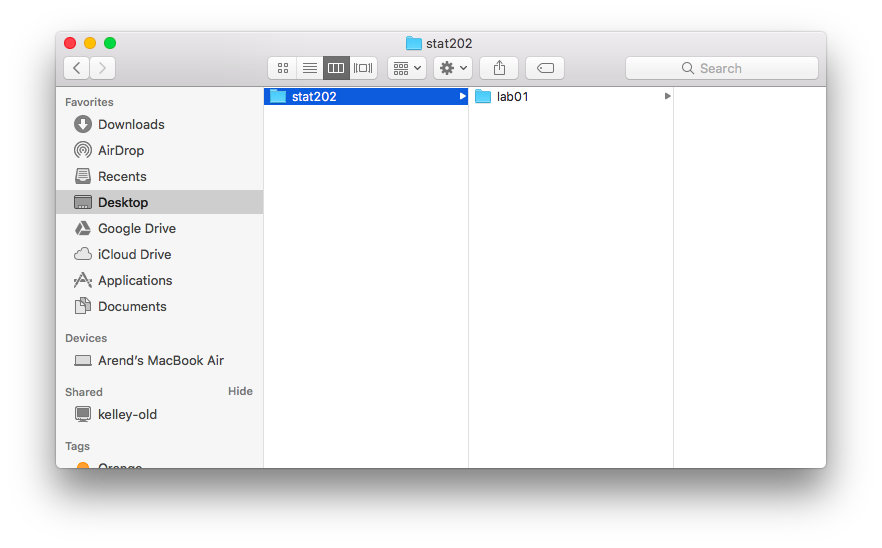
\includegraphics{./assets/images/01-01.png}
\caption{}
\end{figure}

\textbf{Step 3}

Open RStudio.

\textbf{Step 4}

\begin{enumerate}
\def\labelenumi{\arabic{enumi}.}
\setcounter{enumi}{3}
\tightlist
\item
  Create a project by navigating to the upper right-hand corner of the
  program and clicking \textbf{Project (None) » New Project}.
\end{enumerate}

\begin{figure}[htbp]
\centering
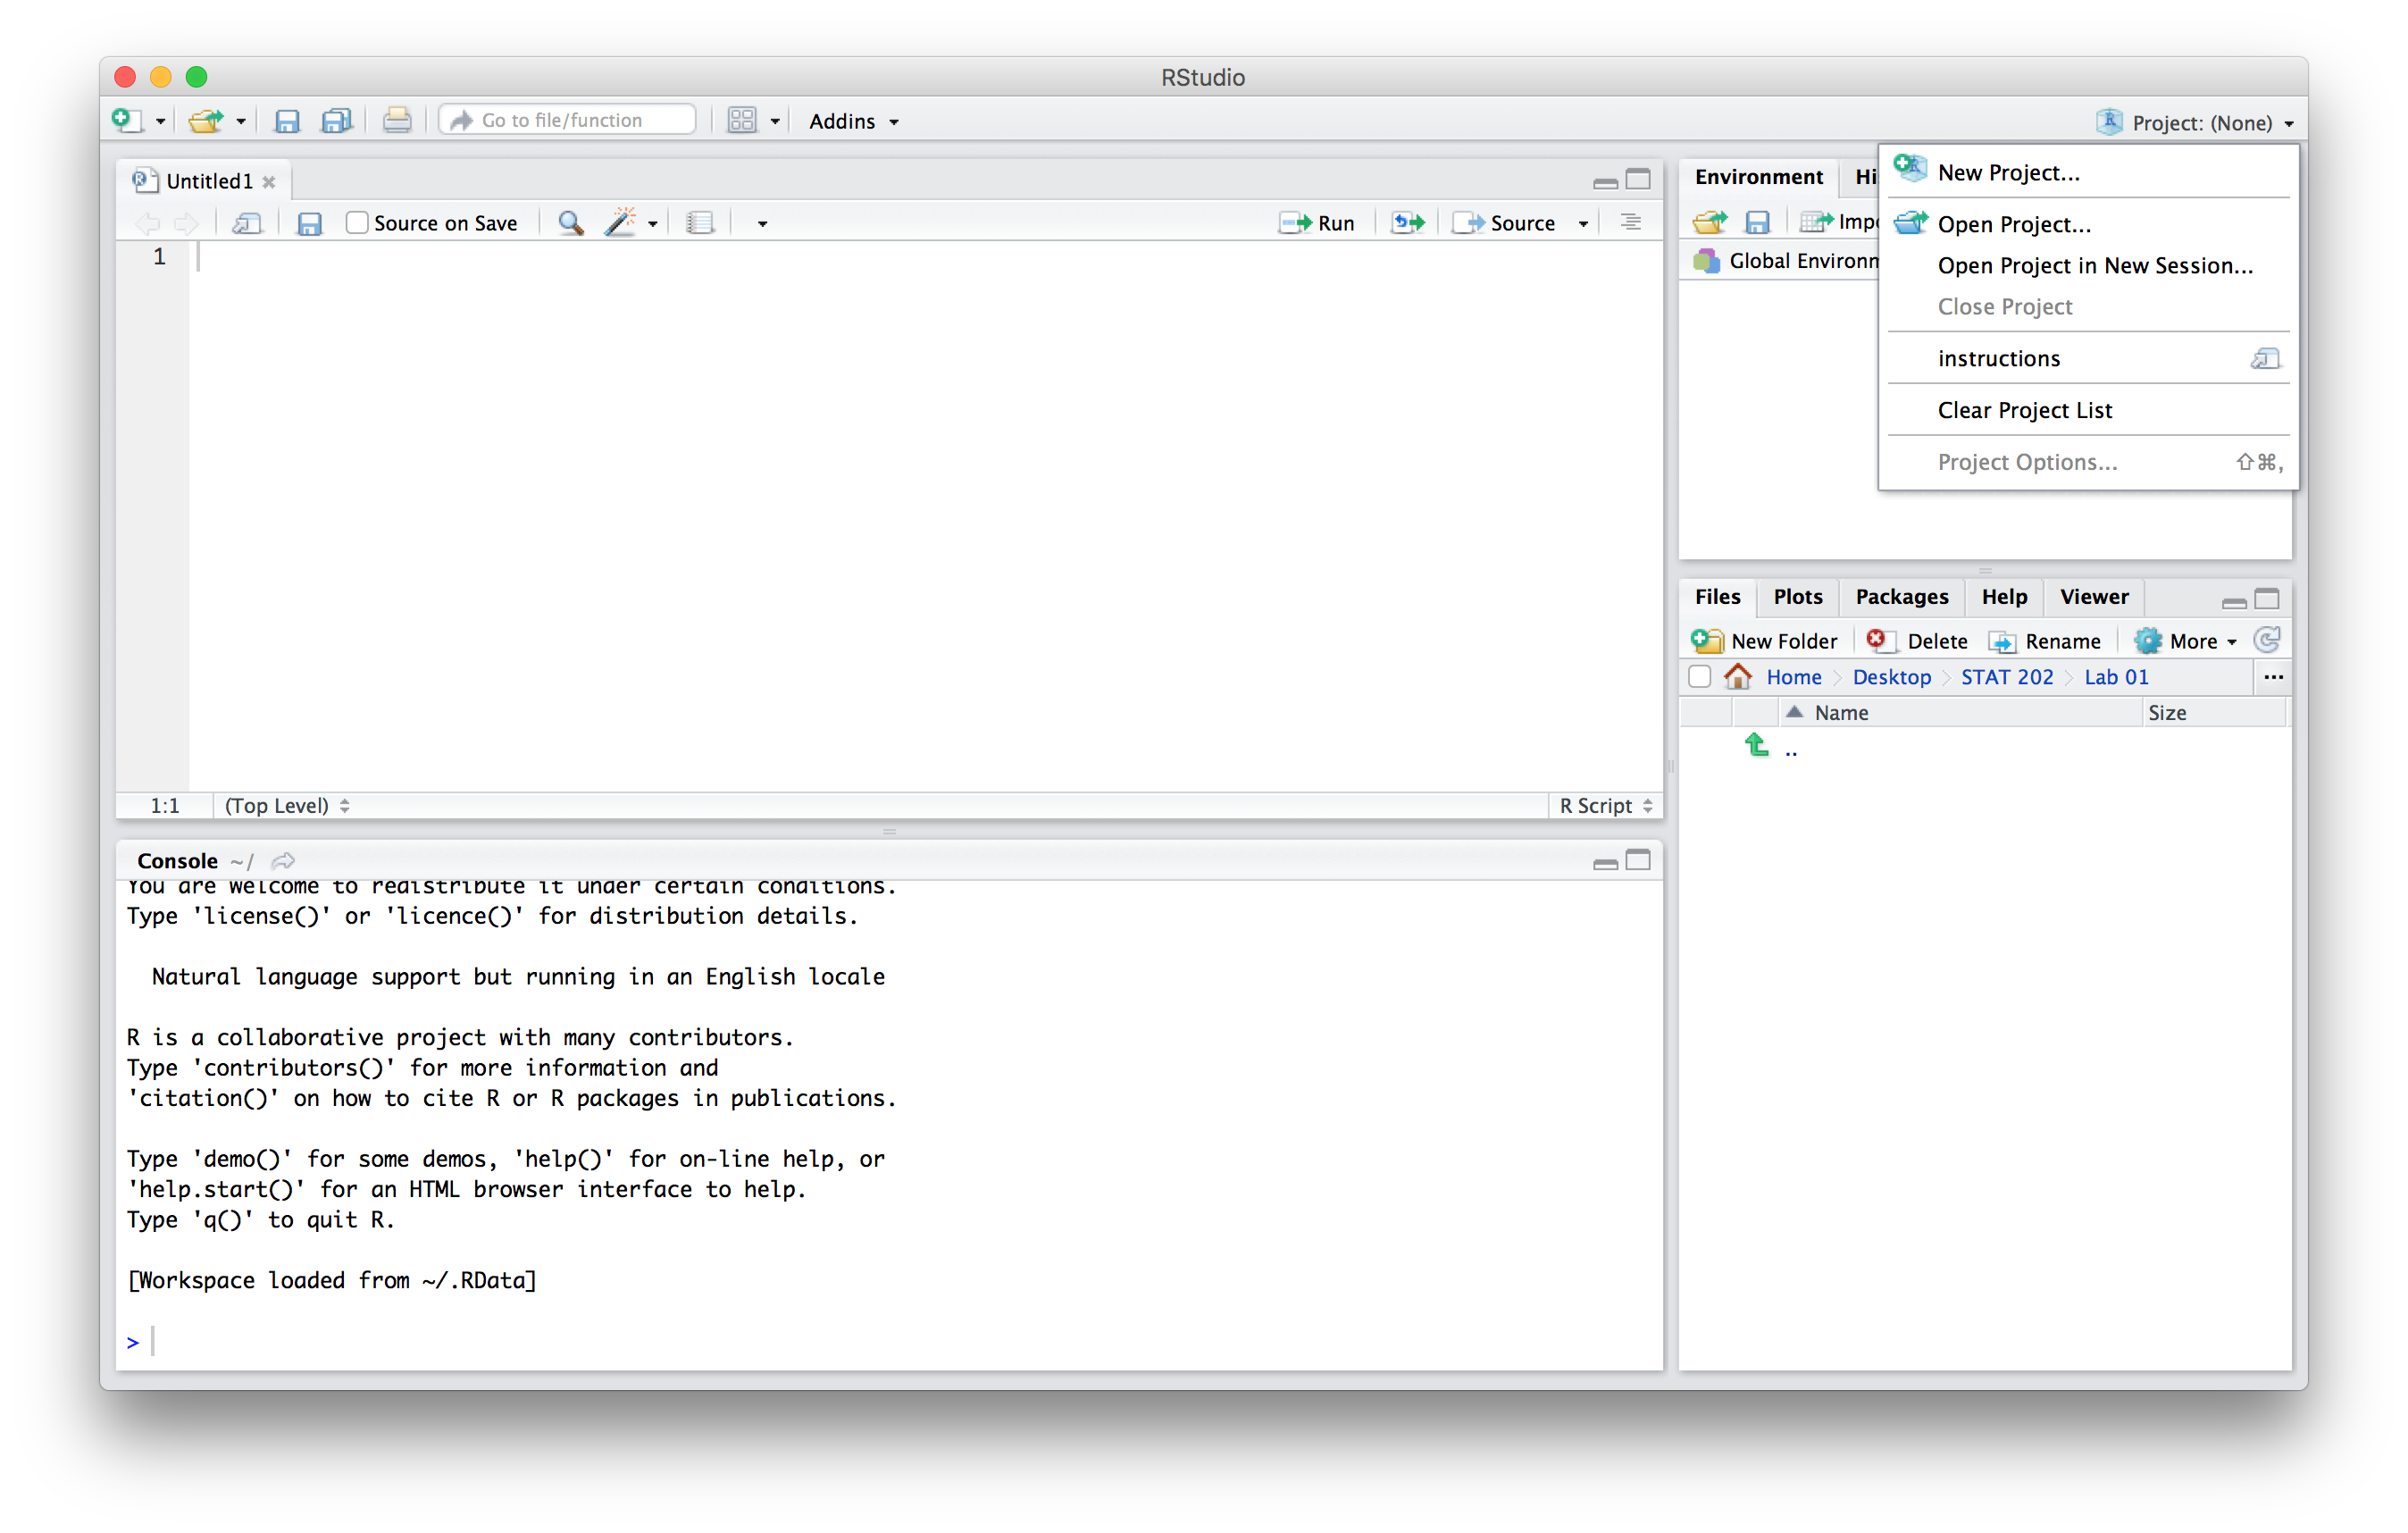
\includegraphics{./assets/images/01-02.png}
\caption{}
\end{figure}

\textbf{Step 5}

Select \textbf{Existing Directory}. Recall that in step 1, you created a
file location for lab 1 --- our data analysis project.

\begin{figure}[htbp]
\centering
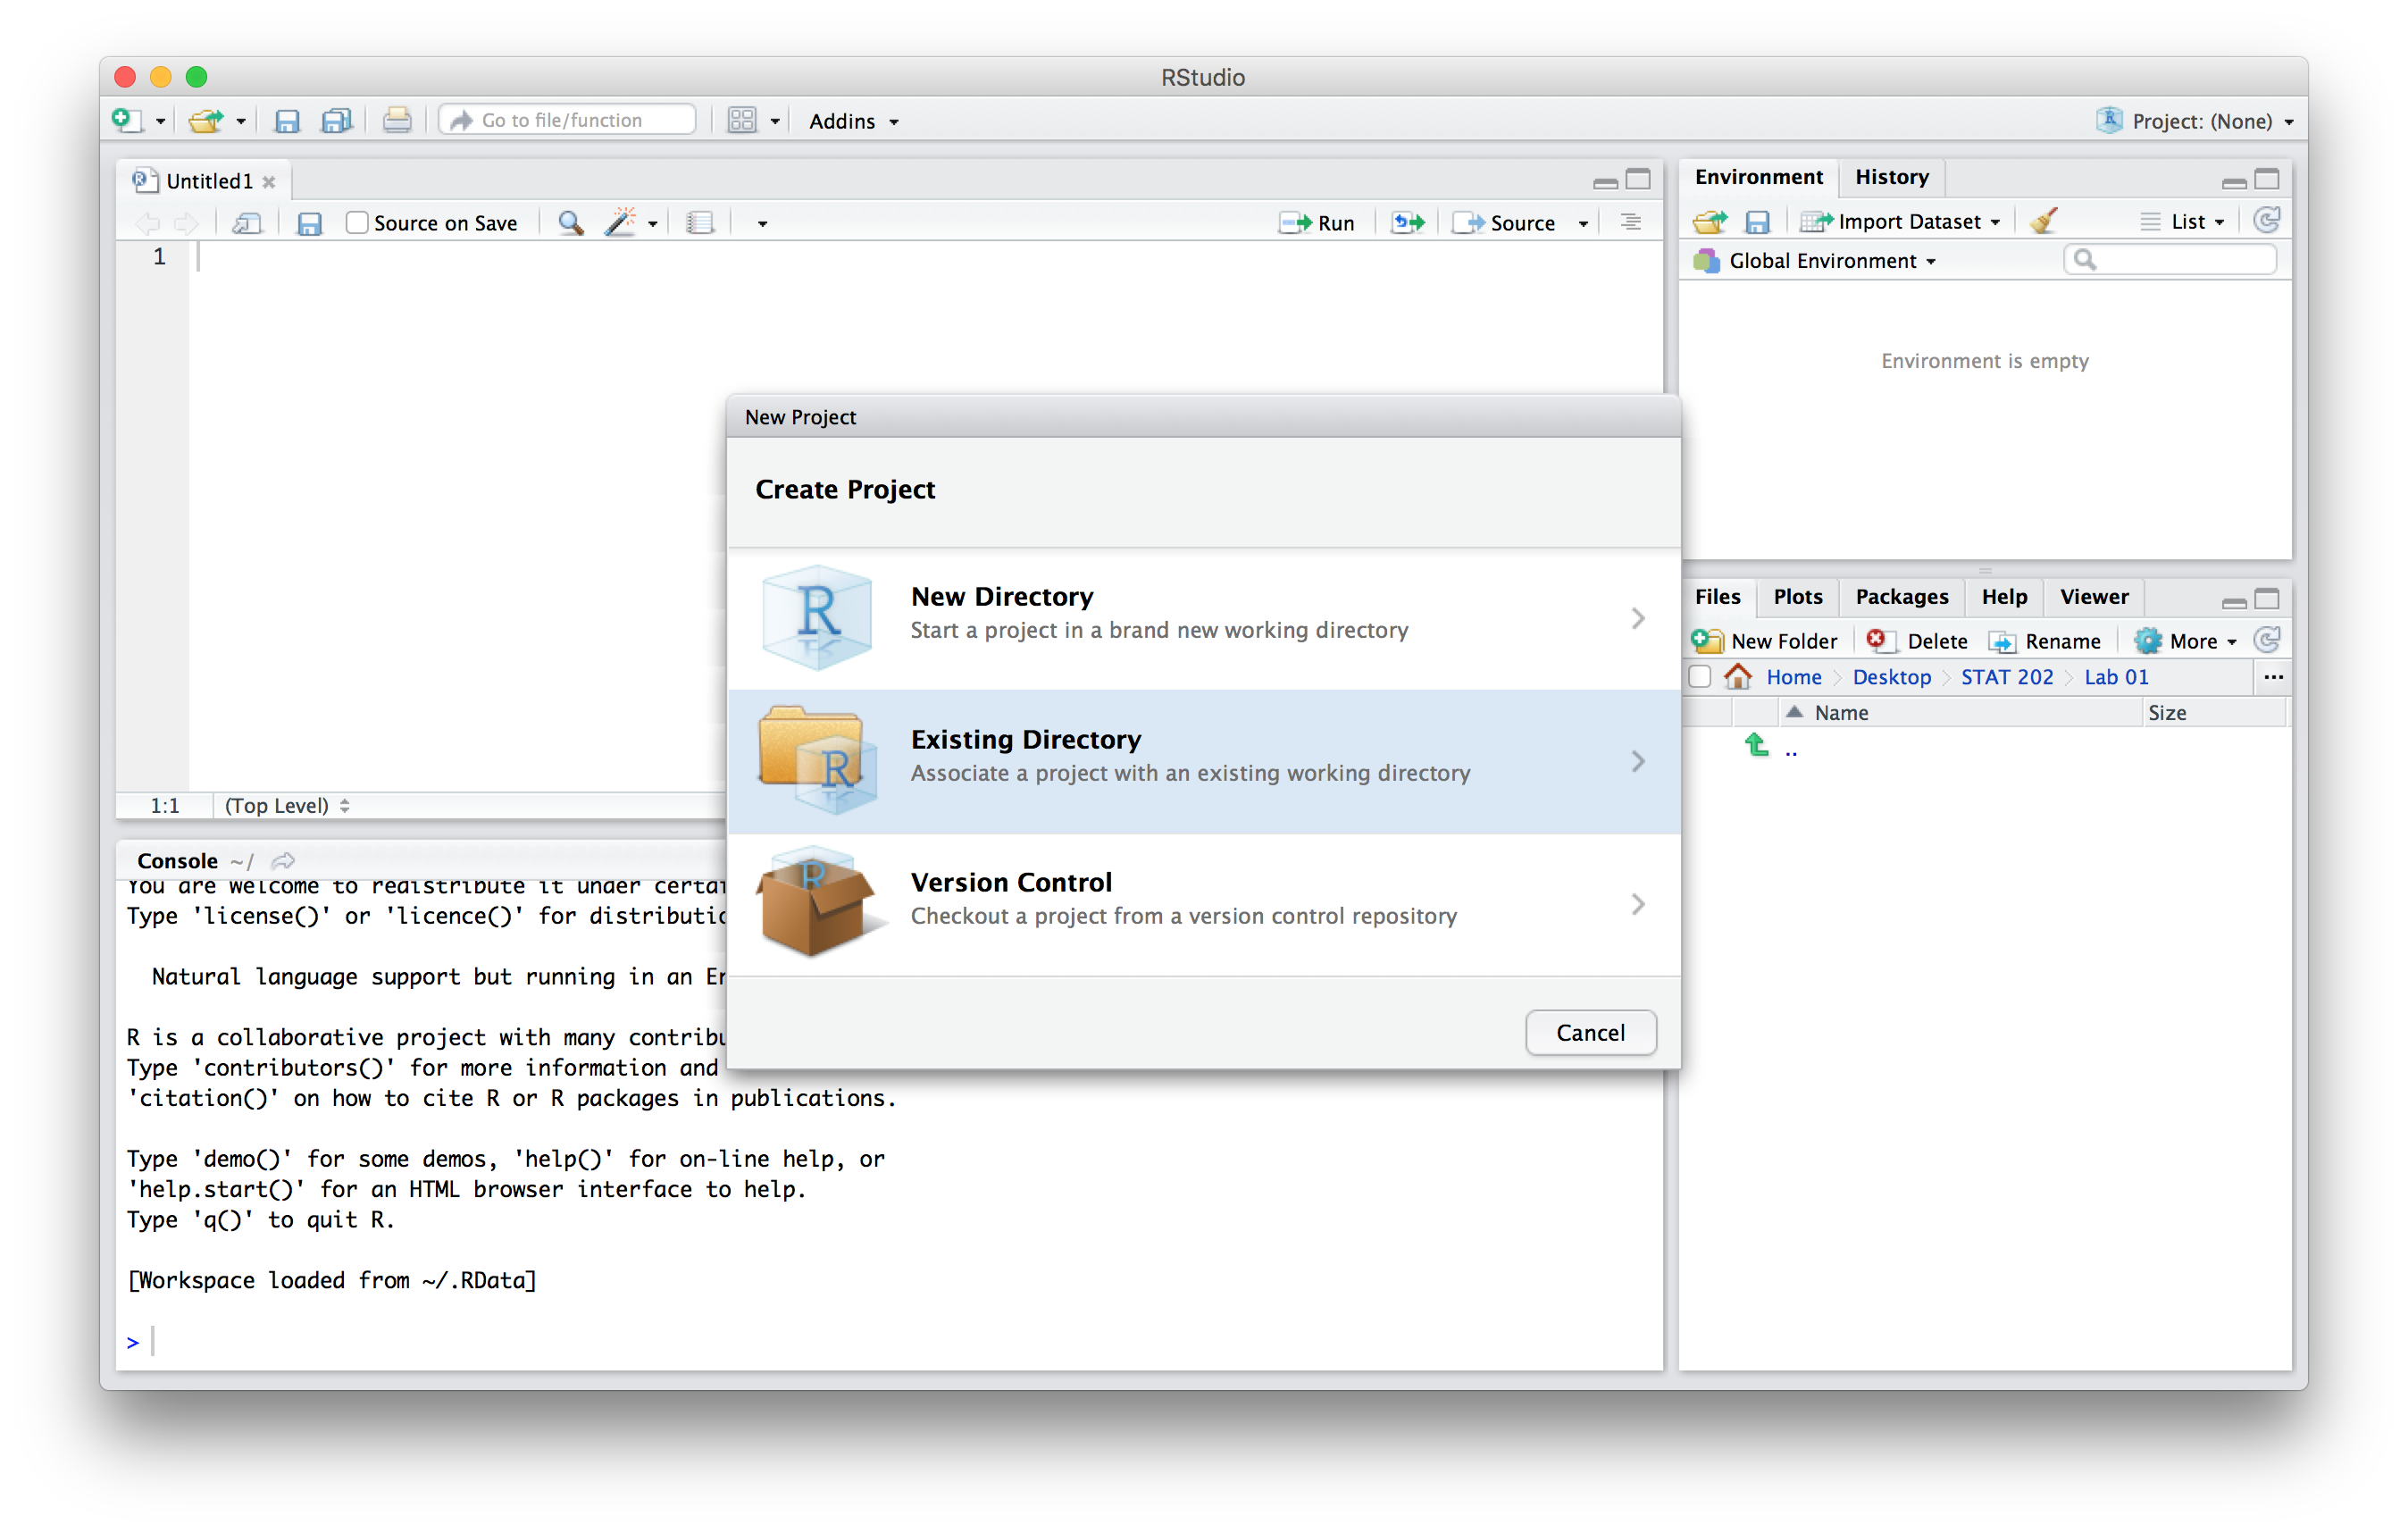
\includegraphics{./assets/images/01-03.png}
\caption{}
\end{figure}

\textbf{Step 6}

Click \textbf{Browse} and navigate to where you created the \textbf{Lab
01} folder. Select this folder and then click \textbf{Create Project}.

\begin{figure}[htbp]
\centering
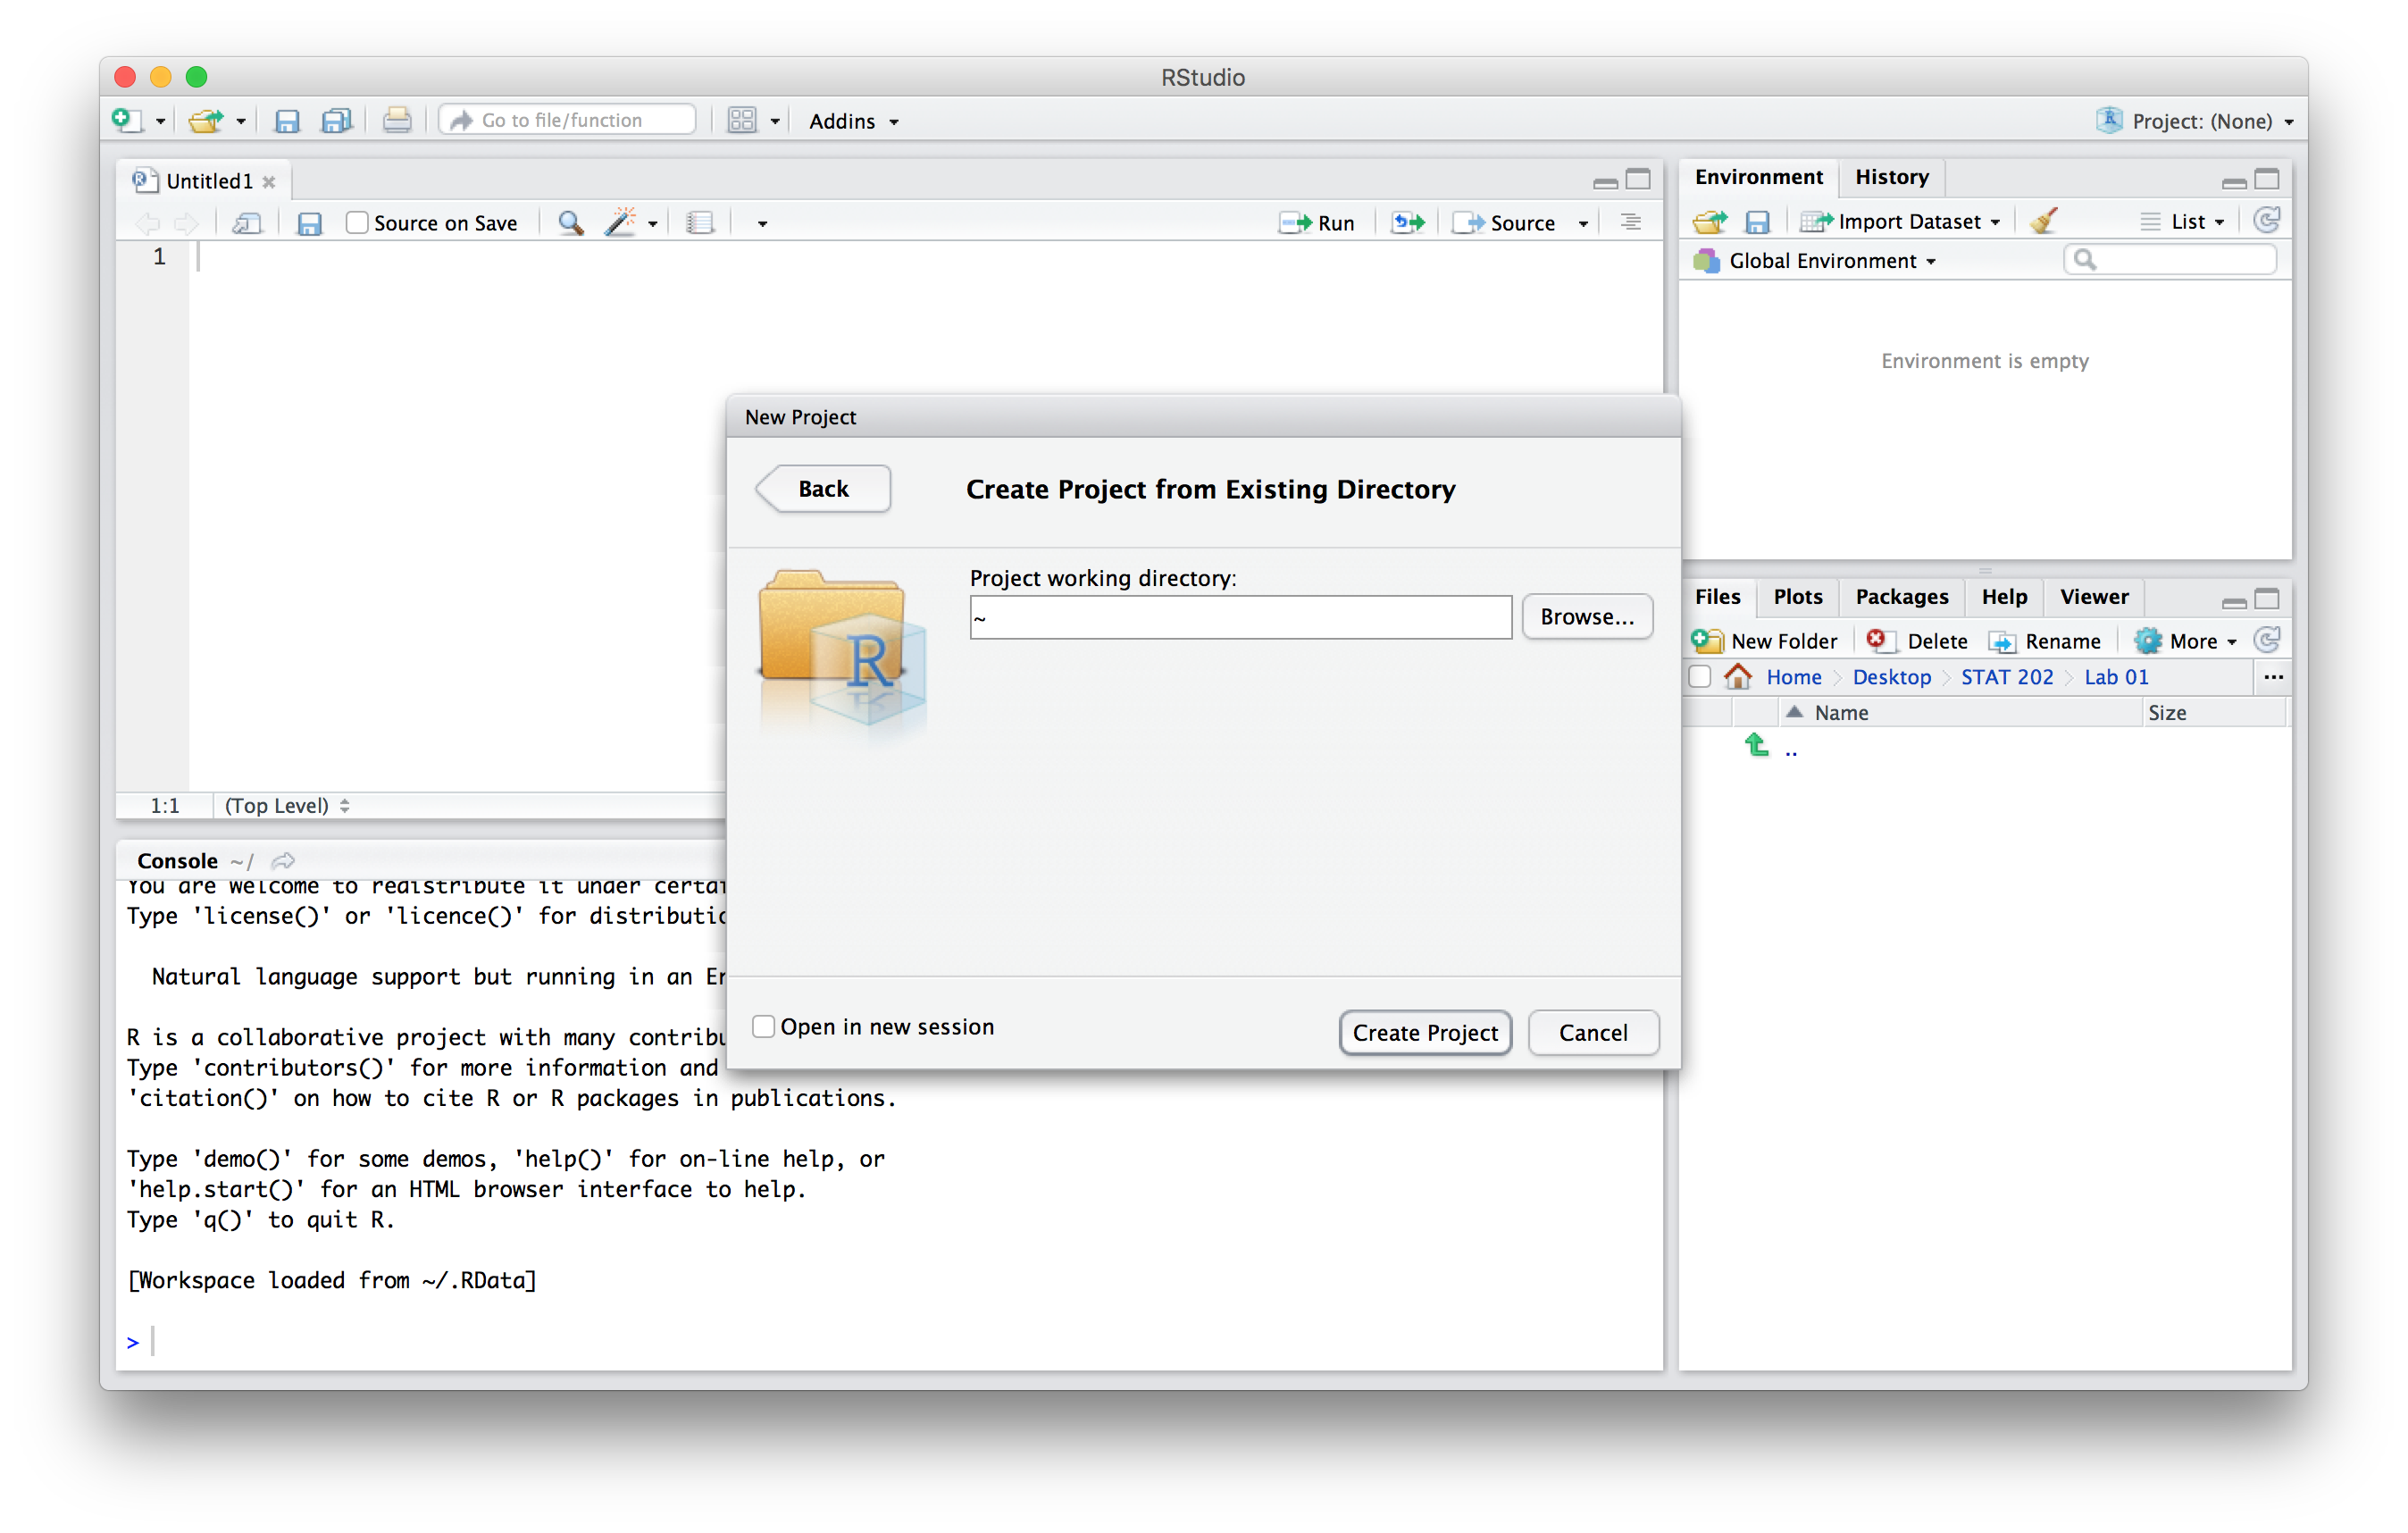
\includegraphics{./assets/images/01-04.png}
\caption{}
\end{figure}

Your R project has now been created. Note that in the upper right-hand
corner, the program indicates that you are working on the project named
\textbf{Lab 01}.

\begin{figure}[htbp]
\centering
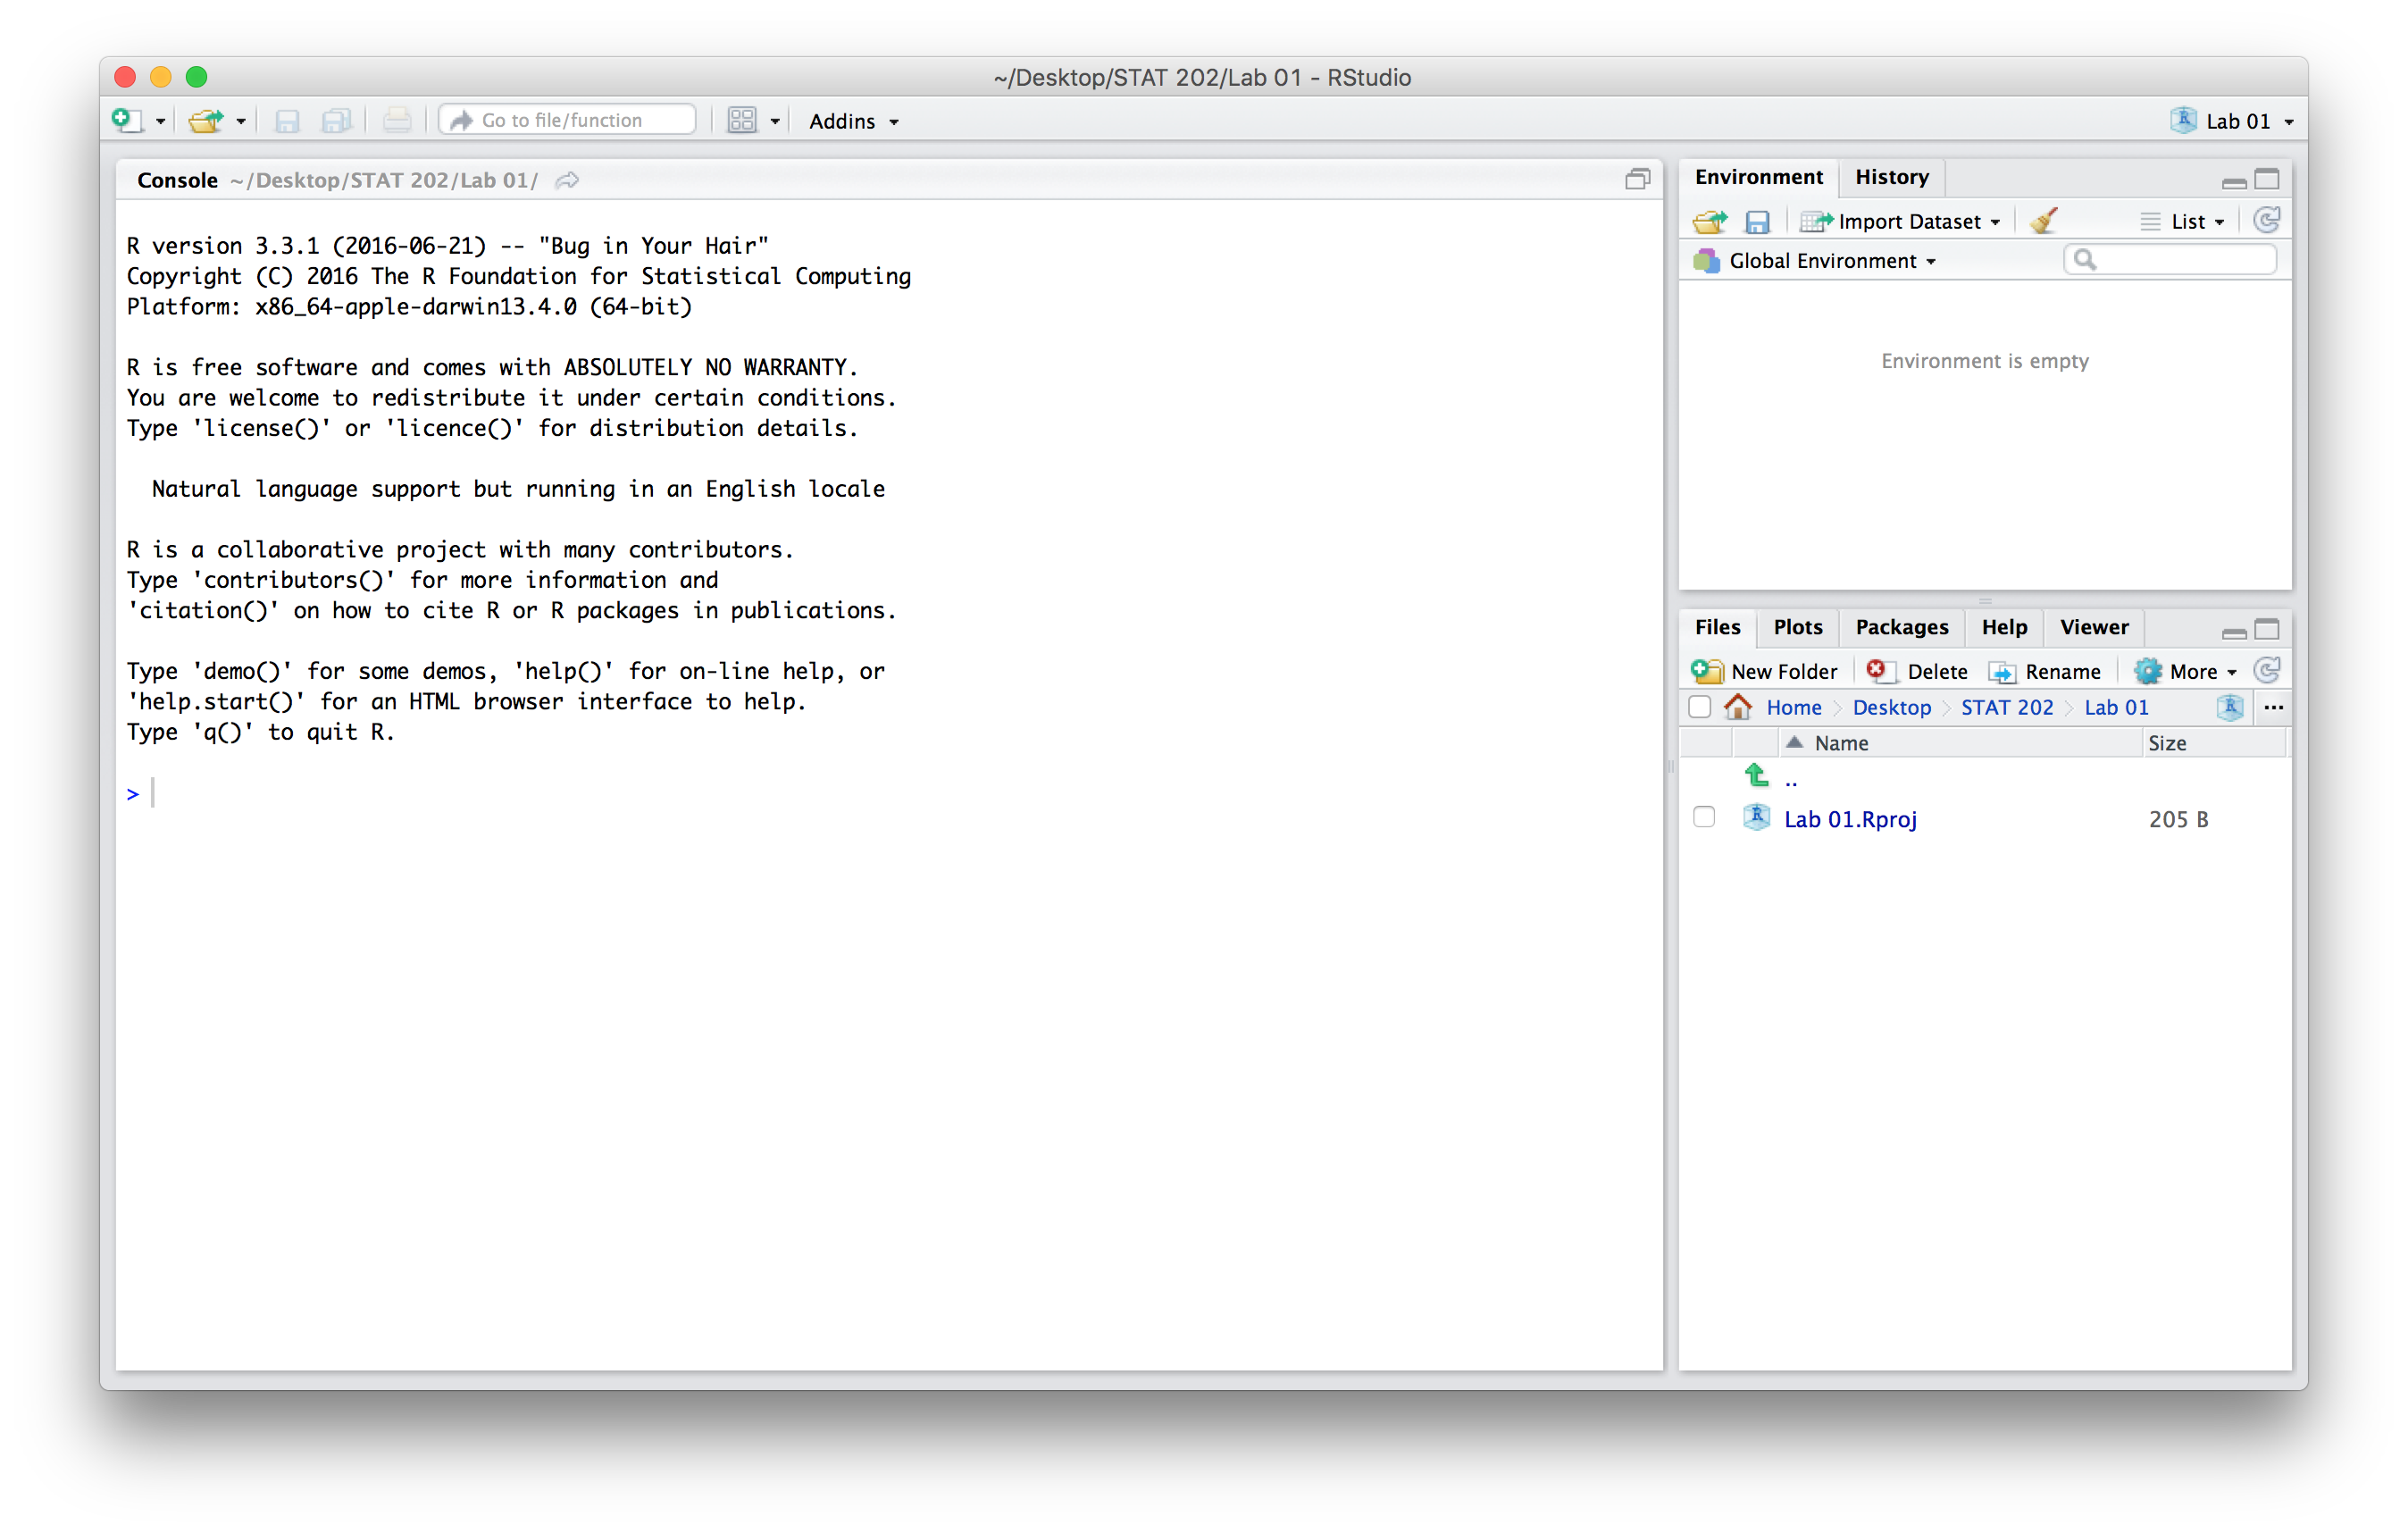
\includegraphics{./assets/images/01-05.png}
\caption{}
\end{figure}

\textbf{Step 7}

Creating an R script is the next MAJOR step in this process. Using a
script file is key to organizing your code for quick reference. You
should think of an R script file as a thorough record of how to conduct
an analysis or solve the problem at hand. You should strive to make your
R script as organized as possible so that someone else could work
through your code and reproduce the same output/answers/results.

To create an R script, go to the upper left-hand corner and click the
white box icon then select \textbf{R Script}.

\begin{figure}[htbp]
\centering
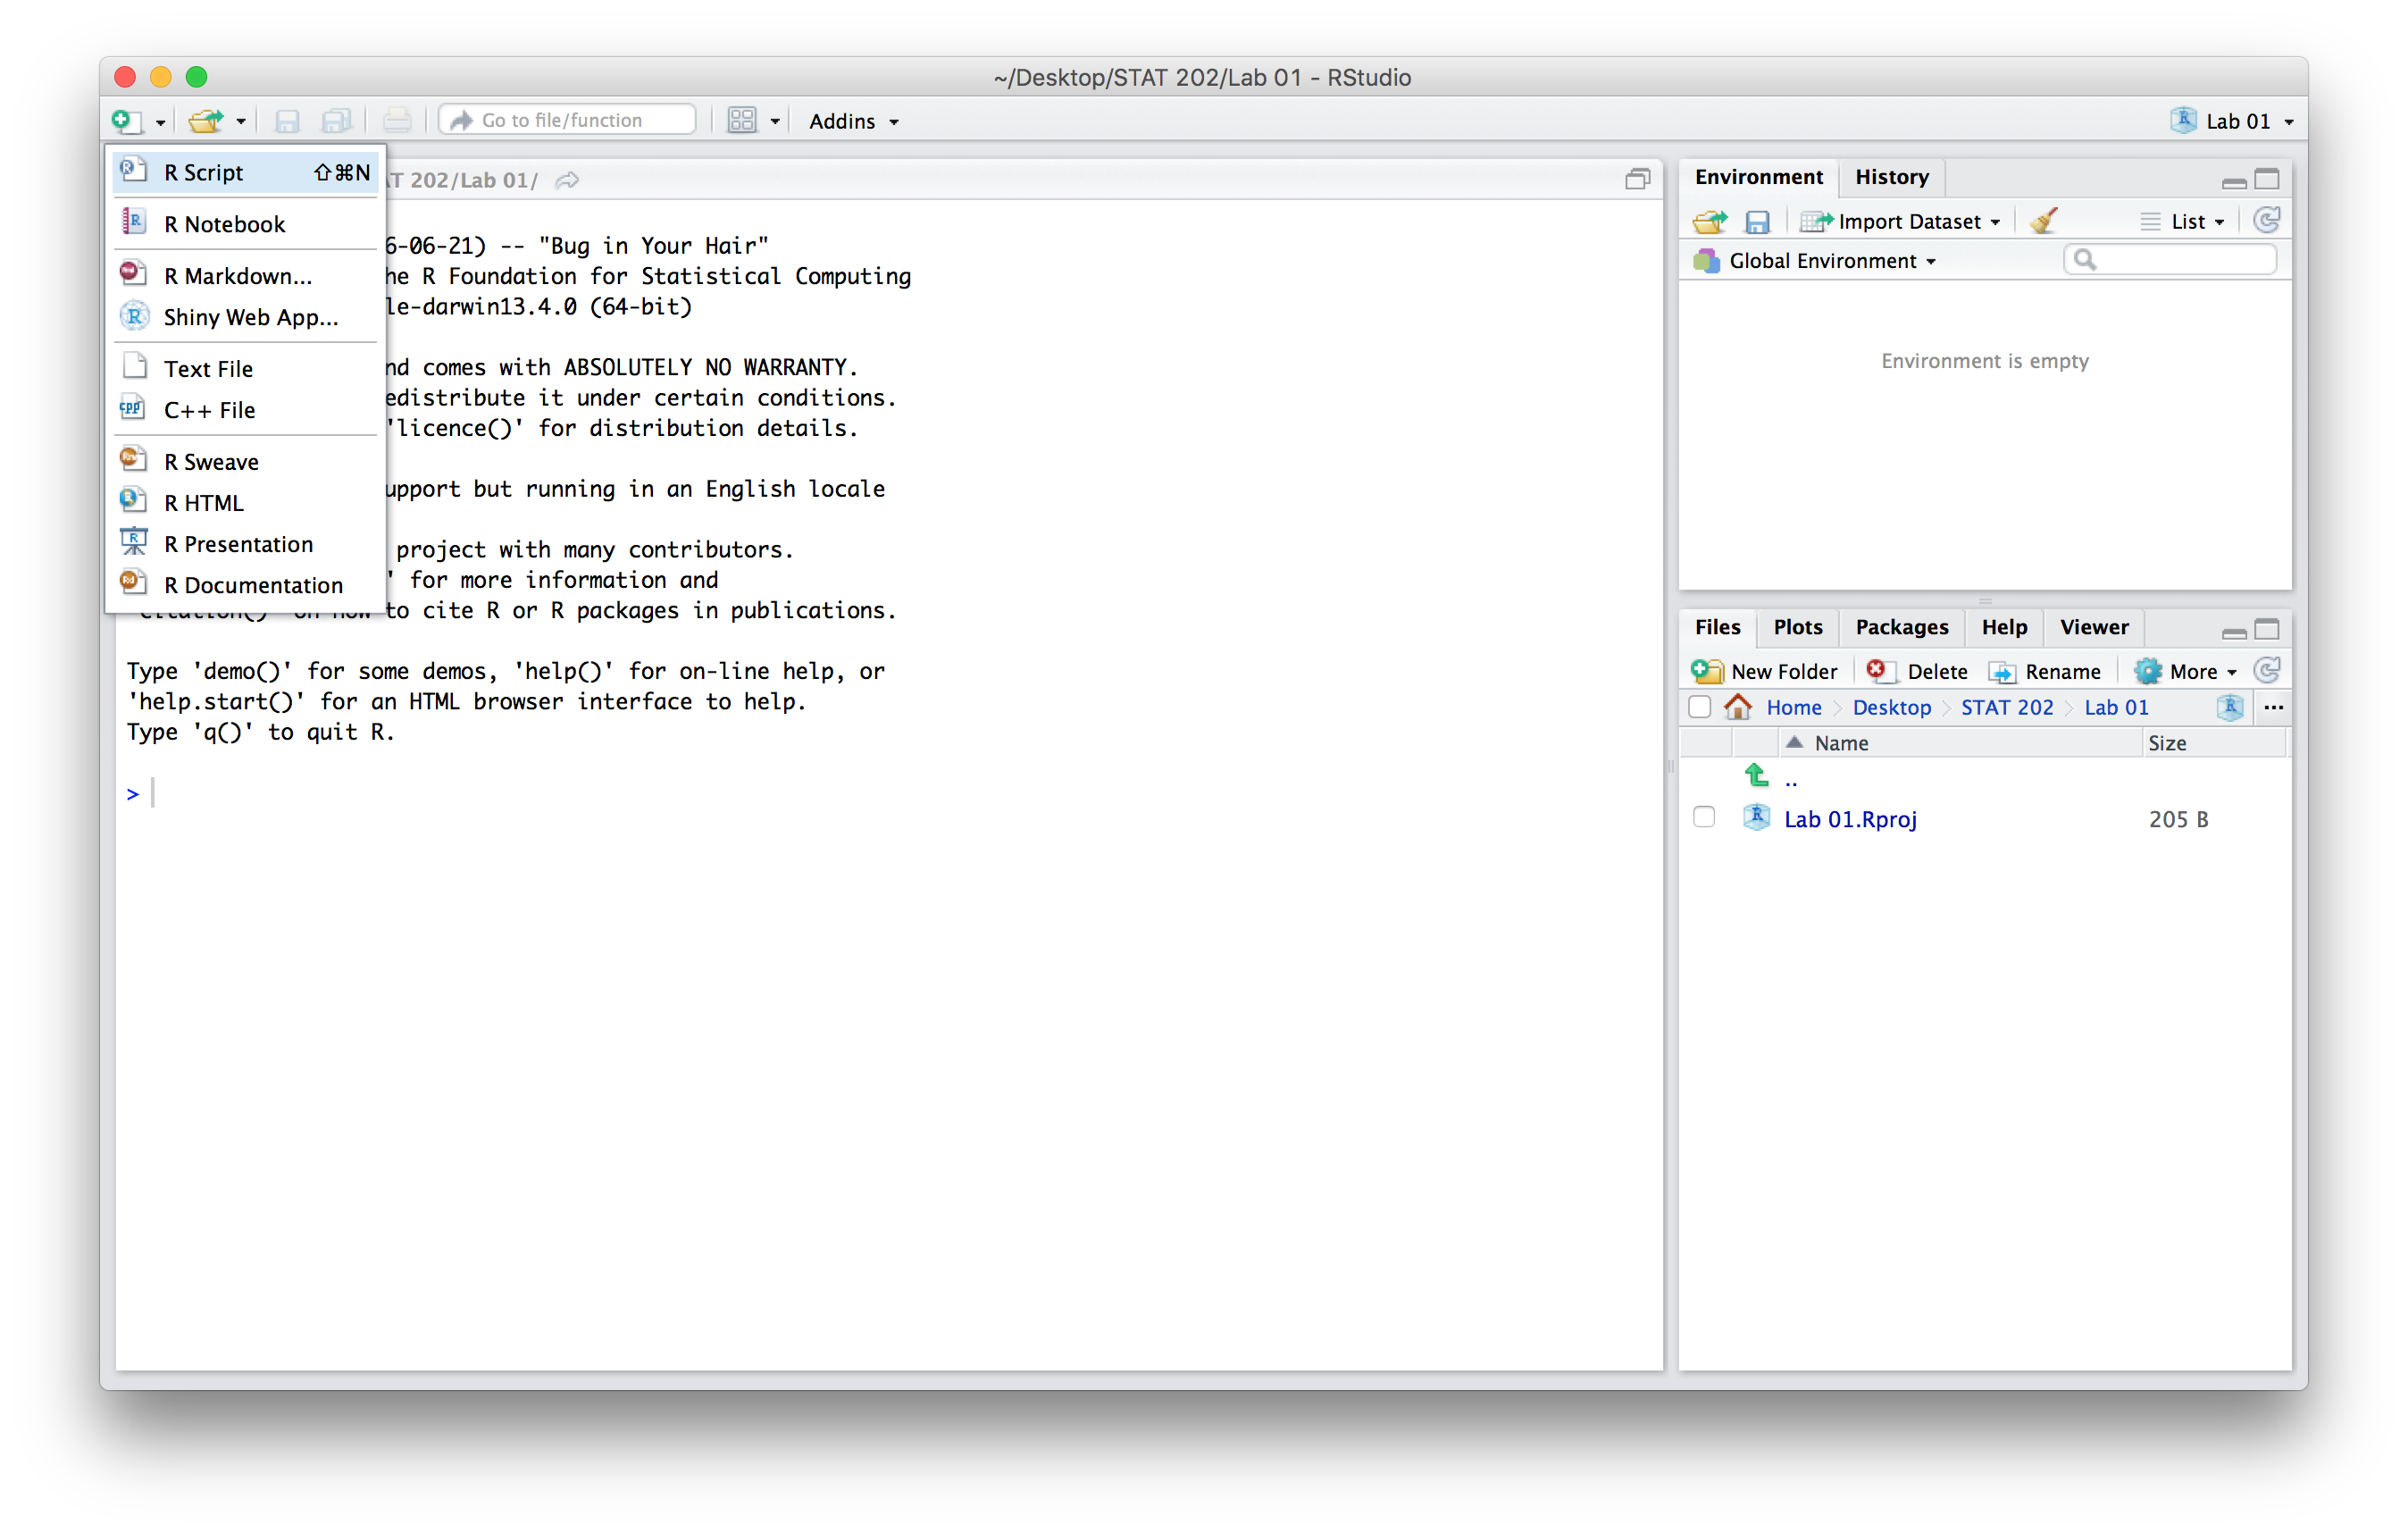
\includegraphics{./assets/images/01-06.png}
\caption{}
\end{figure}

\textbf{Step 8}

Now you can proceed to write your code in the R Script. You can also
save your progress by clicking on the save icon located in the icon bar.
Notice that it is saved within your R project folder --- \textbf{Lab 01}
in this case. This is why we created an R project, so that all of our
work for an analysis/project is kept in one central location.

Now, let's practice writing some R code. Good analytic code requires
good comments. Comments are meant for human consumption and to explain
what the executable code is doing. Therefore we need to let the program
know that it is a comment and that it should not attempt to run it. In
R, \texttt{\#} is used to signal a comment. In RStudio, this will turn
the line green, which indicates that it will be read as a comment ---
see the figure below. Also notice how we use white space (empty lines)
to make it easier on our eyes to navigate and read the script file.
\textbf{Practice by typying the code that is pictured.}

We can use R as a calculator, as shown below. To run the line of code
\texttt{2+2}, you place your cursor anywhere on the that line of code
and click \textbf{Run}, which is located in the top right corner of the
script pane. Alternatively, you could have used the keyboard short cut
of \textbf{Command + return} (Mac) or \textbf{ctrl + enter} (PC).

You also have the option of running multiple lines of code by
highlighting the lines of code and clicking \textbf{Run} or using the
keyboard short cut.

After running the command, the result will show up in your Console pane,
which is located beneath the Script pane. In the screenshot below, you
can see that our \texttt{2+2} command has generated an answer of
\texttt{4}.

\begin{figure}[htbp]
\centering
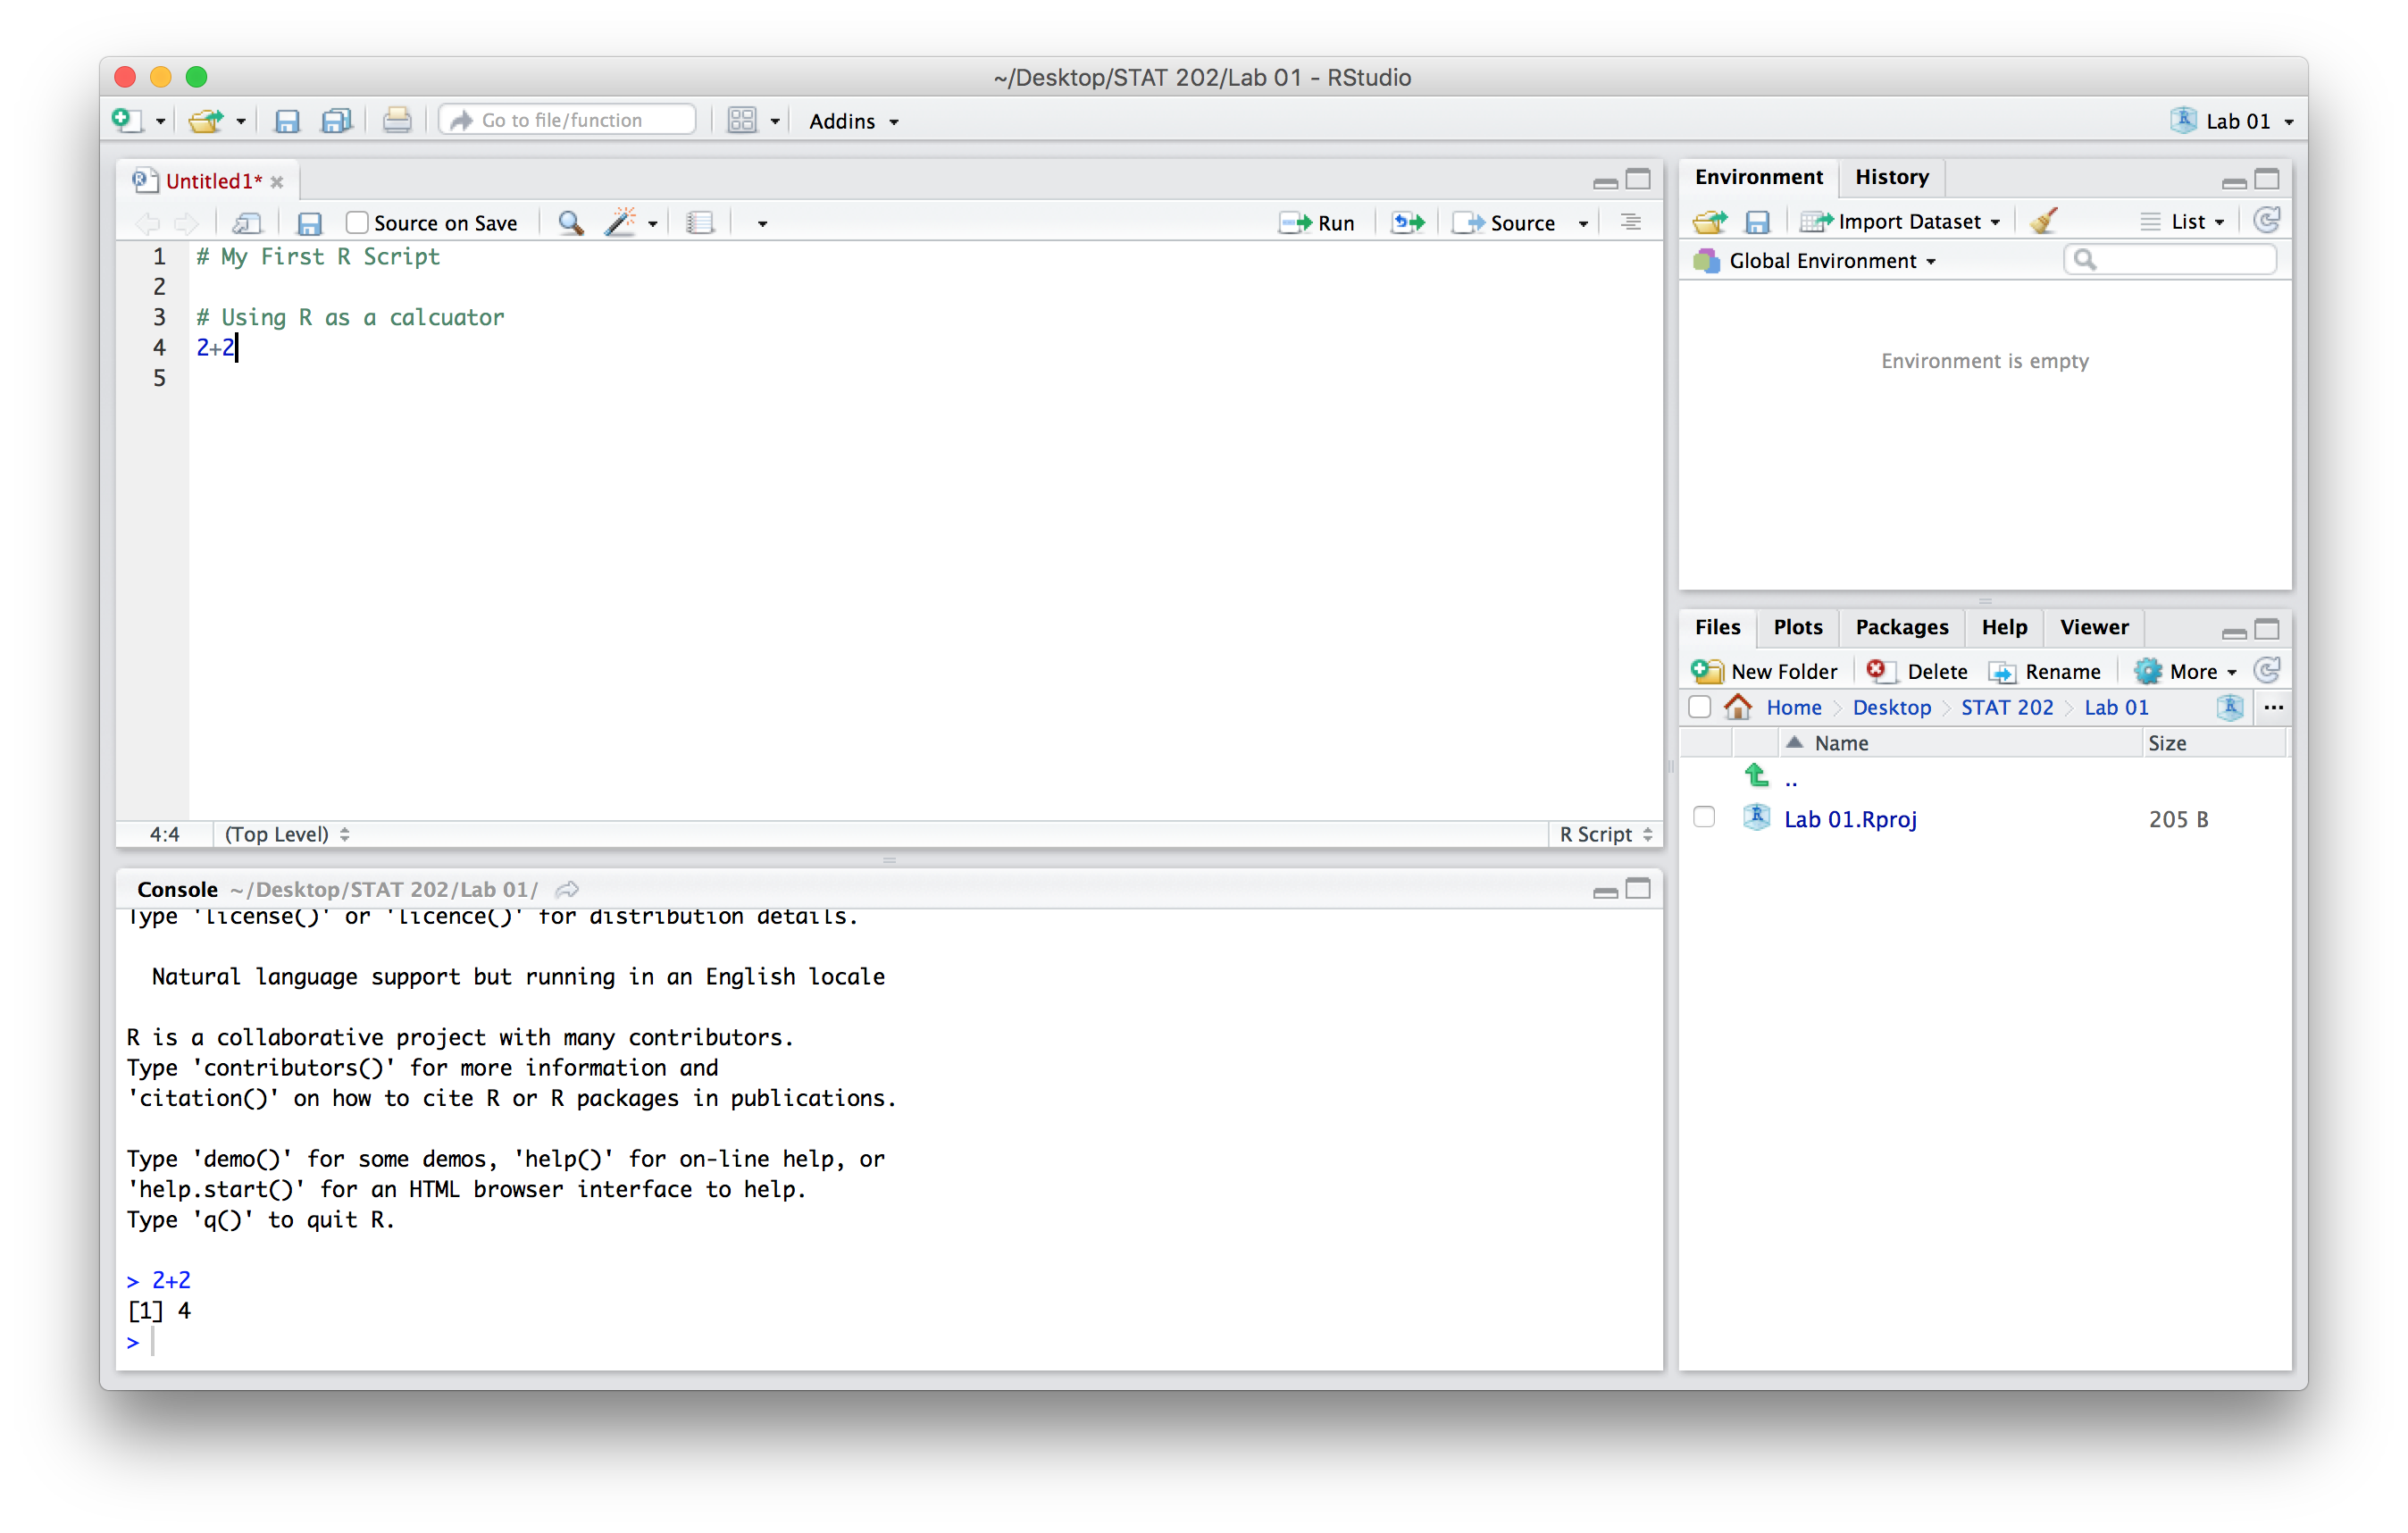
\includegraphics{./assets/images/01-07.png}
\caption{}
\end{figure}

Continue to practice writting an R script by reproducing the code
depicted below. As the comments in the pictured code indicate, we are
loading/reading-in the \texttt{arbuthnot} dataset. Then we are taking a
look at some of the observations from the dataset by using the functions
\texttt{head()} and \texttt{tail()}. Make sure to run the lines of code
in order, otherwise the the software will return error messages. We
suggest running one line at a time to ensure your code is typed
correctly and to see what each line is doing.

\begin{figure}[htbp]
\centering
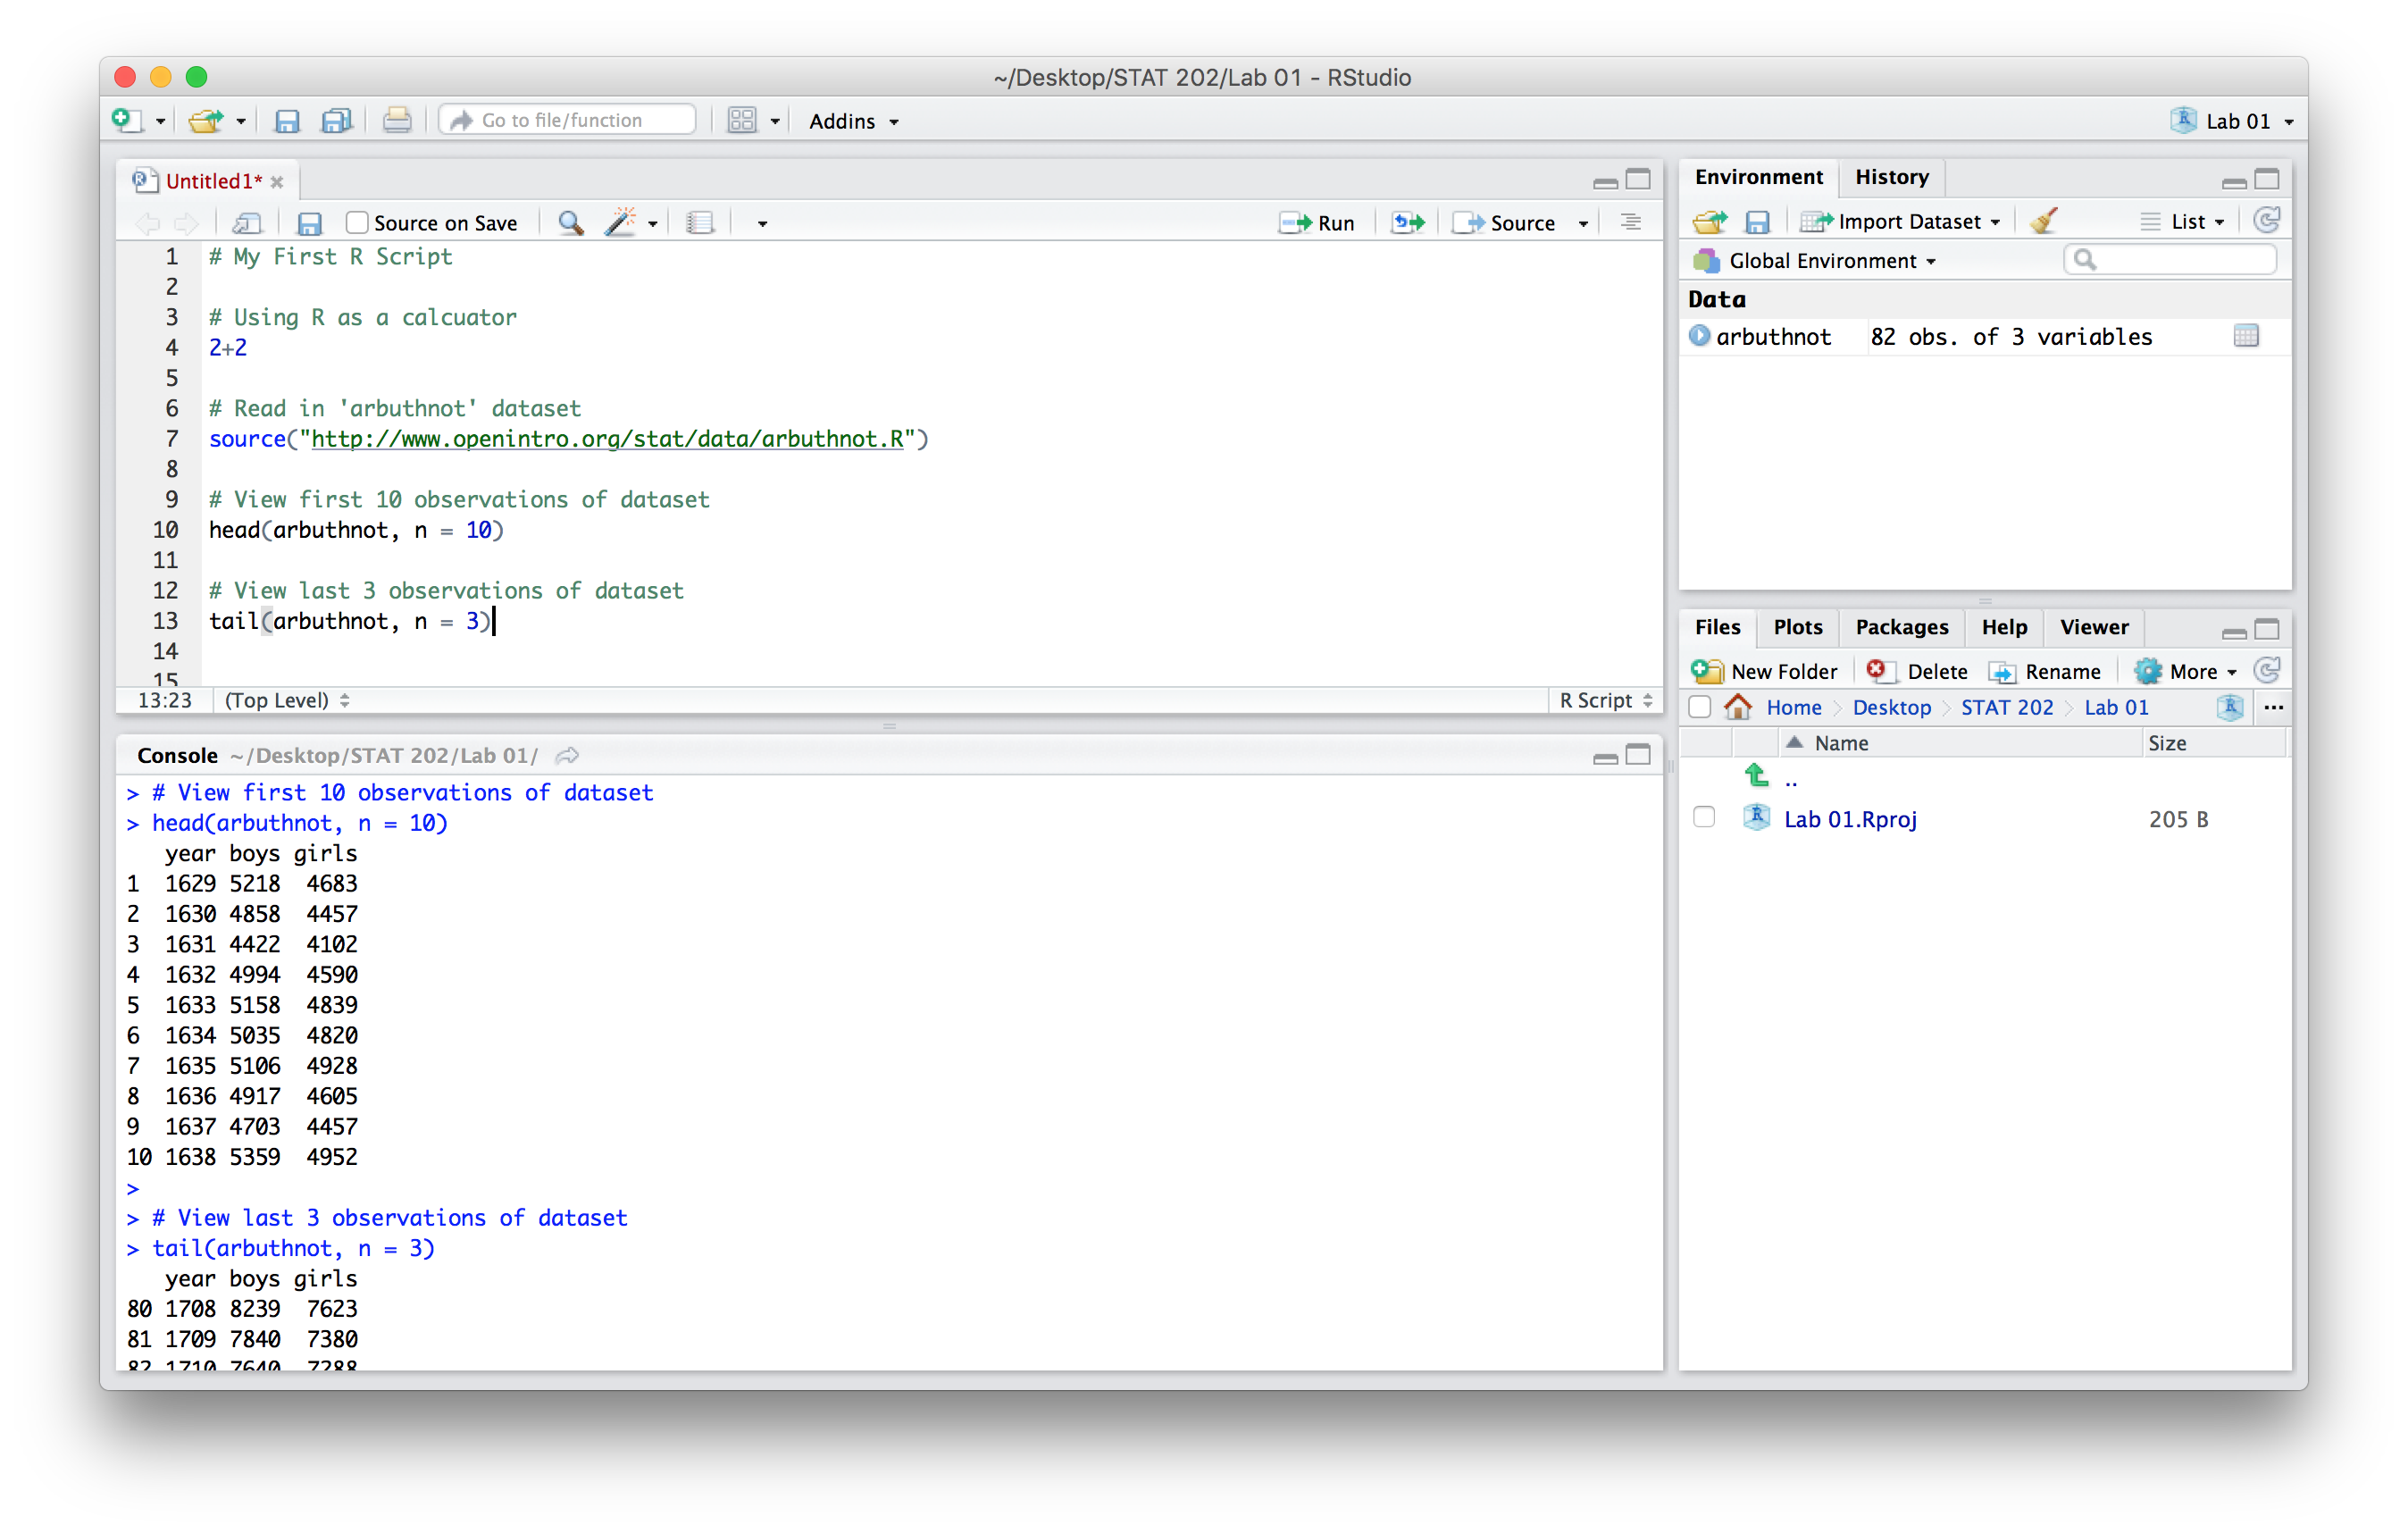
\includegraphics{./assets/images/01-08.png}
\caption{}
\end{figure}

Notice the copious usage of comments in our analytic code. In general,
analytic code should make liberal use of comments. The length and
specificity of comments depends on a person's experience with a coding
language. With experience comes the understanding and ability to write
concise comments that cut directly to what information is absolutely
necessary to communicate. It never hurts to have more comments than
actual executable code, especially for those new to coding. Keep in mind
that in the future you might want to share analytic code with co-workers
or peers, or go back to reference code months or years after you've
written it.

\begin{center}\rule{0.5\linewidth}{\linethickness}\end{center}

\section{Summary}\label{summary}

The essential workflow that should be followed for each lab:

\begin{enumerate}
\def\labelenumi{\arabic{enumi}.}
\tightlist
\item
  Create and work in an R project to ensure all work is kept in a single
  location.
\item
  Organize your work within an R script.

  \begin{itemize}
  \tightlist
  \item
    Use comments to clearly communicate what the code is doing.
  \item
    Use white space (empty lines and spaces) to make the document easier
    to read and navigate.
  \end{itemize}
\end{enumerate}

There are many other features of RStudio that you'll find useful, but
are not covered in this document. RStudio strives to provide help in
many different ways:

\begin{enumerate}
\def\labelenumi{\arabic{enumi}.}
\tightlist
\item
  The help tab within the lower right-hand pane.
\item
  Help automatically appears when typing a function (auto-complete).
\item
  You may begin by typing the name of function and it will suggest
  several options.
\end{enumerate}

\chapter{Introduction to R and
RStudio}\label{introduction-to-r-and-rstudio}

The goal of this lab is to introduce you to R and RStudio, which you'll
be using throughout the course both to learn the statistical concepts
discussed in the
\href{https://www.openintro.org/stat/textbook.php}{texbook} and also to
analyze real data and come to informed conclusions. To straighten out
which is which: R is the name of \emph{the programming language} itself
and RStudio is a convenient \emph{user interface} for working with R.

As the labs progress, you are encouraged to explore beyond what the labs
dictate; a willingness to experiment will make you a much better
programmer. Before we get to that stage, however, you need to build some
basic fluency in R. Today we begin with the fundamental building blocks
of R and RStudio: the interface, reading in data, and basic commands.

\begin{figure}[htbp]
\centering
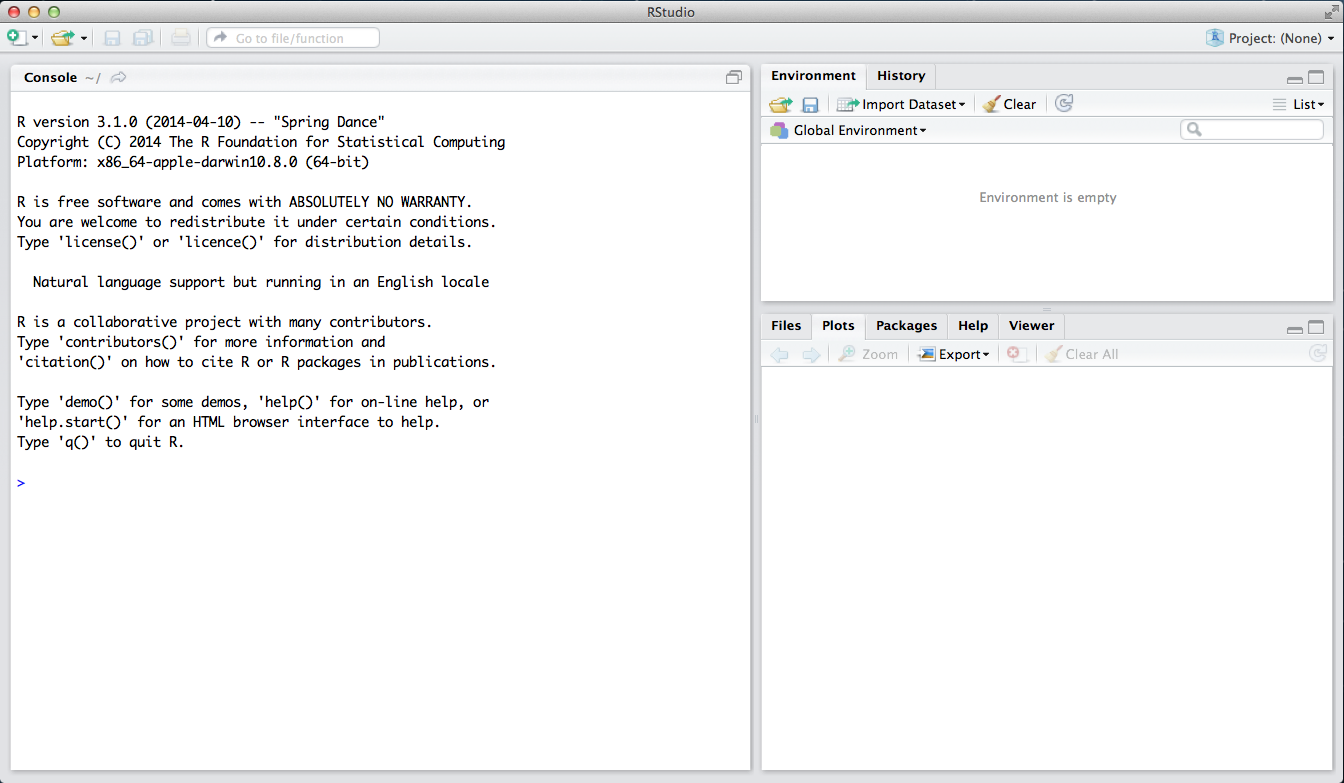
\includegraphics{./assets/images/02-01.png}
\caption{The RStudio Interface}
\end{figure}

The panel in the upper right contains your \emph{workspace} as well as a
history of the commands that you've previously entered. Any plots that
you generate will show up in the panel in the lower right corner.

The panel on the left is where the action happens. It's called the
\emph{console}. Everytime you launch RStudio, it will have the same text
at the top of the console telling you the version of R that you're
running. Below that information is the \emph{prompt}. As its name
suggests, this prompt is really a request, a request for a command.
Initially, interacting with R is all about typing commands and
interpreting the output. These commands and their syntax have evolved
over decades (literally) and now provide what many users feel is a
fairly natural way to access data and organize, describe, and invoke
statistical computations.

To get you started, enter the following command at the R prompt
(i.e.~right after \texttt{\textgreater{}} on the console). You can
either type it in manually or copy and paste it from this document.

\begin{Shaded}
\begin{Highlighting}[]
\KeywordTok{source}\NormalTok{(}\StringTok{"http://www.openintro.org/stat/data/arbuthnot.R"}\NormalTok{)}
\end{Highlighting}
\end{Shaded}

This command instructs R to access the OpenIntro website and fetch some
data: the Arbuthnot baptism counts for boys and girls. You should see
that the workspace area in the upper righthand corner of the RStudio
window now lists a data set called \texttt{arbuthnot} that has 82
observations on 3 variables. As you interact with R, you will create a
series of objects. Sometimes you load them as we have done here, and
sometimes you create them yourself as the byproduct of a computation or
some analysis you have performed. Note that because you are accessing
data from the web, this command (and the entire assignment) will work in
a computer lab, in the library, or in your dorm room; anywhere you have
access to the Internet.

\section{The Data: Dr.~Arbuthnot's Baptism
Records}\label{the-data-dr.arbuthnots-baptism-records}

The Arbuthnot data set refers to Dr.~John Arbuthnot, an 18th century
physician, writer, and mathematician. He was interested in the ratio of
newborn boys to newborn girls, so he gathered the baptism records for
children born in London for every year from 1629 to 1710. We can take a
look at the data by typing its name into the console.

\begin{Shaded}
\begin{Highlighting}[]
\NormalTok{arbuthnot}
\end{Highlighting}
\end{Shaded}

What you should see are four columns of numbers, each row representing a
different year: the first entry in each row is simply the row number (an
index we can use to access the data from individual years if we want),
the second is the year, and the third and fourth are the numbers of boys
and girls baptized that year, respectively. Use the scrollbar on the
right side of the console window to examine the complete data set.

Note that the row numbers in the first column are not part of
Arbuthnot's data. R adds them as part of its printout to help you make
visual comparisons. You can think of them as the index that you see on
the left side of a spreadsheet. In fact, the comparison to a spreadsheet
will generally be helpful. R has stored Arbuthnot's data in a kind of
spreadsheet or table called a \emph{data frame}.

You can see the dimensions of this data frame by typing:

\begin{Shaded}
\begin{Highlighting}[]
\KeywordTok{dim}\NormalTok{(arbuthnot)}
\end{Highlighting}
\end{Shaded}

\begin{verbatim}
## [1] 82  3
\end{verbatim}

This command should output \texttt{{[}1{]}\ 82\ 3}, indicating that
there are 82 rows and 3 columns (we'll get to what the \texttt{{[}1{]}}
means in a bit), just as it says next to the object in your workspace.
You can see the names of these columns (or variables) by typing:

\begin{Shaded}
\begin{Highlighting}[]
\KeywordTok{names}\NormalTok{(arbuthnot)}
\end{Highlighting}
\end{Shaded}

\begin{verbatim}
## [1] "year"  "boys"  "girls"
\end{verbatim}

You should see that the data frame contains the columns \texttt{year},
\texttt{boys}, and \texttt{girls}. At this point, you might notice that
many of the commands in R look a lot like functions from math class;
that is, invoking R commands means supplying a function with some number
of arguments. The \texttt{dim} and \texttt{names} commands, for example,
each took a single argument, the name of a data frame.

One advantage of RStudio is that it comes with a built-in data viewer.
Click on the name \texttt{arbuthnot} in the \emph{Environment} pane
(upper right window) that lists the objects in your workspace. This will
bring up an alternative display of the data set in the \emph{Data
Viewer} (upper left window). You can close the data viewer by clicking
on the \emph{x} in the upper lefthand corner.

\section{Some Exploration}\label{some-exploration}

Let's start to examine the data a little more closely. We can access the
data in a single column of a data frame separately using a command like

\begin{Shaded}
\begin{Highlighting}[]
\NormalTok{arbuthnot$boys}
\end{Highlighting}
\end{Shaded}

This command will only show the number of boys baptized each year.

\begin{center}\rule{0.5\linewidth}{\linethickness}\end{center}

\textbf{Excercise 1:} What command would you use to extract just the
counts of girls baptized? Try it!

\begin{center}\rule{0.5\linewidth}{\linethickness}\end{center}

Notice that the way R has printed these data is different. When we
looked at the complete data frame, we saw 82 rows, one on each line of
the display. These data are no longer structured in a table with other
variables, so they are displayed one right after another. Objects that
print out in this way are called \emph{vectors}; they represent a set of
numbers. R has added numbers in {[}brackets{]} along the left side of
the printout to indicate locations within the vector. For example,
\texttt{5218} follows \texttt{{[}1{]}}, indicating that \texttt{5218} is
the first entry in the vector. And if \texttt{{[}43{]}} starts a line,
then that would mean the first number on that line would represent the
43rd entry in the vector.

R has some powerful functions for making graphics. We can create a
simple plot of the number of girls baptized per year with the command:

\begin{Shaded}
\begin{Highlighting}[]
\KeywordTok{plot}\NormalTok{(}\DataTypeTok{x =} \NormalTok{arbuthnot$year, }\DataTypeTok{y =} \NormalTok{arbuthnot$girls)}
\end{Highlighting}
\end{Shaded}

By default, R creates a scatterplot with each x,y pair indicated by an
open circle. The plot itself should appear under the \emph{Plots} tab of
the lower right panel of RStudio. Notice that the command above again
looks like a function, this time with two arguments separated by a
comma. The first argument in the plot function specifies the variable
for the x-axis and the second for the y-axis. If we wanted to connect
the data points with lines, we could add a third argument, the letter
\texttt{l} for line.

\begin{Shaded}
\begin{Highlighting}[]
\KeywordTok{plot}\NormalTok{(}\DataTypeTok{x =} \NormalTok{arbuthnot$year, }\DataTypeTok{y =} \NormalTok{arbuthnot$girls, }\DataTypeTok{type =} \StringTok{"l"}\NormalTok{)}
\end{Highlighting}
\end{Shaded}

You might wonder how you are supposed to know that it was possible to
add that third argument. Thankfully, R documents all of its functions
extensively. To read what a function does and learn the arguments that
are available to you, just type in a question mark followed by the name
of the function that you're interested in. Try the following.

\begin{Shaded}
\begin{Highlighting}[]
\NormalTok{?plot}
\end{Highlighting}
\end{Shaded}

Notice that the help file replaces the plot in the lower right panel.
You can toggle between plots and help files using the tabs at the top of
that panel.

\begin{center}\rule{0.5\linewidth}{\linethickness}\end{center}

\textbf{Exercise 2:} Is there an apparent trend in the number of girls
baptized over the years? How would you describe it?

\begin{center}\rule{0.5\linewidth}{\linethickness}\end{center}

Now, suppose we want to plot the total number of baptisms. To compute
this, we could use the fact that R is really just a big calculator. We
can type in mathematical expressions like

\begin{Shaded}
\begin{Highlighting}[]
\DecValTok{5218} \NormalTok{+}\StringTok{ }\DecValTok{4683}
\end{Highlighting}
\end{Shaded}

to see the total number of baptisms in 1629. We could repeat this once
for each year, but there is a faster way. If we add the vector for
baptisms for boys and girls, R will compute all sums simultaneously.

\begin{Shaded}
\begin{Highlighting}[]
\NormalTok{arbuthnot$boys +}\StringTok{ }\NormalTok{arbuthnot$girls}
\end{Highlighting}
\end{Shaded}

What you will see are 82 numbers (in that packed display, because we
aren't looking at a data frame here), each one representing the sum
we're after. Take a look at a few of them and verify that they are
right. Therefore, we can make a plot of the total number of baptisms per
year with the command

\begin{Shaded}
\begin{Highlighting}[]
\KeywordTok{plot}\NormalTok{(arbuthnot$year, arbuthnot$boys +}\StringTok{ }\NormalTok{arbuthnot$girls, }\DataTypeTok{type =} \StringTok{"l"}\NormalTok{)}
\end{Highlighting}
\end{Shaded}

This time, note that we left out the names of the first two arguments.
We can do this because the help file shows that the default for
\texttt{plot} is for the first argument to be the x-variable and the
second argument to be the y-variable.

Similarly to how we computed the proportion of boys, we can compute the
ratio of the number of boys to the number of girls baptized in 1629 with

\begin{Shaded}
\begin{Highlighting}[]
\DecValTok{5218} \NormalTok{/}\StringTok{ }\DecValTok{4683}
\end{Highlighting}
\end{Shaded}

or we can act on the complete vectors with the expression

\begin{Shaded}
\begin{Highlighting}[]
\NormalTok{arbuthnot$boys /}\StringTok{ }\NormalTok{arbuthnot$girls}
\end{Highlighting}
\end{Shaded}

The proportion of newborns that are boys

\begin{Shaded}
\begin{Highlighting}[]
\DecValTok{5218} \NormalTok{/}\StringTok{ }\NormalTok{(}\DecValTok{5218} \NormalTok{+}\StringTok{ }\DecValTok{4683}\NormalTok{)}
\end{Highlighting}
\end{Shaded}

or this may also be computed for all years simultaneously:

\begin{Shaded}
\begin{Highlighting}[]
\NormalTok{arbuthnot$boys /}\StringTok{ }\NormalTok{(arbuthnot$boys +}\StringTok{ }\NormalTok{arbuthnot$girls)}
\end{Highlighting}
\end{Shaded}

Note that with R as with your calculator, you need to be conscious of
the order of operations. Here, we want to divide the number of boys by
the total number of newborns, so we have to use parentheses. Without
them, R will first do the division, then the addition, giving you
something that is not a proportion.

\begin{center}\rule{0.5\linewidth}{\linethickness}\end{center}

\textbf{Exercise 3:} Now, make a plot of the proportion of boys over
time. What do you see? Tip: If you use the up and down arrow keys, you
can scroll through your previous commands, your so-called command
history. You can also access it by clicking on the history tab in the
upper right panel. This will save you a lot of typing in the future.

\begin{center}\rule{0.5\linewidth}{\linethickness}\end{center}

Finally, in addition to simple mathematical operators like subtraction
and division, you can ask R to make comparisons like greater than,
\texttt{\textgreater{}}, less than, \texttt{\textless{}}, and equality,
\texttt{==}. For example, we can ask if boys outnumber girls in each
year with the expression

\begin{Shaded}
\begin{Highlighting}[]
\NormalTok{arbuthnot$boys >}\StringTok{ }\NormalTok{arbuthnot$girls}
\end{Highlighting}
\end{Shaded}

This command returns 82 values of either \texttt{TRUE} if that year had
more boys than girls, or \texttt{FALSE} if that year did not (the answer
may surprise you). This output shows a different kind of data than we
have considered so far. In the \texttt{arbuthnot} data frame our values
are numerical (the year, the number of boys and girls). Here, we've
asked R to create \emph{logical} data, data where the values are either
\texttt{TRUE} or \texttt{FALSE}. In general, data analysis will involve
many different kinds of data types, and one reason for using R is that
it is able to represent and compute with many of them.

This seems like a fair bit for your first lab, so let's stop here. To
exit RStudio you can click the \emph{x} in the upper right corner of the
whole window. You will be prompted to save your workspace. If you click
\emph{save}, RStudio will save the history of your commands and all the
objects in your workspace so that the next time you launch RStudio, you
will see \texttt{arbuthnot} and you will have access to the commands you
typed in your previous session. For now, click \emph{save}, then start
up RStudio again.

\begin{center}\rule{0.5\linewidth}{\linethickness}\end{center}

\section{On Your Own}\label{on-your-own}

In the previous few pages, you recreated some of the displays and
preliminary analysis of Arbuthnot's baptism data. Your assignment
involves repeating these steps, but for present day birth records in the
United States. Load up the present day data with the following command.

\begin{Shaded}
\begin{Highlighting}[]
\KeywordTok{source}\NormalTok{(}\StringTok{"http://www.openintro.org/stat/data/present.R"}\NormalTok{)}
\end{Highlighting}
\end{Shaded}

The data are stored in a data frame called \texttt{present}.

\begin{itemize}
\item
  What years are included in this data set? What are the dimensions of
  the data frame and what are the variable or column names?
\item
  How do these counts compare to Arbuthnot's? Are they on a similar
  scale?
\item
  Make a plot that displays the boy-to-girl ratio for every year in the
  data set. What do you see? Does Arbuthnot's observation about boys
  being born in greater proportion than girls hold up in the U.S.?
  Include the plot in your response.
\item
  In what year did we see the most total number of births in the U.S.?
  You can refer to the help files or the R reference card
  \url{http://cran.r-project.org/doc/contrib/Short-refcard.pdf} to find
  helpful commands.
\end{itemize}

These data come from a report by the Centers for Disease Control
\url{http://www.cdc.gov/nchs/data/nvsr/nvsr53/nvsr53_20.pdf}. Check it
out if you would like to read more about an analysis of sex ratios at
birth in the United States.

That was a short introduction to R and RStudio, but we will provide you
with more functions and a more complete sense of the language as the
course progresses. Feel free to browse around the websites for
\href{http://www.r-project.org}{R} and
\href{http://rstudio.org}{RStudio} if you're interested in learning
more, or find more labs for practice at \url{http://openintro.org}.

\chapter{Introduction to Data}\label{introduction-to-data}

This lab is structured to guide you through an organized process such
that you could easily organize your code with comments -- meaning your R
script -- into a lab report. I would suggest getting into the habit of
writing an organized and commented R script that completes the tasks and
answers the questions provided in the lab -- including in the
\textbf{Own Your Own} section.

\begin{center}\rule{0.5\linewidth}{\linethickness}\end{center}

Some define Statistics as the field that focuses on turning information
into knowledge. The first step in that process is to summarize and
describe the raw information - the data. In this lab, you will gain
insight into public health by generating simple graphical and numerical
summaries of a data set collected by the Centers for Disease Control and
Prevention (CDC). As this is a large data set, along the way you'll also
learn the indispensable skills of data processing and subsetting.

\section{Getting started}\label{getting-started}

The Behavioral Risk Factor Surveillance System (BRFSS) is an annual
telephone survey of 350,000 people in the United States. As its name
implies, the BRFSS is designed to identify risk factors in the adult
population and report emerging health trends. For example, respondents
are asked about their diet and weekly physical activity, their HIV/AIDS
status, possible tobacco use, and even their level of healthcare
coverage. The BRFSS Web site (\url{http://www.cdc.gov/brfss}) contains a
complete description of the survey, including the research questions
that motivate the study and many interesting results derived from the
data.

We will focus on a random sample of 20,000 people from the BRFSS survey
conducted in 2000. While there are over 200 variables in this data set,
we will work with a small subset.

We begin by loading the data set of 20,000 observations into the R
workspace. After launching RStudio, enter the following command.

\begin{Shaded}
\begin{Highlighting}[]
\KeywordTok{source}\NormalTok{(}\StringTok{"http://www.openintro.org/stat/data/cdc.R"}\NormalTok{)}
\end{Highlighting}
\end{Shaded}

The data set \texttt{cdc} that shows up in your workspace is a
\emph{data matrix}, with each row representing a \emph{case} and each
column representing a \emph{variable}. R calls this data format a
\emph{data frame}, which is a term that will be used throughout the
labs.

To view the names of the variables, type the command

\begin{Shaded}
\begin{Highlighting}[]
\KeywordTok{names}\NormalTok{(cdc)}
\end{Highlighting}
\end{Shaded}

This returns the names \texttt{genhlth}, \texttt{exerany},
\texttt{hlthplan}, \texttt{smoke100}, \texttt{height}, \texttt{weight},
\texttt{wtdesire}, \texttt{age}, and \texttt{gender}. Each one of these
variables corresponds to a question that was asked in the survey. For
example, for \texttt{genhlth}, respondents were asked to evaluate their
general health, responding either excellent, very good, good, fair or
poor. The \texttt{exerany} variable indicates whether the respondent
exercised in the past month (1) or did not (0). Likewise,
\texttt{hlthplan} indicates whether the respondent had some form of
health coverage (1) or did not (0). The \texttt{smoke100} variable
indicates whether the respondent had smoked at least 100 cigarettes in
her lifetime. The other variables record the respondent's
\texttt{height} in inches, \texttt{weight} in pounds as well as their
desired weight, \texttt{wtdesire}, \texttt{age} in years, and
\texttt{gender}.

\begin{center}\rule{0.5\linewidth}{\linethickness}\end{center}

\textbf{Exercise 1:} How many cases are there in this data set? How many
variables? For each variable, identify its data type (e.g.~categorical,
discrete).

\begin{center}\rule{0.5\linewidth}{\linethickness}\end{center}

We can have a look at the first few entries (rows) of our data with the
command

\begin{Shaded}
\begin{Highlighting}[]
\KeywordTok{head}\NormalTok{(cdc)}
\end{Highlighting}
\end{Shaded}

and similarly we can look at the last few by typing

\begin{Shaded}
\begin{Highlighting}[]
\KeywordTok{tail}\NormalTok{(cdc)}
\end{Highlighting}
\end{Shaded}

You could also look at \emph{all} of the data frame at once by typing
its name into the console, but that might be unwise here. We know
\texttt{cdc} has 20,000 rows, so viewing the entire data set would mean
flooding your screen. It's better to take small peeks at the data with
\texttt{head}, \texttt{tail} or the subsetting techniques that you'll
learn in a moment.

\section{Summaries and tables}\label{summaries-and-tables}

The BRFSS questionnaire is a massive trove of information. A good first
step in any analysis is to distill all of that information into a few
summary statistics and graphics. As a simple example, the function
\texttt{summary} returns a numerical summary: minimum, first quartile,
median, mean, second quartile, and maximum.

For \texttt{weight} this is

\begin{Shaded}
\begin{Highlighting}[]
\KeywordTok{summary}\NormalTok{(cdc$weight)}
\end{Highlighting}
\end{Shaded}

R also functions like a very fancy calculator. If you wanted to compute
the interquartile range for the respondents' weight, you would look at
the output from the summary command above and then enter

\begin{Shaded}
\begin{Highlighting}[]
\DecValTok{190} \NormalTok{-}\StringTok{ }\DecValTok{140}
\end{Highlighting}
\end{Shaded}

R also has built-in functions to compute summary statistics one by one.
For instance, to calculate the mean, median, and variance of
\texttt{weight}, type

\begin{Shaded}
\begin{Highlighting}[]
\KeywordTok{mean}\NormalTok{(cdc$weight)}
\KeywordTok{var}\NormalTok{(cdc$weight)}
\KeywordTok{median}\NormalTok{(cdc$weight)}
\end{Highlighting}
\end{Shaded}

While it makes sense to describe a quantitative variable like
\texttt{weight} in terms of these statistics, what about categorical
data? We would instead consider the sample frequency or relative
frequency distribution. The function \texttt{table} does this for you by
counting the number of times each kind of response was given. For
example, to see the number of people who have smoked 100 cigarettes in
their lifetime, type

\begin{Shaded}
\begin{Highlighting}[]
\KeywordTok{table}\NormalTok{(cdc$smoke100)}
\end{Highlighting}
\end{Shaded}

or instead look at the relative frequency distribution by typing

\begin{Shaded}
\begin{Highlighting}[]
\KeywordTok{table}\NormalTok{(cdc$smoke100)/}\DecValTok{20000}
\end{Highlighting}
\end{Shaded}

Notice how R automatically divides all entries in the table by 20,000 in
the command above. This is similar to something we observed in the
Introduction to R; when we multiplied or divided a vector with a number,
R applied that action across entries in the vectors. As we see above,
this also works for tables. Next, we make a bar plot of the entries in
the table by putting the table inside the \texttt{barplot} command.

\begin{Shaded}
\begin{Highlighting}[]
\KeywordTok{barplot}\NormalTok{(}\KeywordTok{table}\NormalTok{(cdc$smoke100))}
\end{Highlighting}
\end{Shaded}

Notice what we've done here! We've computed the table of
\texttt{cdc\$smoke100} and then immediately applied the graphical
function, \texttt{barplot}. This is an important idea: R commands can be
nested. You could also break this into two steps by typing the
following:

\begin{Shaded}
\begin{Highlighting}[]
\NormalTok{smoke <-}\StringTok{ }\KeywordTok{table}\NormalTok{(cdc$smoke100)}

\KeywordTok{barplot}\NormalTok{(smoke)}
\end{Highlighting}
\end{Shaded}

Here, we've made a new object, a table, called \texttt{smoke} (the
contents of which we can see by typing \texttt{smoke} into the console)
and then used it in as the input for \texttt{barplot}. The special
symbol \texttt{\textless{}-} performs an \emph{assignment}, taking the
output of one line of code and saving it into an object in your
workspace. This is another important idea that we'll return to later.

\begin{center}\rule{0.5\linewidth}{\linethickness}\end{center}

\textbf{Exercise 2:} Create a numerical summary for \texttt{height} and
\texttt{age}, and compute the interquartile range for each. Compute the
relative frequency distribution for \texttt{gender} and
\texttt{exerany}. How many males are in the sample? What proportion of
the sample reports being in excellent health?

\begin{center}\rule{0.5\linewidth}{\linethickness}\end{center}

The \texttt{table} command can be used to tabulate any number of
variables that you provide. For example, to examine which participants
have smoked across each gender, we could use the following.

\begin{Shaded}
\begin{Highlighting}[]
\KeywordTok{table}\NormalTok{(cdc$gender,cdc$smoke100)}
\end{Highlighting}
\end{Shaded}

Here, we see column labels of 0 and 1. Recall that 1 indicates a
respondent has smoked at least 100 cigarettes. The rows refer to gender.
To create a mosaic plot of this table, we would enter the following
command.

\begin{Shaded}
\begin{Highlighting}[]
\KeywordTok{mosaicplot}\NormalTok{(}\KeywordTok{table}\NormalTok{(cdc$gender,cdc$smoke100))}
\end{Highlighting}
\end{Shaded}

We could have accomplished this in two steps by saving the table in one
line and applying \texttt{mosaicplot} in the next (see the table/barplot
example above).

\begin{center}\rule{0.5\linewidth}{\linethickness}\end{center}

\textbf{Exercise 3:} What does the mosaic plot reveal about smoking
habits and gender?

\begin{center}\rule{0.5\linewidth}{\linethickness}\end{center}

\section{Interlude: How R thinks about
data}\label{interlude-how-r-thinks-about-data}

We mentioned that R stores data in data frames, which you might think of
as a type of spreadsheet. Each row is a different observation (a
different respondent) and each column is a different variable (the first
is \texttt{genhlth}, the second \texttt{exerany} and so on). We can see
the size of the data frame next to the object name in the workspace or
we can type

\begin{Shaded}
\begin{Highlighting}[]
\KeywordTok{dim}\NormalTok{(cdc)}
\end{Highlighting}
\end{Shaded}

which will return the number of rows and columns. Now, if we want to
access a subset of the full data frame, we can use row-and-column
notation. For example, to see the sixth variable of the 567th
respondent, use the format

\begin{Shaded}
\begin{Highlighting}[]
\NormalTok{cdc[}\DecValTok{567}\NormalTok{,}\DecValTok{6}\NormalTok{]}
\end{Highlighting}
\end{Shaded}

which means we want the element of our data set that is in the 567th row
(meaning the 567th person or observation) and the 6th column (in this
case, weight). We know that \texttt{weight} is the 6th variable because
it is the 6th entry in the list of variable names

\begin{Shaded}
\begin{Highlighting}[]
\KeywordTok{names}\NormalTok{(cdc)}
\end{Highlighting}
\end{Shaded}

To see the weights for the first 10 respondents we can type

\begin{Shaded}
\begin{Highlighting}[]
\NormalTok{cdc[}\DecValTok{1}\NormalTok{:}\DecValTok{10}\NormalTok{,}\DecValTok{6}\NormalTok{]}
\end{Highlighting}
\end{Shaded}

In this expression, we have asked just for rows in the range 1 through
10. R uses the \texttt{:} to create a range of values, so 1:10 expands
to 1, 2, 3, 4, 5, 6, 7, 8, 9, 10. You can see this by entering

\begin{Shaded}
\begin{Highlighting}[]
\DecValTok{1}\NormalTok{:}\DecValTok{10}
\end{Highlighting}
\end{Shaded}

Finally, if we want all of the data for the first 10 respondents, type

\begin{Shaded}
\begin{Highlighting}[]
\NormalTok{cdc[}\DecValTok{1}\NormalTok{:}\DecValTok{10}\NormalTok{,]}
\end{Highlighting}
\end{Shaded}

By leaving out an index or a range (we didn't type anything between the
comma and the square bracket), we get all the columns. When starting out
in R, this is a bit counterintuitive. As a rule, we omit the column
number to see all columns in a data frame. Similarly, if we leave out an
index or range for the rows, we would access all the observations, not
just the 567th, or rows 1 through 10. Try the following to see the
weights for all 20,000 respondents fly by on your screen

\begin{Shaded}
\begin{Highlighting}[]
\NormalTok{cdc[,}\DecValTok{6}\NormalTok{]}
\end{Highlighting}
\end{Shaded}

Recall that column 6 represents respondents' weight, so the command
above reported all of the weights in the data set. An alternative method
to access the weight data is by referring to the name. Previously, we
typed \texttt{names(cdc)} to see all the variables contained in the cdc
data set. We can use any of the variable names to select items in our
data set.

\begin{Shaded}
\begin{Highlighting}[]
\NormalTok{cdc$weight}
\end{Highlighting}
\end{Shaded}

The dollar-sign tells R to look in data frame \texttt{cdc} for the
column called \texttt{weight}. Since that's a single vector, we can
subset it with just a single index inside square brackets. We see the
weight for the 567th respondent by typing

\begin{Shaded}
\begin{Highlighting}[]
\NormalTok{cdc$weight[}\DecValTok{567}\NormalTok{]}
\end{Highlighting}
\end{Shaded}

Similarly, for just the first 10 respondents

\begin{verbatim}
cdc$weight[1:10]
\end{verbatim}

The command above returns the same result as the
\texttt{cdc{[}1:10,6{]}} command. Both row-and-column notation and
dollar-sign notation are widely used, which one you choose to use
depends on your personal preference.

\section{A little more on subsetting}\label{a-little-more-on-subsetting}

It's often useful to extract all individuals (cases) in a data set that
have specific characteristics. We accomplish this through
\emph{conditioning} commands. First, consider expressions like

\begin{Shaded}
\begin{Highlighting}[]
\NormalTok{cdc$gender ==}\StringTok{ "m"}
\end{Highlighting}
\end{Shaded}

or

\begin{Shaded}
\begin{Highlighting}[]
\NormalTok{cdc$age >}\StringTok{ }\DecValTok{30}
\end{Highlighting}
\end{Shaded}

These commands produce a series of \texttt{TRUE} and \texttt{FALSE}
values. There is one value for each respondent, where \texttt{TRUE}
indicates that the person was male (via the first command) or older than
30 (second command).

Suppose we want to extract just the data for the men in the sample, or
just for those over 30. We can use the R function \texttt{subset} to do
that for us. For example, the command

\begin{Shaded}
\begin{Highlighting}[]
\NormalTok{mdata <-}\StringTok{ }\KeywordTok{subset}\NormalTok{(cdc, cdc$gender ==}\StringTok{ "m"}\NormalTok{)}
\end{Highlighting}
\end{Shaded}

will create a new data set called \texttt{mdata} that contains only the
men from the \texttt{cdc} data set. In addition to finding it in your
workspace alongside its dimensions, you can take a peek at the first
several rows as usual

\begin{Shaded}
\begin{Highlighting}[]
\KeywordTok{head}\NormalTok{(mdata)}
\end{Highlighting}
\end{Shaded}

This new data set contains all the same variables but just under half
the rows. It is also possible to tell R to keep only specific variables,
which is a topic we'll discuss in a future lab. For now, the important
thing is that we can carve up the data based on values of one or more
variables.

As an aside, you can use several of these conditions together with
\texttt{\&} and \texttt{\textbar{}}. The \texttt{\&} is read ``and'' so
that

\begin{Shaded}
\begin{Highlighting}[]
\NormalTok{m_and_over30 <-}\StringTok{ }\KeywordTok{subset}\NormalTok{(cdc, gender ==}\StringTok{ "m"} \NormalTok{&}\StringTok{ }\NormalTok{age >}\StringTok{ }\DecValTok{30}\NormalTok{)}
\end{Highlighting}
\end{Shaded}

will give you the data for men over the age of 30. The
\texttt{\textbar{}} character is read ``or'' so that

\begin{Shaded}
\begin{Highlighting}[]
\NormalTok{m_or_over30 <-}\StringTok{ }\KeywordTok{subset}\NormalTok{(cdc, gender ==}\StringTok{ "m"} \NormalTok{|}\StringTok{ }\NormalTok{age >}\StringTok{ }\DecValTok{30}\NormalTok{)}
\end{Highlighting}
\end{Shaded}

will take people who are men or over the age of 30 (why that's an
interesting group is hard to say, but right now the mechanics of this
are the important thing). In principle, you may use as many ``and'' and
``or'' clauses as you like when forming a subset.

\begin{center}\rule{0.5\linewidth}{\linethickness}\end{center}

\textbf{Exercise 4:} Create a new object called
\texttt{under23\_and\_smoke} that contains all observations of
respondents under the age of 23 that have smoked 100 cigarettes in their
lifetime. Write the command you used to create the new object as the
answer to this exercise.

\begin{center}\rule{0.5\linewidth}{\linethickness}\end{center}

\section{Quantitative data}\label{quantitative-data}

With our subsetting tools in hand, we'll now return to the task of the
day: making basic summaries of the BRFSS questionnaire. We've already
looked at categorical data such as \texttt{smoke} and \texttt{gender} so
now let's turn our attention to quantitative data. Two common ways to
visualize quantitative data are with box plots and histograms. We can
construct a box plot for a single variable with the following command.

\begin{Shaded}
\begin{Highlighting}[]
\KeywordTok{boxplot}\NormalTok{(cdc$height)}
\end{Highlighting}
\end{Shaded}

You can compare the locations of the components of the box by examining
the summary statistics.

\begin{Shaded}
\begin{Highlighting}[]
\KeywordTok{summary}\NormalTok{(cdc$height)}
\end{Highlighting}
\end{Shaded}

Confirm that the median and upper and lower quartiles reported in the
numerical summary match those in the graph. The purpose of a boxplot is
to provide a thumbnail sketch of a variable for the purpose of comparing
across several categories. So we can, for example, compare the heights
of men and women with

\begin{Shaded}
\begin{Highlighting}[]
\KeywordTok{boxplot}\NormalTok{(cdc$height ~}\StringTok{ }\NormalTok{cdc$gender)}
\end{Highlighting}
\end{Shaded}

The notation here is new. The \texttt{\textasciitilde{}} character can
be read \emph{versus} or \emph{as a function of}. So we're asking R to
give us a box plots of heights where the groups are defined by gender.

Next let's consider a new variable that doesn't show up directly in this
data set: Body Mass Index (BMI)
(\url{http://en.wikipedia.org/wiki/Body_mass_index}). BMI is a weight to
height ratio and can be calculated as:

\[ BMI = \frac{weight~(lb)}{height~(in)^2} * 703 \]

703 is the approximate conversion factor to change units from metric
(meters and kilograms) to imperial (inches and pounds).

The following two lines first make a new object called \texttt{bmi} and
then creates box plots of these values, defining groups by the variable
\texttt{cdc\$genhlth}.

\begin{Shaded}
\begin{Highlighting}[]
\NormalTok{bmi <-}\StringTok{ }\NormalTok{(cdc$weight /}\StringTok{ }\NormalTok{cdc$height^}\DecValTok{2}\NormalTok{) *}\StringTok{ }\DecValTok{703}
\KeywordTok{boxplot}\NormalTok{(bmi ~}\StringTok{ }\NormalTok{cdc$genhlth)}
\end{Highlighting}
\end{Shaded}

Notice that the first line above is just some arithmetic, but it's
applied to all 20,000 numbers in the \texttt{cdc} data set. That is, for
each of the 20,000 participants, we take their weight, divide by their
height-squared and then multiply by 703. The result is 20,000 BMI
values, one for each respondent. This is one reason why we like R: it
lets us perform computations like this using very simple expressions.

\begin{center}\rule{0.5\linewidth}{\linethickness}\end{center}

\textbf{Exercise 5:} What does this box plot show? Pick another
categorical variable from the data set and see how it relates to BMI.
List the variable you chose, why you might think it would have a
relationship to BMI, and indicate what the figure seems to suggest.

\begin{center}\rule{0.5\linewidth}{\linethickness}\end{center}

Finally, let's make some histograms. We can look at the histogram for
the age of our respondents with the command

\begin{Shaded}
\begin{Highlighting}[]
\KeywordTok{hist}\NormalTok{(cdc$age)}
\end{Highlighting}
\end{Shaded}

Histograms are generally a very good way to see the shape of a single
distribution, but that shape can change depending on how the data is
split between the different bins. You can control the number of bins by
adding an argument to the command. In the next two lines, we first make
a default histogram of \texttt{bmi} and then one with 50 breaks.

\begin{Shaded}
\begin{Highlighting}[]
\KeywordTok{hist}\NormalTok{(bmi)}
\KeywordTok{hist}\NormalTok{(bmi, }\DataTypeTok{breaks =} \DecValTok{50}\NormalTok{)}
\end{Highlighting}
\end{Shaded}

Note that you can flip between plots that you've created by clicking the
forward and backward arrows in the lower right region of RStudio, just
above the plots. How do these two histograms compare?

At this point, we've done a good first pass at analyzing the information
in the BRFSS questionnaire. We've found an interesting association
between smoking and gender, and we can say something about the
relationship between people's assessment of their general health and
their own BMI. We've also picked up essential computing tools -- summary
statistics, subsetting, and plots -- that will serve us well throughout
this course.

\begin{center}\rule{0.5\linewidth}{\linethickness}\end{center}

\section{On Your Own}\label{on-your-own-1}

\begin{itemize}
\item
  Make a scatterplot of weight versus desired weight. Describe the
  relationship between these two variables.
\item
  Let's consider a new variable: the difference between desired weight
  (\texttt{wtdesire}) and current weight (\texttt{weight}). Create this
  new variable by subtracting the two columns in the data frame and
  assigning them to a new object called \texttt{wdiff}.
\item
  What type of data is \texttt{wdiff}? If an observation \texttt{wdiff}
  is 0, what does this mean about the person's weight and desired
  weight. What if \texttt{wdiff} is positive or negative?
\item
  Describe the distribution of \texttt{wdiff} in terms of its center,
  shape, and spread, including any plots you use. What does this tell us
  about how people feel about their current weight?
\item
  Using numerical summaries and a side-by-side box plot, determine if
  men tend to view their weight differently than women.
\item
  Now it's time to get creative. Find the mean and standard deviation of
  \texttt{weight} and determine what proportion of the weights that are
  within one standard deviation of the mean.
\end{itemize}

\chapter{The Normal Distribution}\label{the-normal-distribution}

This lab is structured to guide you through an organized process such
that you could easily organize your code with comments -- meaning your R
script -- into a lab report. I would suggest getting into the habit of
writing an organized and commented R script that completes the tasks and
answers the questions provided in the lab -- including in the
\textbf{Own Your Own} section.

\begin{center}\rule{0.5\linewidth}{\linethickness}\end{center}

\section{Getting started}\label{getting-started-1}

In this lab we'll investigate the probability distribution that is most
central to statistics: the normal distribution. If we are confident that
our data are nearly normal, that opens the door to many powerful
statistical methods. Here we'll use the graphical tools of R to assess
the normality of our data and also learn how to generate random numbers
from a normal distribution.

\section{The Data}\label{the-data}

This week we'll be working with measurements of body dimensions. This
data set contains measurements from 247 men and 260 women, most of whom
were considered healthy young adults.

\begin{Shaded}
\begin{Highlighting}[]
\KeywordTok{download.file}\NormalTok{(}\StringTok{"http://www.openintro.org/stat/data/bdims.RData"}\NormalTok{, }\DataTypeTok{destfile =} \StringTok{"bdims.RData"}\NormalTok{)}
\KeywordTok{load}\NormalTok{(}\StringTok{"bdims.RData"}\NormalTok{)}
\end{Highlighting}
\end{Shaded}

Let's take a quick peek at the first few rows of the data.

\begin{Shaded}
\begin{Highlighting}[]
\KeywordTok{head}\NormalTok{(bdims)}
\end{Highlighting}
\end{Shaded}

You'll see that for every observation we have 25 measurements, many of
which are either diameters or girths. A key to the variable names can be
found at \url{http://www.openintro.org/stat/data/bdims.php}, but we'll
be focusing on just three columns to get started: weight in kg
(\texttt{wgt}), height in cm (\texttt{hgt}), and \texttt{sex}
(\texttt{1} indicates male, \texttt{0} indicates female).

Since males and females tend to have different body dimensions, it will
be useful to create two additional data sets: one with only men and
another with only women.

\begin{Shaded}
\begin{Highlighting}[]
\NormalTok{mdims <-}\StringTok{ }\KeywordTok{subset}\NormalTok{(bdims, sex ==}\StringTok{ }\DecValTok{1}\NormalTok{)}
\NormalTok{fdims <-}\StringTok{ }\KeywordTok{subset}\NormalTok{(bdims, sex ==}\StringTok{ }\DecValTok{0}\NormalTok{)}
\end{Highlighting}
\end{Shaded}

\begin{center}\rule{0.5\linewidth}{\linethickness}\end{center}

\textbf{Exercise 1:} Make a histogram of men's heights and a histogram
of women's heights. After plotting each histogram, it might also be
helpful to construct the histograms on the same plot/axes. Complete the
code below to produce such a plot. Boxplots for each gender might also
be helpful. After examining the plots, how would you compare the various
aspects of the two distributions?

\begin{center}\rule{0.5\linewidth}{\linethickness}\end{center}

Complete the code chunk below, by replacing \texttt{????}, to constuct a
plot containing a histogram of heights for each gender plotted on the
same set of axes. Note the code alters the colors to distingish between
the histograms.

\begin{Shaded}
\begin{Highlighting}[]
\NormalTok{### Constructing plot with histogtrams of heights by sex}
\CommentTok{# 1) Calculating & storing the x-axis limits to encompass all possible height values}
\CommentTok{# with a little extra "padding"}
\NormalTok{x_limits <-}\StringTok{ }\KeywordTok{range}\NormalTok{(bdims$hgt) +}\StringTok{ }\KeywordTok{c}\NormalTok{(-}\DecValTok{5}\NormalTok{,}\DecValTok{5}\NormalTok{)}
\CommentTok{# 2) Plot the first histogram, which initilizes the plotting space}
\KeywordTok{hist}\NormalTok{( ???? , }\DataTypeTok{xlim =} \NormalTok{x_limits, }\DataTypeTok{col =} \KeywordTok{rgb}\NormalTok{(}\DecValTok{1}\NormalTok{,}\DecValTok{0}\NormalTok{,}\DecValTok{0}\NormalTok{,.}\DecValTok{4}\NormalTok{), }\DataTypeTok{main =} \StringTok{"Histograms of Heights by Sex"}\NormalTok{, }\DataTypeTok{xlab =} \StringTok{"Height (cm)"}\NormalTok{)}
\CommentTok{# 3) Add the other gender's histogram}
\KeywordTok{hist}\NormalTok{( ???? , }\DataTypeTok{col =} \KeywordTok{rgb}\NormalTok{(}\DecValTok{0}\NormalTok{,}\DecValTok{0}\NormalTok{,}\DecValTok{1}\NormalTok{,.}\DecValTok{4}\NormalTok{), }\DataTypeTok{add =} \OtherTok{TRUE}\NormalTok{)}
\end{Highlighting}
\end{Shaded}

\section{Normal distribution}\label{normal-distribution}

In your description of the distributions, did you use words like
\emph{bell-shaped} or \emph{normal}? It's tempting to say so when faced
with a unimodal symmetric distribution.

To see how accurate that description is, we can plot a normal
distribution curve on top of a histogram to see how closely the data
follow a normal distribution.

The overlaid normal curve should have the same mean and standard
deviation as the data. We'll be working with the heights of women, so
let's store them as a separate object and then calculate some statistics
that will be used/referenced later.

\begin{Shaded}
\begin{Highlighting}[]
\NormalTok{fhgtmean <-}\StringTok{ }\KeywordTok{mean}\NormalTok{(fdims$hgt)}
\NormalTok{fhgtsd  <-}\StringTok{ }\KeywordTok{sd}\NormalTok{(fdims$hgt)}
\end{Highlighting}
\end{Shaded}

Next we make a density histogram to use as the backdrop and use the
\texttt{lines} function to overlay a normal probability curve. The
difference between a frequency histogram and a density histogram is that
while in a frequency histogram the \emph{heights} of the bars add up to
the total number of observations, in a density histogram the
\emph{areas} of the bars add up to 1. The area of each bar can be
calculated as simply the height \emph{times} the width of the bar. Using
a density histogram allows us to properly overlay a normal distribution
curve over the histogram since the curve is a normal probability density
function. Frequency and density histograms both display the same exact
shape; they only differ in their y-axis. You can verify this by
comparing the frequency histogram you constructed earlier and the
density histogram created by the commands below.

\begin{Shaded}
\begin{Highlighting}[]
\KeywordTok{hist}\NormalTok{(fdims$hgt, }\DataTypeTok{probability =} \OtherTok{TRUE}\NormalTok{)}
\NormalTok{x <-}\StringTok{ }\DecValTok{140}\NormalTok{:}\DecValTok{190}
\NormalTok{y <-}\StringTok{ }\KeywordTok{dnorm}\NormalTok{(}\DataTypeTok{x =} \NormalTok{x, }\DataTypeTok{mean =} \NormalTok{fhgtmean, }\DataTypeTok{sd =} \NormalTok{fhgtsd)}
\KeywordTok{lines}\NormalTok{(}\DataTypeTok{x =} \NormalTok{x, }\DataTypeTok{y =} \NormalTok{y, }\DataTypeTok{col =} \StringTok{"blue"}\NormalTok{)}
\end{Highlighting}
\end{Shaded}

After plotting the density histogram with the first command, we create
the x- and y-coordinates for the normal curve. We chose the \texttt{x}
range as 140 to 190 in order to span the entire range of
\texttt{fheight}. To create \texttt{y}, we use \texttt{dnorm} to
calculate the density of each of those x-values in a distribution that
is normal with mean \texttt{fhgtmean} and standard deviation
\texttt{fhgtsd}. The final command draws a curve on the existing plot
(the density histogram) by connecting each of the points specified by
\texttt{x} and \texttt{y}. The argument \texttt{col} simply sets the
color for the line to be drawn. If we left it out, the line would be
drawn in black.

The top of the curve is cut off because the limits of the x- and y-axes
are set to best fit the histogram. To adjust the y-axis you can add a
third argument to the histogram function: \texttt{ylim\ =\ c(0,\ 0.06)}
-- \textbf{go back to your code and add this}.

\begin{center}\rule{0.5\linewidth}{\linethickness}\end{center}

\textbf{Exercise 2:} Based on the this plot, does it appear that the
data follow a nearly normal distribution?

\begin{center}\rule{0.5\linewidth}{\linethickness}\end{center}

\section{Evaluating the normal
distribution}\label{evaluating-the-normal-distribution}

Eyeballing the shape of the histogram is one way to determine if the
data appear to be nearly normally distributed, but it can be frustrating
to decide just how close the histogram is to the curve. An alternative
approach involves constructing a normal probability plot, also called a
normal Q-Q plot for ``quantile-quantile''.

\begin{Shaded}
\begin{Highlighting}[]
\KeywordTok{qqnorm}\NormalTok{(fdims$hgt)}
\KeywordTok{qqline}\NormalTok{(fdims$hgt)}
\end{Highlighting}
\end{Shaded}

A data set that is nearly normal will result in a probability plot where
the points closely follow the line. Any deviations from normality leads
to deviations of these points from the line. The plot for female heights
shows points that tend to follow the line but with some errant points
towards the tails. We're left with the same problem that we encountered
with the histogram above: how close is close enough?

A useful way to address this question is to rephrase it as: what do
probability plots look like for data that I \emph{know} came from a
normal distribution? We can answer this by simulating data from a normal
distribution using \texttt{rnorm}.

\begin{Shaded}
\begin{Highlighting}[]
\NormalTok{sim_norm <-}\StringTok{ }\KeywordTok{rnorm}\NormalTok{(}\DataTypeTok{n =} \KeywordTok{length}\NormalTok{(fdims$hgt), }\DataTypeTok{mean =} \NormalTok{fhgtmean, }\DataTypeTok{sd =} \NormalTok{fhgtsd)}
\end{Highlighting}
\end{Shaded}

The first argument indicates how many numbers you'd like to generate,
which we specify to be the same number of heights in the \texttt{fdims}
data set using the \texttt{length} function. The last two arguments
determine the mean and standard deviation of the normal distribution
from which the simulated sample will be generated. We can take a look at
the shape of our simulated data set, \texttt{sim\_norm}, as well as its
normal probability plot.

\begin{enumerate}
\def\labelenumi{\arabic{enumi}.}
\setcounter{enumi}{2}
\tightlist
\item
  Make a normal probability plot of \texttt{sim\_norm}. Do all of the
  points fall on the line? How does this plot compare to the probability
  plot for the real data?
\end{enumerate}

Even better than comparing the original plot to a single plot generated
from a normal distribution is to compare it to many more plots using the
following function. It may be helpful to click the zoom button in the
plot window.

\begin{Shaded}
\begin{Highlighting}[]
\KeywordTok{qqnormsim}\NormalTok{(fdims$hgt)}
\end{Highlighting}
\end{Shaded}

\begin{center}\rule{0.5\linewidth}{\linethickness}\end{center}

\textbf{Exercise 4:} Does the normal probability plot for
\texttt{fdims\$hgt} look similar to the plots created for the simulated
data? That is, do plots provide evidence that the female heights are
nearly normal?

\textbf{Exercise 5:}Using the same technique, determine whether or not
female weights appear to come from a normal distribution.

\begin{center}\rule{0.5\linewidth}{\linethickness}\end{center}

\section{Normal probabilities}\label{normal-probabilities}

Okay, so now you have a slew of tools to judge whether or not a variable
is normally distributed. Why should we care?

It turns out that statisticians know a lot about the normal
distribution. Once we decide that a random variable is approximately
normal, we can answer all sorts of questions about that variable related
to probability. Take, for example, the question of, ``What is the
probability that a randomly chosen young adult female is taller than 6
feet (about 182 cm)?'' (\textbf{The study that published this data set
is clear to point out that the sample was not random and therefore
inference to a general population is not suggested. We do so here only
as an exercise.})

If we assume that female heights are normally distributed (a very close
approximation is also okay), we can find this probability by calculating
a Z score and consulting a Z table (also called a normal probability
table). In R, this is done in one step with the function \texttt{pnorm}.

\begin{Shaded}
\begin{Highlighting}[]
\DecValTok{1} \NormalTok{-}\StringTok{ }\KeywordTok{pnorm}\NormalTok{(}\DataTypeTok{q =} \DecValTok{182}\NormalTok{, }\DataTypeTok{mean =} \NormalTok{fhgtmean, }\DataTypeTok{sd =} \NormalTok{fhgtsd)}
\end{Highlighting}
\end{Shaded}

Note that the function \texttt{pnorm} gives the area under the normal
curve below a given value, \texttt{q}, with a given mean and standard
deviation. Since we're interested in the probability that someone is
taller than 182 cm, we have to take one minus that probability.

Assuming a normal distribution has allowed us to calculate a theoretical
probability. If we want to calculate the probability empirically, we
simply need to determine how many observations fall above 182 then
divide this number by the total sample size.

\begin{Shaded}
\begin{Highlighting}[]
\KeywordTok{sum}\NormalTok{(fdims$hgt >}\StringTok{ }\DecValTok{182}\NormalTok{) /}\StringTok{ }\KeywordTok{length}\NormalTok{(fdims$hgt)}
\end{Highlighting}
\end{Shaded}

Although the probabilities are not exactly the same, they are reasonably
close. The closer that your distribution is to being normal, the more
accurate the theoretical probabilities will be.

\begin{center}\rule{0.5\linewidth}{\linethickness}\end{center}

\textbf{Exercise 6:} Write out two probability questions that you would
like to answer; one regarding female heights and one regarding female
weights. Calculate the those probabilities using both the theoretical
normal distribution as well as the empirical distribution (four
probabilities in all). Which variable, height or weight, had a closer
agreement between the two methods?

\begin{center}\rule{0.5\linewidth}{\linethickness}\end{center}

\section{On Your Own}\label{on-your-own-2}

\begin{itemize}
\item
  Now let's consider some of the other variables in the body dimensions
  data set. Using the figures at the end of the exercises, match the
  histogram to its normal probability plot. All of the variables have
  been standardized (first subtract the mean, then divide by the
  standard deviation), so the units won't be of any help. If you are
  uncertain based on these figures, generate the plots in R to check.

  \textbf{a.} The histogram for female biiliac (pelvic) diameter
  (\texttt{bii.di}) belongs to normal probability plot letter \_\_\_\_.

  \textbf{b.} The histogram for female elbow diameter (\texttt{elb.di})
  belongs to normal probability plot letter \_\_\_\_.

  \textbf{c.} The histogram for general age (\texttt{age}) belongs to
  normal probability plot letter \_\_\_\_.

  \textbf{d.} The histogram for female chest depth (\texttt{che.de})
  belongs to normal probability plot letter \_\_\_\_.
\end{itemize}

\begin{figure}[htbp]
\centering
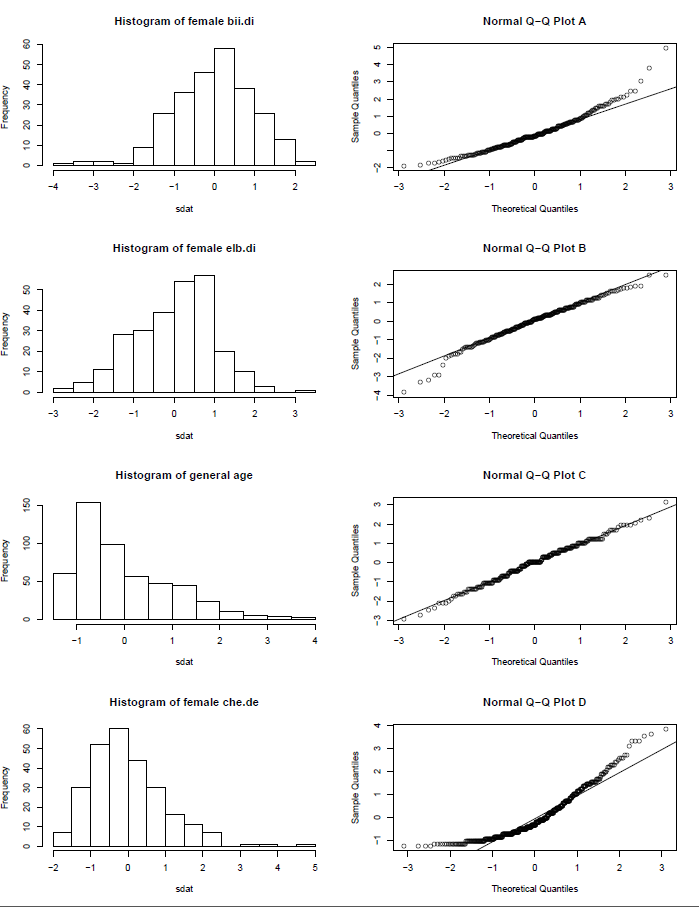
\includegraphics{./assets/images/04-01.png}
\caption{HistQMatch}
\end{figure}

\begin{itemize}
\item
  Note that normal probability plot D has a slight stepwise pattern. Why
  do you think this is the case?
\item
  As you can see, normal probability plots can be used both to assess
  normality and visualize skewness. Make a normal probability plot for
  female knee diameter (\texttt{kne.di}). Based on this normal
  probability plot, is this variable left skewed, symmetric, or right
  skewed? Use a histogram to confirm your findings.
\end{itemize}

\chapter{Foundations for Statistical Inference - Sampling
Distributions}\label{foundations-for-statistical-inference---sampling-distributions}

This lab is structured to guide you through an organized process such
that you could easily organize your code with comments --- meaning your
R script --- into a lab report. I would suggest getting into the habit
of writing an organized and commented R script that completes the tasks
and answers the questions provided in the lab --- including in the
\textbf{Own Your Own} section.

\begin{center}\rule{0.5\linewidth}{\linethickness}\end{center}

\section{Getting started}\label{getting-started-2}

In this lab, we investigate the ways in which the statistics from a
random sample of data can serve as point estimates for population
parameters. We're interested in formulating a \emph{sampling
distribution} of our estimate in order to learn about the properties of
the estimate, such as its distribution.

\section{The data}\label{the-data-1}

We consider real estate data from the city of Ames, Iowa. The details of
every real estate transaction in Ames is recorded by the City Assessor's
office. Our particular focus for this lab will be all residential home
sales in Ames between 2006 and 2010. This collection represents our
population of interest. In this lab we would like to learn about these
home sales by taking smaller samples from the full population. Let's
load the data.

\begin{Shaded}
\begin{Highlighting}[]
\KeywordTok{download.file}\NormalTok{(}\StringTok{"http://www.openintro.org/stat/data/ames.RData"}\NormalTok{, }\DataTypeTok{destfile =} \StringTok{"ames.RData"}\NormalTok{)}
\KeywordTok{load}\NormalTok{(}\StringTok{"ames.RData"}\NormalTok{)}
\end{Highlighting}
\end{Shaded}

We see that there are quite a few variables in the data set, enough to
do a very in-depth analysis. For this lab, we'll restrict our attention
to just two of the variables: the above ground living area of the house
in square feet (\texttt{Gr.Liv.Area}) and the sale price
(\texttt{SalePrice}). To save some effort throughout the lab, create two
variables with short names that represent these two variables.

\begin{Shaded}
\begin{Highlighting}[]
\NormalTok{area <-}\StringTok{ }\NormalTok{ames$Gr.Liv.Area}
\NormalTok{price <-}\StringTok{ }\NormalTok{ames$SalePrice}
\end{Highlighting}
\end{Shaded}

Let's look at the distribution of area in our population of home sales
by calculating a few summary statistics and making a histogram.

\begin{Shaded}
\begin{Highlighting}[]
\KeywordTok{summary}\NormalTok{(area)}
\KeywordTok{hist}\NormalTok{(area)}
\KeywordTok{boxplot}\NormalTok{(area,}\DataTypeTok{horizontal =} \OtherTok{TRUE}\NormalTok{)}
\end{Highlighting}
\end{Shaded}

\begin{center}\rule{0.5\linewidth}{\linethickness}\end{center}

\textbf{Exercise 1:} Describe this population distribution.

\begin{center}\rule{0.5\linewidth}{\linethickness}\end{center}

\section{The unknown sampling
distribution}\label{the-unknown-sampling-distribution}

In this lab we have access to the entire population, but this is rarely
the case in real life. Gathering information on an entire population is
often extremely costly or impossible. Because of this, we often take a
sample of the population and use that to understand the properties of
the population.

If we were interested in estimating the mean living area in Ames based
on a sample, we can use the following command to survey the population.

\begin{Shaded}
\begin{Highlighting}[]
\NormalTok{samp1 <-}\StringTok{ }\KeywordTok{sample}\NormalTok{(area, }\DecValTok{50}\NormalTok{)}
\end{Highlighting}
\end{Shaded}

This command collects a simple random sample of size 50 from the vector
\texttt{area}, which is assigned to \texttt{samp1}. This is like going
into the City Assessor's database and pulling up the files on 50 random
home sales.Working with these 50 files would be considerably simpler
than working with all 2930 home sales.

\begin{center}\rule{0.5\linewidth}{\linethickness}\end{center}

\textbf{Exercise 2:} Describe the distribution of this sample. How does
it compare to the distribution of the population?

\begin{center}\rule{0.5\linewidth}{\linethickness}\end{center}

If we're interested in estimating the average living area in homes in
Ames using the sample, our best single guess is the sample mean.

\begin{Shaded}
\begin{Highlighting}[]
\KeywordTok{mean}\NormalTok{(samp1)}
\end{Highlighting}
\end{Shaded}

Depending on which 50 homes you selected, your estimate could be a bit
above or a bit below the true population mean of 1499.69 square feet. In
general, though, the sample mean turns out to be a pretty good estimate
of the average living area, and we were able to get it by sampling less
than 3\% of the population.

\begin{center}\rule{0.5\linewidth}{\linethickness}\end{center}

\textbf{Exercise 3:} Take a second sample, also of size 50, and call it
\texttt{samp2}. How does the mean of \texttt{samp2} compare with the
mean of \texttt{samp1}? Suppose we took two more samples, one of size
100 and one of size 1000. Which would you think would provide a more
accurate estimate of the population mean?

\begin{center}\rule{0.5\linewidth}{\linethickness}\end{center}

Not surprisingly, every time we take another random sample, we get a
different sample mean. It's useful to get a sense of just how much
variability we should expect when estimating the population mean this
way. The distribution of sample means, called the \emph{sampling
distribution}, can help us understand this variability. In this lab,
because we have access to the population, we can build up the sampling
distribution for the sample mean by repeating the above steps many
times. Here we will generate 5000 samples and compute the sample mean of
each.

\begin{Shaded}
\begin{Highlighting}[]
\NormalTok{sample_means50 <-}\StringTok{ }\KeywordTok{rep}\NormalTok{(}\OtherTok{NA}\NormalTok{, }\DecValTok{5000}\NormalTok{)}

\NormalTok{for(i in }\DecValTok{1}\NormalTok{:}\DecValTok{5000}\NormalTok{)\{}
   \NormalTok{samp <-}\StringTok{ }\KeywordTok{sample}\NormalTok{(area, }\DecValTok{50}\NormalTok{)}
   \NormalTok{sample_means50[i] <-}\StringTok{ }\KeywordTok{mean}\NormalTok{(samp)}
   \NormalTok{\}}

\KeywordTok{hist}\NormalTok{(sample_means50)}
\end{Highlighting}
\end{Shaded}

If you would like to adjust the bin width of your histogram to show a
little more detail, you can do so by changing the \texttt{breaks}
argument.

\begin{Shaded}
\begin{Highlighting}[]
\KeywordTok{hist}\NormalTok{(sample_means50, }\DataTypeTok{breaks =} \DecValTok{25}\NormalTok{)}
\end{Highlighting}
\end{Shaded}

Here we use R to take 5000 samples of size 50 from the population,
calculate the mean of each sample, and store each result in a vector
called \texttt{sample\_means50}. On the next page, we'll review how this
set of code works.

\begin{center}\rule{0.5\linewidth}{\linethickness}\end{center}

\textbf{Exercise 4:} How many elements are there in
\texttt{sample\_means50}? Describe the sampling distribution, and be
sure to specifically note its center. Would you expect the distribution
to change if we instead collected 50,000 sample means?

\begin{center}\rule{0.5\linewidth}{\linethickness}\end{center}

\section{\texorpdfstring{Interlude: The \texttt{for}
loop}{Interlude: The for loop}}\label{interlude-the-for-loop}

Let's take a break from the statistics for a moment to let that last
block of code sink in. You have just run your first \texttt{for} loop, a
cornerstone of computer programming. The idea behind the for loop is
\emph{iteration}: it allows you to execute code as many times as you
want without having to type out every iteration. In the case above, we
wanted to iterate the two lines of code inside the curly braces that
take a random sample of size 50 from \texttt{area} then save the mean of
that sample into the \texttt{sample\_means50} vector. Without the
\texttt{for} loop, this would be painful:

\begin{Shaded}
\begin{Highlighting}[]
\NormalTok{sample_means50 <-}\StringTok{ }\KeywordTok{rep}\NormalTok{(}\OtherTok{NA}\NormalTok{, }\DecValTok{5000}\NormalTok{)}

\NormalTok{samp <-}\StringTok{ }\KeywordTok{sample}\NormalTok{(area, }\DecValTok{50}\NormalTok{)}
\NormalTok{sample_means50[}\DecValTok{1}\NormalTok{] <-}\StringTok{ }\KeywordTok{mean}\NormalTok{(samp)}

\NormalTok{samp <-}\StringTok{ }\KeywordTok{sample}\NormalTok{(area, }\DecValTok{50}\NormalTok{)}
\NormalTok{sample_means50[}\DecValTok{2}\NormalTok{] <-}\StringTok{ }\KeywordTok{mean}\NormalTok{(samp)}

\NormalTok{samp <-}\StringTok{ }\KeywordTok{sample}\NormalTok{(area, }\DecValTok{50}\NormalTok{)}
\NormalTok{sample_means50[}\DecValTok{3}\NormalTok{] <-}\StringTok{ }\KeywordTok{mean}\NormalTok{(samp)}

\NormalTok{samp <-}\StringTok{ }\KeywordTok{sample}\NormalTok{(area, }\DecValTok{50}\NormalTok{)}
\NormalTok{sample_means50[}\DecValTok{4}\NormalTok{] <-}\StringTok{ }\KeywordTok{mean}\NormalTok{(samp)}
\end{Highlighting}
\end{Shaded}

and so on\ldots{}

With the for loop, these thousands of lines of code are compressed into
a handful of lines. We've added one extra line to the code below, which
prints the variable \texttt{i} during each iteration of the \texttt{for}
loop. Run this code.

\begin{Shaded}
\begin{Highlighting}[]
\NormalTok{sample_means50 <-}\StringTok{ }\KeywordTok{rep}\NormalTok{(}\OtherTok{NA}\NormalTok{, }\DecValTok{5000}\NormalTok{)}

\NormalTok{for(i in }\DecValTok{1}\NormalTok{:}\DecValTok{5000}\NormalTok{)\{}
   \NormalTok{samp <-}\StringTok{ }\KeywordTok{sample}\NormalTok{(area, }\DecValTok{50}\NormalTok{)}
   \NormalTok{sample_means50[i] <-}\StringTok{ }\KeywordTok{mean}\NormalTok{(samp)}
   \KeywordTok{print}\NormalTok{(i)}
   \NormalTok{\}}
\end{Highlighting}
\end{Shaded}

Let's consider this code line by line to figure out what it does. In the
first line we \emph{initialized a vector}. In this case, we created a
vector of 5000 zeros called \texttt{sample\_means50}. This vector will
will store values generated within the \texttt{for} loop.

The second line calls the \texttt{for} loop itself. The syntax can be
loosely read as, ``for every element \texttt{i} from 1 to 5000, run the
following lines of code''. You can think of \texttt{i} as the counter
that keeps track of which loop you're on. Therefore, more precisely, the
loop will run once when \texttt{i\ =\ 1}, then once when
\texttt{i\ =\ 2}, and so on up to \texttt{i\ =\ 5000}.

The body of the \texttt{for} loop is the part inside the curly braces,
and this set of code is run for each value of \texttt{i}. Here, on every
loop, we take a random sample of size 50 from \texttt{area}, take its
mean, and store it as the \(i\)th element of \texttt{sample\_means50}.

In order to display that this is really happening, we asked R to print
\texttt{i} at each iteration. This line of code is optional and is only
used for displaying what's going on while the \texttt{for} loop is
running.

The \texttt{for} loop allows us to not just run the code 5000 times, but
to neatly package the results, element by element, into the empty vector
that we initialized at the outset.

\begin{center}\rule{0.5\linewidth}{\linethickness}\end{center}

\textbf{Exercise 5:} To make sure you understand what you've done in
this loop, try running a smaller version. Initialize a vector of 100
zeros called \texttt{sample\_means\_small}. Run a loop that takes a
sample of size 50 from \texttt{area} and stores the sample mean in
\texttt{sample\_means\_small}, but only iterate from 1 to 100. Print the
output to your screen (type \texttt{sample\_means\_small} into the
console and press enter). How many elements are there in this object
called \texttt{sample\_means\_small}? What does each element represent?

\begin{center}\rule{0.5\linewidth}{\linethickness}\end{center}

\section{Sample size and the sampling
distribution}\label{sample-size-and-the-sampling-distribution}

Mechanics aside, let's return to the reason we used a \texttt{for} loop:
to compute a sampling distribution, specifically, this one.

\begin{Shaded}
\begin{Highlighting}[]
\KeywordTok{hist}\NormalTok{(sample_means50)}
\end{Highlighting}
\end{Shaded}

\textbf{The sampling distribution that we computed tells us much about
estimating the average living area in homes in Ames. Because the sample
mean is an unbiased estimator, the sampling distribution is centered at
the true average living area of the the population, and the spread of
the sampling distribution indicates how much variability is induced by
sampling only 50 home sales.}

To get a sense of the effect that sample size has on our distribution,
let's build up two more sampling distributions: one based on a sample
size of 10 and another based on a sample size of 100.

\begin{Shaded}
\begin{Highlighting}[]
\NormalTok{sample_means10 <-}\StringTok{ }\KeywordTok{rep}\NormalTok{(}\OtherTok{NA}\NormalTok{, }\DecValTok{5000}\NormalTok{)}
\NormalTok{sample_means100 <-}\StringTok{ }\KeywordTok{rep}\NormalTok{(}\OtherTok{NA}\NormalTok{, }\DecValTok{5000}\NormalTok{)}

\NormalTok{for(i in }\DecValTok{1}\NormalTok{:}\DecValTok{5000}\NormalTok{)\{}
  \NormalTok{samp <-}\StringTok{ }\KeywordTok{sample}\NormalTok{(area, }\DecValTok{10}\NormalTok{)}
  \NormalTok{sample_means10[i] <-}\StringTok{ }\KeywordTok{mean}\NormalTok{(samp)}
  \NormalTok{samp <-}\StringTok{ }\KeywordTok{sample}\NormalTok{(area, }\DecValTok{100}\NormalTok{)}
  \NormalTok{sample_means100[i] <-}\StringTok{ }\KeywordTok{mean}\NormalTok{(samp)}
\NormalTok{\}}
\end{Highlighting}
\end{Shaded}

Here we're able to use a single \texttt{for} loop to build two
distributions by adding additional lines inside the curly braces. Don't
worry about the fact that \texttt{samp} is used for the name of two
different objects. In the second command of the \texttt{for} loop, the
mean of \texttt{samp} is saved to the relevant place in the vector
\texttt{sample\_means10}. With the mean saved, we're now free to
overwrite the object \texttt{samp} with a new sample, this time of size
100. In general, anytime you create an object using a name that is
already in use, the old object will get replaced with the new one.

To see the effect that different sample sizes have on the sampling
distribution, plot the three distributions on top of one another.

\begin{Shaded}
\begin{Highlighting}[]
\KeywordTok{par}\NormalTok{(}\DataTypeTok{mfrow =} \KeywordTok{c}\NormalTok{(}\DecValTok{3}\NormalTok{, }\DecValTok{1}\NormalTok{))}

\NormalTok{xlimits <-}\StringTok{ }\KeywordTok{range}\NormalTok{(sample_means10)}

\KeywordTok{hist}\NormalTok{(sample_means10, }\DataTypeTok{breaks =} \DecValTok{20}\NormalTok{, }\DataTypeTok{xlim =} \NormalTok{xlimits)}
\KeywordTok{hist}\NormalTok{(sample_means50, }\DataTypeTok{breaks =} \DecValTok{20}\NormalTok{, }\DataTypeTok{xlim =} \NormalTok{xlimits)}
\KeywordTok{hist}\NormalTok{(sample_means100, }\DataTypeTok{breaks =} \DecValTok{20}\NormalTok{, }\DataTypeTok{xlim =} \NormalTok{xlimits)}
\end{Highlighting}
\end{Shaded}

The first command specifies that you'd like to divide the plotting area
into 3 rows and 1 column of plots (to return to the default setting of
plotting one at a time, use \texttt{par(mfrow\ =\ c(1,\ 1))}). The
\texttt{breaks} argument specifies the number of bins used in
constructing the histogram. The \texttt{xlim} argument specifies the
range of the x-axis of the histogram, and by setting it equal to
\texttt{xlimits} for each histogram, we ensure that all three histograms
will be plotted with the same limits on the x-axis.

\begin{center}\rule{0.5\linewidth}{\linethickness}\end{center}

\textbf{Exercise 6:} When the sample size is larger, what happens to the
center? What about the spread?

\begin{center}\rule{0.5\linewidth}{\linethickness}\end{center}

\section{On your own}\label{on-your-own-3}

So far, we have only focused on estimating the mean living area in homes
in Ames. Now you'll try to estimate the mean home price.

\begin{itemize}
\item
  Take a random sample of size 50 from \texttt{price}. Using this
  sample, what is your best point estimate of the population mean?
\item
  Since you have access to the population, simulate the sampling
  distribution for \(\bar{x}_{price}\) by taking 5000 samples from the
  population of size 50 and computing 5000 sample means. Store these
  means in a vector called \texttt{sample\_means50}. Plot the data, then
  describe the shape of this sampling distribution. Based on this
  sampling distribution, what would you guess the mean home price of the
  population to be? Finally, calculate and report the population mean.
\item
  Change your sample size from 50 to 150, then compute the sampling
  distribution using the same method as above, and store these means in
  a new vector called \texttt{sample\_means150}. Describe the shape of
  this sampling distribution, and compare it to the sampling
  distribution for a sample size of 50. Based on this sampling
  distribution, what would you guess to be the mean sale price of homes
  in Ames?
\item
  Of the sampling distributions from 2 and 3, which has a smaller
  spread? If we're concerned with making estimates that are more often
  close to the true value, would we prefer a distribution with a large
  or small spread?
\end{itemize}

\chapter{Confidence Intervals - Foundations for Statistical
Inference}\label{confidence-intervals---foundations-for-statistical-inference}

This lab is structured to guide you through an organized process such
that you could easily organize your code with comments --- meaning your
R script --- into a lab report. I would suggest getting into the habit
of writing an organized and commented R script that completes the tasks
and answers the questions provided in the lab -- including in the
\textbf{Own Your Own} section.

\begin{center}\rule{0.5\linewidth}{\linethickness}\end{center}

\section{Sampling from Ames, Iowa}\label{sampling-from-ames-iowa}

If you have access to data on an entire population, say the size of
every house in Ames, Iowa, it's straight forward to answer questions
like, ``How big is the typical house in Ames?'' and ``How much variation
is there in sizes of houses?''. If you have access to only a sample of
the population, as is often the case, the task becomes more complicated.
What is your best guess for the typical size if you only know the sizes
of several dozen houses? This sort of situation requires that you use
your sample to make inference on what your population looks like.

\section{The data}\label{the-data-2}

In the previous lab, ``Sampling Distributions'', we looked at the
population data of houses from Ames, Iowa. Let's start by loading that
data set.

\begin{Shaded}
\begin{Highlighting}[]
\KeywordTok{download.file}\NormalTok{(}\StringTok{"http://www.openintro.org/stat/data/ames.RData"}\NormalTok{, }\DataTypeTok{destfile =} \StringTok{"ames.RData"}\NormalTok{)}
\KeywordTok{load}\NormalTok{(}\StringTok{"ames.RData"}\NormalTok{)}
\end{Highlighting}
\end{Shaded}

In this lab we'll start with a simple random sample of size 60 from the
population. Specifically, this is a simple random sample of size 60.
Note that the data set has information on many housing variables, but
for the first portion of the lab we'll focus on the size of the house,
represented by the variable \texttt{Gr.Liv.Area}.

\begin{Shaded}
\begin{Highlighting}[]
\NormalTok{population <-}\StringTok{ }\NormalTok{ames$Gr.Liv.Area}
\NormalTok{samp <-}\StringTok{ }\KeywordTok{sample}\NormalTok{(population, }\DecValTok{60}\NormalTok{)}
\end{Highlighting}
\end{Shaded}

\begin{center}\rule{0.5\linewidth}{\linethickness}\end{center}

\textbf{Exercise 1:} Describe the distribution of your sample. What
would you say is the ``typical'' size within your sample? Also state
precisely what you interpreted ``typical'' to mean.

\textbf{Exercise 2:} Would you expect another student's distribution to
be identical to yours? Would you expect it to be similar? Why or why
not?

\begin{center}\rule{0.5\linewidth}{\linethickness}\end{center}

\section{Confidence intervals}\label{confidence-intervals}

One of the most common ways to describe the typical or central value of
a distribution is to use the mean. In this case we can calculate the
mean of the sample using,

\begin{Shaded}
\begin{Highlighting}[]
\NormalTok{sample_mean <-}\StringTok{ }\KeywordTok{mean}\NormalTok{(samp)}
\end{Highlighting}
\end{Shaded}

Return for a moment to the question that first motivated this lab: based
on this sample, what can we infer about the population? Based only on
this single sample, the best estimate of the average living area of
houses sold in Ames would be the sample mean, usually denoted as
\(\bar{x}\) (here we're calling it \texttt{sample\_mean}). That serves
as a good \emph{point estimate} but it would be useful to also
communicate how uncertain we are of that estimate. This can be captured
by using a \emph{confidence interval}.

We can calculate a 95\% confidence interval for a sample mean by adding
and subtracting 1.96 standard errors to the point estimate (See Section
4.2.3 if you are unfamiliar with this formula). Note that the 1.96 is
the result of rounding and we could ues R to find a more precise value
which is provided in the code below.

\begin{Shaded}
\begin{Highlighting}[]
\KeywordTok{qnorm}\NormalTok{(}\FloatTok{0.975}\NormalTok{) }\CommentTok{# or}
\KeywordTok{qnorm}\NormalTok{(}\FloatTok{0.025}\NormalTok{) }\CommentTok{# which is the negative version}
\end{Highlighting}
\end{Shaded}

Note that if we take 0.975 - 0.025 we get 0.95. Each tail is set to have
area 0.025. Usually two decimal places of accuracy is suffcient when
determining the appropriate \(z^*\) value for a given confidence level.
Therefore we will continue using 1.96, but keep the function above in
mind when you desire to use a different confidence level or you need
more precision.

\begin{Shaded}
\begin{Highlighting}[]
\NormalTok{se <-}\StringTok{ }\KeywordTok{sd}\NormalTok{(samp) /}\StringTok{ }\KeywordTok{sqrt}\NormalTok{(}\DecValTok{60}\NormalTok{)}
\NormalTok{lower <-}\StringTok{ }\NormalTok{sample_mean -}\StringTok{ }\FloatTok{1.96} \NormalTok{*}\StringTok{ }\NormalTok{se}
\NormalTok{upper <-}\StringTok{ }\NormalTok{sample_mean +}\StringTok{ }\FloatTok{1.96} \NormalTok{*}\StringTok{ }\NormalTok{se}
\KeywordTok{c}\NormalTok{(lower, upper)}
\end{Highlighting}
\end{Shaded}

This is an important inference that we've just made: even though we
don't know what the full population looks like, we're 95\% confident
that the true average size of houses in Ames lies between the values
\emph{lower} and \emph{upper}. There are a few conditions that must be
met for this interval to be valid.

\begin{center}\rule{0.5\linewidth}{\linethickness}\end{center}

\textbf{Exercise 3:} For the confidence interval to be valid, the sample
mean must be normally distributed and have standard error
\(s / \sqrt{n}.\) What conditions must be met for this to be true?

\begin{center}\rule{0.5\linewidth}{\linethickness}\end{center}

\section{Confidence levels}\label{confidence-levels}

\begin{center}\rule{0.5\linewidth}{\linethickness}\end{center}

\textbf{Exercise 4:} What does ``95\% confidence'' mean?

\begin{center}\rule{0.5\linewidth}{\linethickness}\end{center}

In this case we have the luxury of knowing the true population mean
since we have data on the entire population. This value can be
calculated using the following command:

\begin{Shaded}
\begin{Highlighting}[]
\KeywordTok{mean}\NormalTok{(population)}
\end{Highlighting}
\end{Shaded}

\begin{center}\rule{0.5\linewidth}{\linethickness}\end{center}

\textbf{Exercise 5:}Does your confidence interval capture the true
average size of houses in Ames? If you are working on this lab in a
classroom, does your neighbor's interval capture this value?

\textbf{Exercise 6:} Each student in your class should have gotten a
slightly different confidence interval. What proportion of those
intervals would you expect to capture the true population mean? Why? If
you are working in this lab in a classroom, collect data on the
intervals created by other students in the class and calculate the
proportion of intervals that capture the true population mean.

\begin{center}\rule{0.5\linewidth}{\linethickness}\end{center}

Using R, we're going to recreate many samples to learn more about how
sample means and confidence intervals vary from one sample to another.
\emph{Loops} come in handy here (If you are unfamiliar with loops,
review the \textbf{Foundations for Statistical Inference (Lab 04)}).

Here is the rough outline:

\begin{itemize}
\tightlist
\item
  Obtain a random sample.
\item
  Calculate and store the sample's mean and standard deviation.
\item
  Repeat steps (1) and (2) 500 times.
\item
  Use these stored statistics to calculate many confidence intervals.
\end{itemize}

But before we do all of this, we need to first create empty vectors
where we can save the means and standard deviations that will be
calculated from each sample. And while we're at it, let's also store the
desired sample size as \texttt{n}.

\begin{Shaded}
\begin{Highlighting}[]
\NormalTok{samp_mean <-}\StringTok{ }\KeywordTok{rep}\NormalTok{(}\OtherTok{NA}\NormalTok{, }\DecValTok{500}\NormalTok{)}
\NormalTok{samp_sd <-}\StringTok{ }\KeywordTok{rep}\NormalTok{(}\OtherTok{NA}\NormalTok{, }\DecValTok{500}\NormalTok{)}
\NormalTok{n <-}\StringTok{ }\DecValTok{60}
\end{Highlighting}
\end{Shaded}

Now we're ready for the loop where we calculate the means and standard
deviations of 500 random samples.

\begin{Shaded}
\begin{Highlighting}[]
\NormalTok{for(i in }\DecValTok{1}\NormalTok{:}\DecValTok{500}\NormalTok{)\{}
  \NormalTok{samp <-}\StringTok{ }\KeywordTok{sample}\NormalTok{(population, n) }\CommentTok{# obtain a sample of size n = 60 from the population}
  \NormalTok{samp_mean[i] <-}\StringTok{ }\KeywordTok{mean}\NormalTok{(samp)    }\CommentTok{# save sample mean in ith element of samp_mean}
  \NormalTok{samp_sd[i] <-}\StringTok{ }\KeywordTok{sd}\NormalTok{(samp)        }\CommentTok{# save sample sd in ith element of samp_sd}
\NormalTok{\}}
\end{Highlighting}
\end{Shaded}

Lastly, we construct the confidence intervals.

\begin{Shaded}
\begin{Highlighting}[]
\NormalTok{lower_vector <-}\StringTok{ }\NormalTok{samp_mean -}\StringTok{ }\FloatTok{1.96} \NormalTok{*}\StringTok{ }\NormalTok{samp_sd /}\StringTok{ }\KeywordTok{sqrt}\NormalTok{(n)}
\NormalTok{upper_vector <-}\StringTok{ }\NormalTok{samp_mean +}\StringTok{ }\FloatTok{1.96} \NormalTok{*}\StringTok{ }\NormalTok{samp_sd /}\StringTok{ }\KeywordTok{sqrt}\NormalTok{(n)}
\end{Highlighting}
\end{Shaded}

Lower bounds of these 500 confidence intervals are stored in
\texttt{lower\_vector}, and the upper bounds are in
\texttt{upper\_vector}. Let's view the first interval.

\begin{Shaded}
\begin{Highlighting}[]
\KeywordTok{c}\NormalTok{(lower_vector[}\DecValTok{1}\NormalTok{], upper_vector[}\DecValTok{1}\NormalTok{])}
\end{Highlighting}
\end{Shaded}

\begin{center}\rule{0.5\linewidth}{\linethickness}\end{center}

\section{On your own}\label{on-your-own-4}

\begin{itemize}
\item
  Using the function \texttt{plot\_ci()} (which was downloaded with the
  data set), we are able to plot the first fifity 95\% confidence
  intervals of our 500. What proportion of the 50 plotted confidence
  intervals include the true population mean? Is this proportion exactly
  equal to the confidence level? If not, explain why. Devise and
  implement a process to calculate the number (and proportion) of
  confidence intervals that include the true population for all 500 95\%
  confidence intervals - you don't want to have to plot and count by
  hand.

\begin{Shaded}
\begin{Highlighting}[]
\KeywordTok{plot_ci}\NormalTok{(lower_vector, upper_vector, }\KeywordTok{mean}\NormalTok{(population))}
\end{Highlighting}
\end{Shaded}
\item
  Suppose we want 90\% confidence intervals instead of 95\% confidence
  intervals. What is the appropriate critical value?
\item
  Construct 500 90\% confidence intervals. You do not need to obtain new
  samples, simply calculate new intervals based on the sample means and
  standard deviations you have already collected. Using the
  \texttt{plot\_ci} function, plot the first 50 90\% confidence
  intervals and calculate the proportion of intervals that include the
  true population mean. How does this percentage compare to the
  confidence level selected for the intervals? Using the method which
  you implemented in question 1 of the \textbf{On Your Own} section,
  determine the number (and proportion) of the 500 randomly generated
  90\% confidence intervals that include the true population mean.
\end{itemize}

\chapter{Inference for Numerical
Data}\label{inference-for-numerical-data}

\begin{center}\rule{0.5\linewidth}{\linethickness}\end{center}

The lab is structured to guide you through an organized process such
that you could easily organize your code with comments -- meaning your R
script -- into a lab report. I would suggest getting into the habit of
writing an organized and commented R script that completes the tasks and
answers the questions provided in the lab -- including in the
\textbf{Own Your Own} section.

\begin{center}\rule{0.5\linewidth}{\linethickness}\end{center}

\section{Overview}\label{overview}

We will be conducting hypothesis tests (HTs) and constructing confidence
intervals (CIs) for means and difference of means throughout this lab.
We will calculate them by ``hand'' and through the use of a built in
function in R called \texttt{t.test()}, which is an extremely useful and
flexible function when given the raw sample. Sometimes we are only given
access to sample statistics (e.g. \(\bar{x}\), \(s_x\), \(n\)), which
necessitates that we perform calculations by ``hand'' -- the function
\texttt{t.test()} requires the raw data.

\section{North Carolina births}\label{north-carolina-births}

In 2004, the state of North Carolina released a large data set
containing information on all births recorded in their state. This data
set is useful to researchers studying the relation between habits and
practices of expectant mothers and the birth of their children. We will
work with a random sample of observations from this data set.

\section{Exploratory analysis}\label{exploratory-analysis}

Load the \texttt{nc} data set into our workspace.

\begin{Shaded}
\begin{Highlighting}[]
\KeywordTok{download.file}\NormalTok{(}\StringTok{"http://www.openintro.org/stat/data/nc.RData"}\NormalTok{, }\DataTypeTok{destfile =} \StringTok{"nc.RData"}\NormalTok{)}
\KeywordTok{load}\NormalTok{(}\StringTok{"nc.RData"}\NormalTok{)}
\end{Highlighting}
\end{Shaded}

We observations of 13 different variables, some categorical and some
numerical. The meaning of each variable is as follows:

\begin{longtable}[]{@{}ll@{}}
\toprule
\begin{minipage}[b]{0.22\columnwidth}\raggedright\strut
variable\strut
\end{minipage} & \begin{minipage}[b]{0.16\columnwidth}\raggedright\strut
description\strut
\end{minipage}\tabularnewline
\midrule
\endhead
\begin{minipage}[t]{0.22\columnwidth}\raggedright\strut
\texttt{fage}\strut
\end{minipage} & \begin{minipage}[t]{0.16\columnwidth}\raggedright\strut
father's age in years.\strut
\end{minipage}\tabularnewline
\begin{minipage}[t]{0.22\columnwidth}\raggedright\strut
\texttt{mage}\strut
\end{minipage} & \begin{minipage}[t]{0.16\columnwidth}\raggedright\strut
mother's age in years.\strut
\end{minipage}\tabularnewline
\begin{minipage}[t]{0.22\columnwidth}\raggedright\strut
\texttt{mature}\strut
\end{minipage} & \begin{minipage}[t]{0.16\columnwidth}\raggedright\strut
maturity status of mother.\strut
\end{minipage}\tabularnewline
\begin{minipage}[t]{0.22\columnwidth}\raggedright\strut
\texttt{weeks}\strut
\end{minipage} & \begin{minipage}[t]{0.16\columnwidth}\raggedright\strut
length of pregnancy in weeks.\strut
\end{minipage}\tabularnewline
\begin{minipage}[t]{0.22\columnwidth}\raggedright\strut
\texttt{premie}\strut
\end{minipage} & \begin{minipage}[t]{0.16\columnwidth}\raggedright\strut
whether the birth was classified as premature (premie) or
full-term.\strut
\end{minipage}\tabularnewline
\begin{minipage}[t]{0.22\columnwidth}\raggedright\strut
\texttt{visits}\strut
\end{minipage} & \begin{minipage}[t]{0.16\columnwidth}\raggedright\strut
number of hospital visits during pregnancy.\strut
\end{minipage}\tabularnewline
\begin{minipage}[t]{0.22\columnwidth}\raggedright\strut
\texttt{marital}\strut
\end{minipage} & \begin{minipage}[t]{0.16\columnwidth}\raggedright\strut
whether mother is \texttt{married} or \texttt{not\ married} at
birth.\strut
\end{minipage}\tabularnewline
\begin{minipage}[t]{0.22\columnwidth}\raggedright\strut
\texttt{gained}\strut
\end{minipage} & \begin{minipage}[t]{0.16\columnwidth}\raggedright\strut
weight gained by mother during pregnancy in pounds.\strut
\end{minipage}\tabularnewline
\begin{minipage}[t]{0.22\columnwidth}\raggedright\strut
\texttt{weight}\strut
\end{minipage} & \begin{minipage}[t]{0.16\columnwidth}\raggedright\strut
weight of the baby at birth in pounds.\strut
\end{minipage}\tabularnewline
\begin{minipage}[t]{0.22\columnwidth}\raggedright\strut
\texttt{lowbirthweight}\strut
\end{minipage} & \begin{minipage}[t]{0.16\columnwidth}\raggedright\strut
whether baby was classified as low birthweight (\texttt{low}) or not
(\texttt{not\ low}).\strut
\end{minipage}\tabularnewline
\begin{minipage}[t]{0.22\columnwidth}\raggedright\strut
\texttt{gender}\strut
\end{minipage} & \begin{minipage}[t]{0.16\columnwidth}\raggedright\strut
gender of the baby, \texttt{female} or \texttt{male}.\strut
\end{minipage}\tabularnewline
\begin{minipage}[t]{0.22\columnwidth}\raggedright\strut
\texttt{habit}\strut
\end{minipage} & \begin{minipage}[t]{0.16\columnwidth}\raggedright\strut
status of the mother as a \texttt{nonsmoker} or a \texttt{smoker}.\strut
\end{minipage}\tabularnewline
\begin{minipage}[t]{0.22\columnwidth}\raggedright\strut
\texttt{whitemom}\strut
\end{minipage} & \begin{minipage}[t]{0.16\columnwidth}\raggedright\strut
whether mom is \texttt{white} or \texttt{not\ white}.\strut
\end{minipage}\tabularnewline
\bottomrule
\end{longtable}

\begin{quote}
\textbf{Exercise 1:} What are the cases in this data set? How many cases
are there in our sample?
\end{quote}

As a first step in the analysis, we should consider summaries of the
data. This can be done using the \texttt{summary} command:

\begin{Shaded}
\begin{Highlighting}[]
\KeywordTok{summary}\NormalTok{(nc)}
\end{Highlighting}
\end{Shaded}

As you review the variable summaries, consider which variables are
categorical and which are numerical. For numerical variables, are there
outliers? If you aren't sure or want to take a closer look at the data,
make a graph.

Suppose we want to investigate the typical age for mothers and fathers
in North Carolina. Begin by constructing histograms, box plots, and
calculating summary statistics.

\begin{Shaded}
\begin{Highlighting}[]
\CommentTok{# Mother's age}
\KeywordTok{hist}\NormalTok{(nc$mage)}
\KeywordTok{boxplot}\NormalTok{(nc$mage, }\DataTypeTok{horizontal =} \OtherTok{TRUE}\NormalTok{)}
\KeywordTok{summary}\NormalTok{(nc$mage)}
\KeywordTok{sd}\NormalTok{(nc$mage)}
\KeywordTok{IQR}\NormalTok{(nc$mage)}

\CommentTok{# Father's age}
\KeywordTok{hist}\NormalTok{(nc$fage)}
\KeywordTok{boxplot}\NormalTok{(nc$fage, }\DataTypeTok{horizontal =} \OtherTok{TRUE}\NormalTok{)}
\KeywordTok{summary}\NormalTok{(nc$fage)}
\KeywordTok{sd}\NormalTok{(nc$fage)}
\KeywordTok{IQR}\NormalTok{(nc$fage)}
\end{Highlighting}
\end{Shaded}

Note that \texttt{sd(nc\$fage)} or \texttt{IQR(nc\$fage)} do not return
valid output/values. The summary output indicated that there were 171
births where a father's age was missing or not reported. By default most
R function will not return valid output when data is missing. This can
be fixed by adding the argument \texttt{na.rm\ =\ TRUE} in the function
call -- see below.

\begin{Shaded}
\begin{Highlighting}[]
\CommentTok{# Father's age continued}
\KeywordTok{sd}\NormalTok{(nc$fage, }\DataTypeTok{na.rm =} \OtherTok{TRUE}\NormalTok{)}
\KeywordTok{IQR}\NormalTok{(nc$fage, }\DataTypeTok{na.rm =} \OtherTok{TRUE}\NormalTok{)}
\end{Highlighting}
\end{Shaded}

Suppose we want to test the hypothesis that the mean age for women
giving birth in North Carolina is 26.5 years. Calculating by ``hand'':

\begin{Shaded}
\begin{Highlighting}[]
\CommentTok{# Sample Data}
\NormalTok{xbar <-}\StringTok{ }\KeywordTok{mean}\NormalTok{(nc$mage)}
\NormalTok{std <-}\StringTok{ }\KeywordTok{sd}\NormalTok{(nc$mage)}
\NormalTok{samp_size <-}\StringTok{ }\KeywordTok{length}\NormalTok{(nc$mage)}

\CommentTok{# Hypothesis Test -- Calculating p-value}
\NormalTok{dof <-}\StringTok{ }\NormalTok{samp_size -}\StringTok{ }\DecValTok{1}
\NormalTok{std_err <-}\StringTok{ }\NormalTok{std/}\KeywordTok{sqrt}\NormalTok{(samp_size)}
\NormalTok{test_stat <-}\StringTok{ }\NormalTok{(xbar -}\StringTok{ }\FloatTok{26.5}\NormalTok{)/std_err}
\NormalTok{p_value <-}\StringTok{ }\DecValTok{2}\NormalTok{*}\KeywordTok{pt}\NormalTok{(-}\KeywordTok{abs}\NormalTok{(test_stat),}\DataTypeTok{df =} \NormalTok{dof)}
\NormalTok{p_value}

\CommentTok{# Constructing 95% CI for the mean}
\NormalTok{t_star <-}\StringTok{ }\KeywordTok{qt}\NormalTok{(}\DataTypeTok{p =} \NormalTok{.}\DecValTok{975}\NormalTok{, }\DataTypeTok{df =} \NormalTok{dof)}
\NormalTok{LB <-}\StringTok{ }\NormalTok{xbar -}\StringTok{ }\NormalTok{t_star*std_err}
\NormalTok{UB <-}\StringTok{ }\NormalTok{xbar +}\StringTok{ }\NormalTok{t_star*std_err}
\KeywordTok{c}\NormalTok{(LB,UB)}
\end{Highlighting}
\end{Shaded}

Since our p-value is less than significance level \(\alpha\) (0.05), we
have sufficient evidence to reject that the mean age of women giving
birth in North Carolina is 26.5 years old. Note that 26.5 is not in the
95\% confidence interval for the mean age of birthing women in NC.
Two-tailed hypothesis tests for the mean with significance level
\(\alpha\) are logically equivalent to \(100(1-\alpha)\%\) confidence
interval for the mean -- \textbf{this is a big deal}.

Let's make use of the \texttt{t.test()} function now. The function has
several inputs that you should become familiar with and work to
understand.

\begin{Shaded}
\begin{Highlighting}[]
\CommentTok{# Mother's mean age -- HT and 95% CI}
\KeywordTok{t.test}\NormalTok{(}\DataTypeTok{x =} \NormalTok{nc$mage, }\DataTypeTok{alternative =} \StringTok{"two.sided"}\NormalTok{, }\DataTypeTok{mu =} \FloatTok{26.5}\NormalTok{, }\DataTypeTok{conf.level =} \FloatTok{0.95}\NormalTok{)}
\end{Highlighting}
\end{Shaded}

\begin{quote}
\textbf{Exercise 2:} Suppose now we want test whether the mean age of NC
fathers is 30 years. Use \(\alpha = 0.01\). Also construct a 99\%
confidence interval for the mean. Calculate by ``hand'' and by using
\texttt{t.test()}. \emph{Hint: When calculating by ``hand'', missing
values can be an issue so first extract and store the useful
observations as shown below. The \texttt{t.test()} takes care of
missingness automatically.}
\end{quote}

\begin{Shaded}
\begin{Highlighting}[]
\CommentTok{# Extract and store useful data}
\NormalTok{keep_condition <-}\StringTok{ }\NormalTok{!}\KeywordTok{is.na}\NormalTok{(nc$fage)}
\NormalTok{f_age <-}\StringTok{ }\NormalTok{nc$fage[keep_condition]}
\end{Highlighting}
\end{Shaded}

Suppose a researcher wants to test the hypothesis that in NC the mean
age of fathers is different than the mean age of mothers at birth --
assume an \(\alpha = 0.01\). This is a test for the difference in two
population means, which requires us to ask whether the data for the two
groups (mothers and fathers) is paired or not. Clearly, the data is
paired since each mother and father can be reasonably matched together.
First by ``hand'',

\begin{Shaded}
\begin{Highlighting}[]
\CommentTok{# Paired -- only need the differences in age}
\NormalTok{age_diff <-}\StringTok{ }\NormalTok{nc$mage -}\StringTok{ }\NormalTok{nc$fage  }
\KeywordTok{summary}\NormalTok{(age_diff)}

\CommentTok{# Diff. sample statistics -- note their are missing values}
\NormalTok{xbar <-}\StringTok{ }\KeywordTok{mean}\NormalTok{(age_diff, }\DataTypeTok{na.rm =} \OtherTok{TRUE}\NormalTok{)}
\NormalTok{std <-}\StringTok{ }\KeywordTok{sd}\NormalTok{(age_diff, }\DataTypeTok{na.rm =} \OtherTok{TRUE}\NormalTok{)}
\NormalTok{samp_size <-}\StringTok{ }\KeywordTok{sum}\NormalTok{(!}\KeywordTok{is.na}\NormalTok{(age_diff))}

\CommentTok{# Hypothesis Test -- Calculating p-value}
\NormalTok{dof <-}\StringTok{ }\NormalTok{samp_size -}\StringTok{ }\DecValTok{1}
\NormalTok{std_err <-}\StringTok{ }\NormalTok{std/}\KeywordTok{sqrt}\NormalTok{(samp_size)}
\NormalTok{test_stat <-}\StringTok{ }\NormalTok{(xbar -}\StringTok{ }\DecValTok{0}\NormalTok{)/std_err}
\NormalTok{p_value <-}\StringTok{ }\DecValTok{2}\NormalTok{*}\KeywordTok{pt}\NormalTok{(-}\KeywordTok{abs}\NormalTok{(test_stat),}\DataTypeTok{df =} \NormalTok{dof)}
\NormalTok{p_value}

\CommentTok{# Constructing 99% CI for the mean}
\NormalTok{t_star <-}\StringTok{ }\KeywordTok{qt}\NormalTok{(}\DataTypeTok{p =} \NormalTok{.}\DecValTok{995}\NormalTok{, }\DataTypeTok{df =} \NormalTok{dof)}
\NormalTok{LB <-}\StringTok{ }\NormalTok{xbar -}\StringTok{ }\NormalTok{t_star*std_err}
\NormalTok{UB <-}\StringTok{ }\NormalTok{xbar +}\StringTok{ }\NormalTok{t_star*std_err}
\KeywordTok{c}\NormalTok{(LB,UB)}
\end{Highlighting}
\end{Shaded}

Using \texttt{t.test()} -- a few coding options.

\begin{Shaded}
\begin{Highlighting}[]
\CommentTok{# Option 1: Calculate the differences externally and feed}
\CommentTok{# them into the t.test function}
\KeywordTok{t.test}\NormalTok{(}\DataTypeTok{x =} \NormalTok{age_diff, }\DataTypeTok{alternative =} \StringTok{"two.sided"}\NormalTok{, }\DataTypeTok{mu =} \DecValTok{0}\NormalTok{, }\DataTypeTok{conf.level =} \FloatTok{0.99}\NormalTok{)}

\CommentTok{# Option 2: Let the function calculate the differences by}
\CommentTok{# setting paired = TRUE}
\KeywordTok{t.test}\NormalTok{(}\DataTypeTok{x =} \NormalTok{nc$mage, }\DataTypeTok{y =} \NormalTok{nc$fage, }\DataTypeTok{alternative =} \StringTok{"two.sided"}\NormalTok{, }\DataTypeTok{mu =} \DecValTok{0}\NormalTok{, }\DataTypeTok{paired =} \OtherTok{TRUE}\NormalTok{)}
\end{Highlighting}
\end{Shaded}

Now consider the possible relationship between a mother's smoking habit
and the weight of her baby. Plotting the data is a useful first step
because it helps us quickly visualize trends, identify strong
associations, and develop research questions.

\begin{quote}
\textbf{Exercise 3:} Make a side-by-side box plot of \texttt{habit} and
\texttt{weight}. What does the plot highlight about the relationship
between these two variables?
\end{quote}

The box plots show how the medians of the two distributions compare, but
we can also compare the means of the distributions using the following
function to split the \texttt{weight} variable into the \texttt{habit}
groups, then take the mean of each using the \texttt{mean} function.

\begin{Shaded}
\begin{Highlighting}[]
\KeywordTok{by}\NormalTok{(nc$weight, nc$habit, mean)}
\end{Highlighting}
\end{Shaded}

There is an observed difference, but is this difference statistically
significant? In order to answer this question we will conduct a
hypothesis test.

\begin{quote}
\textbf{Exercise 4:} Check if the conditions necessary for inference are
satisfied. Note that you will need to obtain sample sizes to check the
conditions. You can compute the group size using the same \texttt{by}
command above but replacing \texttt{mean} with \texttt{length}.
\end{quote}

\begin{quote}
\textbf{Exercise 5:} Write the hypotheses for testing if the average
weights of babies born to smoking and non-smoking mothers are different.
\end{quote}

Again, this a hypothesis test for a difference of two means, but in this
case the data is not paired -- there is no reasonable way of matching
members from one group (smokers) to the other (non-smokers). Are the two
groups independent from one another? There is no reason to believe that
the groups are dependent since the records were randomly sampled. First
by ``hand'',

\begin{Shaded}
\begin{Highlighting}[]
\CommentTok{# Sample statistics for baby weights for smoking mothers}
\NormalTok{grp1 <-}\StringTok{ }\NormalTok{nc$weight[nc$habit ==}\StringTok{ "smoker"}\NormalTok{]}
\NormalTok{xbar1 <-}\StringTok{ }\KeywordTok{mean}\NormalTok{(grp1, }\DataTypeTok{na.rm =} \OtherTok{TRUE}\NormalTok{)}
\NormalTok{std1 <-}\StringTok{ }\KeywordTok{sd}\NormalTok{(grp1, }\DataTypeTok{na.rm =} \OtherTok{TRUE}\NormalTok{)}
\NormalTok{samp_size1 <-}\StringTok{ }\KeywordTok{sum}\NormalTok{(!}\KeywordTok{is.na}\NormalTok{(grp1))}

\CommentTok{# Sample statistics for baby weights for nonsmoking mothers}
\NormalTok{grp2 <-}\StringTok{ }\NormalTok{nc$weight[nc$habit ==}\StringTok{ "nonsmoker"}\NormalTok{]}
\NormalTok{xbar2 <-}\StringTok{ }\KeywordTok{mean}\NormalTok{(grp2, }\DataTypeTok{na.rm =} \OtherTok{TRUE}\NormalTok{)}
\NormalTok{std2 <-}\StringTok{ }\KeywordTok{sd}\NormalTok{(grp2, }\DataTypeTok{na.rm =} \OtherTok{TRUE}\NormalTok{)}
\NormalTok{samp_size2 <-}\StringTok{ }\KeywordTok{sum}\NormalTok{(!}\KeywordTok{is.na}\NormalTok{(grp2))}

\CommentTok{# Hypothesis Test -- Calculating p-value}
\NormalTok{dof <-}\StringTok{ }\KeywordTok{min}\NormalTok{(}\KeywordTok{c}\NormalTok{(samp_size1,samp_size2)) -}\StringTok{ }\DecValTok{1} 
\NormalTok{std_err <-}\StringTok{ }\KeywordTok{sqrt}\NormalTok{(std1^}\DecValTok{2}\NormalTok{/samp_size1 +}\StringTok{ }\NormalTok{std2^}\DecValTok{2}\NormalTok{/samp_size2)}
\NormalTok{test_stat <-}\StringTok{ }\NormalTok{(xbar1-xbar2 -}\StringTok{ }\DecValTok{0}\NormalTok{)/std_err}
\NormalTok{p_value <-}\StringTok{ }\DecValTok{2}\NormalTok{*}\KeywordTok{pt}\NormalTok{(-}\KeywordTok{abs}\NormalTok{(test_stat),}\DataTypeTok{df =} \NormalTok{dof)}
\NormalTok{p_value}

\CommentTok{# Constructing 95% CI for the mean}
\NormalTok{t_star <-}\StringTok{ }\KeywordTok{qt}\NormalTok{(}\DataTypeTok{p =} \NormalTok{.}\DecValTok{975}\NormalTok{, }\DataTypeTok{df =} \NormalTok{dof)}
\NormalTok{LB <-}\StringTok{ }\NormalTok{(xbar1 -}\StringTok{ }\NormalTok{xbar2) -}\StringTok{ }\NormalTok{t_star*std_err}
\NormalTok{UB <-}\StringTok{ }\NormalTok{(xbar1 -}\StringTok{ }\NormalTok{xbar2) +}\StringTok{ }\NormalTok{t_star*std_err}
\KeywordTok{c}\NormalTok{(LB,UB)}
\end{Highlighting}
\end{Shaded}

Using \texttt{t.test()}.

\begin{Shaded}
\begin{Highlighting}[]
\CommentTok{# Note taht grp1 and grp2 come from above}
\KeywordTok{t.test}\NormalTok{(}\DataTypeTok{x =} \NormalTok{grp1, }\DataTypeTok{y =} \NormalTok{grp2, }\DataTypeTok{alternative =} \StringTok{"two.sided"}\NormalTok{, }\DataTypeTok{mu =} \DecValTok{0}\NormalTok{, }\DataTypeTok{var.equal =} \OtherTok{FALSE}\NormalTok{, }\DataTypeTok{conf.level =} \NormalTok{.}\DecValTok{95}\NormalTok{)}
\end{Highlighting}
\end{Shaded}

\textbf{Notice that the by ``hand'' calculations and the results from
\texttt{t.test()} do not match.} The difference is caused by the use of
different degrees of freedom calculations. The software is utilizing the
exact calculation for the degrees of freedom while we are utilizing a
\emph{conservative} estimate to the degrees of freedom.

Also note \texttt{var.equal\ =} is an indicator/flag for whether we are
willing to make the assumption that the two groups have equal variance
(i.e.~spread/variability). In most cases it is safer not to make this
assumption, thus the default is \texttt{FALSE}. Although, some software
and researchers will make this assumption. Set
\texttt{var.equal\ =\ TRUE} and see what happens. \textbf{What affect
did this assumption have on the p-value and confidence interval?}

\begin{center}\rule{0.5\linewidth}{\linethickness}\end{center}

\section{On your own}\label{on-your-own-5}

\begin{itemize}
\item
  Calculate a 95\% confidence interval for the average length of
  pregnancies (\texttt{weeks}) and interpret it in context.
\item
  Calculate a new confidence interval for the same parameter at the 90\%
  confidence level.
\item
  Conduct a hypothesis test evaluating whether the average weight gained
  by younger mothers is different than the average weight gained by
  mature mothers.
\item
  Now, a non-inference task: Determine the age cutoff for younger and
  mature mothers. Use a method of your choice, and explain how your
  method works.
\item
  Pick a pair of numerical and categorical variables and come up with a
  research question evaluating the relationship between these variables.
  Formulate the question in a way that it can be answered using a
  hypothesis test and/or a confidence interval. Answer your question
  using the \texttt{t.test()} function, report the statistical results,
  and also provide an explanation in plain language.
\end{itemize}

\chapter{Inference for Categorical
Data}\label{inference-for-categorical-data}

This lab is structured to guide you through an organized process such
that you could easily organize your code with comments --- meaning your
R script --- into a lab report. I would suggest getting into the habit
of writing an organized and commented R script that completes the tasks
and answers the questions provided in the lab --- including in the
\textbf{Own Your Own} section.

\begin{center}\rule{0.5\linewidth}{\linethickness}\end{center}

\subsection{Getting Started}\label{getting-started-3}

In August of 2012, news outlets ranging from the
\href{http://www.washingtonpost.com/national/on-faith/poll-shows-atheism-on-the-rise-in-the-us/2012/08/13/90020fd6-e57d-11e1-9739-eef99c5fb285_story.html}{Washington
Post} to the
\href{http://www.huffingtonpost.com/2012/08/14/atheism-rise-religiosity-decline-in-america_n_1777031.html}{Huffington
Post} ran a story about the rise of atheism in America. The source for
the story was a poll that asked people, ``Irrespective of whether you
attend a place of worship or not, would you say you are a religious
person, not a religious person or a convinced atheist?'' This type of
question, which asks people to classify themselves in one way or
another, is common in polling and generates categorical data. In this
lab we take a look at the atheism survey and explore what's at play when
making inference about population proportions using categorical data.

\section{The survey}\label{the-survey}

To download a copy of the press release for the poll, conducted by
WIN-Gallup International, click on the following link:

\href{https://github.com/nulib/kuyper-stat202/raw/master/assets/support_doc/Global_INDEX_of_Religiosity_and_Atheism_PR_6.pdf}{Download
the Press Release}

Take a moment to review the report, then address the following
questions.

\begin{center}\rule{0.5\linewidth}{\linethickness}\end{center}

\textbf{Exercise 1:} In the first paragraph, several key findings are
reported. Do these percentages appear to be \emph{sample statistics}
(derived from the sample data) or \emph{population parameters}?

\textbf{Exercise 2:} The title of the report is ``Global Index of
Religiosity and Atheism''. To generalize the report's findings to the
global human population, what must we assume about the sampling method?
Does that seem like a reasonable assumption?

\begin{center}\rule{0.5\linewidth}{\linethickness}\end{center}

\section{The data}\label{the-data-3}

Turn your attention to Table 6 (pages 15 and 16), which reports the
sample size and response percentages for all 57 countries. While this is
a useful format to summarize the data, we will base our analysis on the
original data set of individual responses to the survey. Load this
dataset into R with the following command.

\begin{Shaded}
\begin{Highlighting}[]
\KeywordTok{download.file}\NormalTok{(}\StringTok{"http://www.openintro.org/stat/data/atheism.RData"}\NormalTok{, }\DataTypeTok{destfile =} \StringTok{"atheism.RData"}\NormalTok{)}
\KeywordTok{load}\NormalTok{(}\StringTok{"atheism.RData"}\NormalTok{)}
\end{Highlighting}
\end{Shaded}

\begin{center}\rule{0.5\linewidth}{\linethickness}\end{center}

\textbf{Exercise 3:} What does each row of Table 6 correspond to? What
does each row of \texttt{atheism} correspond to?

\begin{center}\rule{0.5\linewidth}{\linethickness}\end{center}

To investigate the link between these two ways of organizing this data,
take a look at the estimated proportion of atheists in the United
States. Towards the bottom of Table 6, we see that this is 5\%. We
should be able to come to the same number using the \texttt{atheism}
data.

\begin{center}\rule{0.5\linewidth}{\linethickness}\end{center}

\textbf{Exercise 4:} Using the command below, create a new dataframe
called \texttt{us12} that contains only the rows in \texttt{atheism}
associated with respondents to the 2012 survey from the United States.
Next, calculate the proportion of atheist responses. Does it agree with
the percentage in Table 6? If not, why?

\begin{center}\rule{0.5\linewidth}{\linethickness}\end{center}

\begin{Shaded}
\begin{Highlighting}[]
\NormalTok{us12 <-}\StringTok{ }\KeywordTok{subset}\NormalTok{(atheism, nationality ==}\StringTok{ "United States"} \NormalTok{&}\StringTok{ }\NormalTok{year ==}\StringTok{ "2012"}\NormalTok{)}
\end{Highlighting}
\end{Shaded}

\section{Inference on proportions}\label{inference-on-proportions}

As was hinted at in Exercise 1, Table 6 provides \emph{statistics}, that
is, calculations made from the sample of 51,927 people. What we'd like,
though, is insight into the population \emph{parameters}. You answer the
question, ``What proportion of people in your sample reported being
atheists?'' with a statistic; while the question ``What proportion of
people on earth would report being atheists'' is answered with an
estimate of the parameter.

The inferential tools for estimating population proportion are analogous
to those used for means in the last chapter: the confidence interval and
the hypothesis test.

\begin{quote}
\textbf{Exercise 5:} Write out the conditions for inference to construct
a 95\% confidence interval for the proportion of atheists in the United
States in 2012. Are you confident all conditions are met?
\end{quote}

If the conditions for inference are reasonable, we can calculate the
standard error and construct the interval by ``hand'' as outlined in our
book. Note that since the goal is to construct an interval estimate for
a proportion, it's necessary to specify what constitutes a ``success'',
which here is a response of \texttt{"atheist"}.

\begin{Shaded}
\begin{Highlighting}[]
\CommentTok{# First we need to identify the successes and failures}
\CommentTok{# We can find out what our options with the following}
\KeywordTok{levels}\NormalTok{(us12$response)}

\CommentTok{# Since we are looking for atheist we define a success as}
\CommentTok{# "atheist" and a failure as not atheist (regarless of other}
\CommentTok{# categories)}
\CommentTok{# -- code returns TRUE for atheist and FALSE otherwise}
\NormalTok{atheist_yes_no <-}\StringTok{ }\NormalTok{us12$response ==}\StringTok{ "atheist"}

\CommentTok{# Checking how many atheist and non-atheist are in the sample}
\CommentTok{# Also a check to verify we have at least 10 successes and failures}
\KeywordTok{table}\NormalTok{(atheist_yes_no)}

\CommentTok{# We need to calculate p_hat (number of success/total observations)}
\CommentTok{# Option 1 (My preferred option - most efficient)}
\NormalTok{p_hat <-}\StringTok{ }\KeywordTok{mean}\NormalTok{(atheist_yes_no)}
\NormalTok{p_hat}
\CommentTok{# Option 2}
\KeywordTok{sum}\NormalTok{(atheist_yes_no)/}\KeywordTok{length}\NormalTok{(atheist_yes_no)}

\CommentTok{# Construct the 95% CI}
\NormalTok{std_err <-}\StringTok{ }\KeywordTok{sqrt}\NormalTok{(p_hat*(}\DecValTok{1}\NormalTok{-p_hat)/}\KeywordTok{length}\NormalTok{(atheist_yes_no))}
\NormalTok{z_star <-}\StringTok{ }\KeywordTok{qnorm}\NormalTok{(.}\DecValTok{975}\NormalTok{)}
\NormalTok{lb <-}\StringTok{ }\NormalTok{p_hat -}\StringTok{ }\NormalTok{z_star*std_err}
\NormalTok{ub <-}\StringTok{ }\NormalTok{p_hat +}\StringTok{ }\NormalTok{z_star*std_err}
\KeywordTok{c}\NormalTok{(lb,ub)}
\end{Highlighting}
\end{Shaded}

Although formal confidence intervals and hypothesis tests don't show up
in the report, suggestions of inference appear at the bottom of page 7:
``In general, the error margin for surveys of this kind is \(\pm\) 3-5\%
at 95\% confidence''.

\begin{center}\rule{0.5\linewidth}{\linethickness}\end{center}

\textbf{Exercise 6:} Based on the work above, what is the margin of
error for the estimate of the proportion of atheists in US in 2012?

\textbf{Exercise 7:} Calculate confidence intervals for the proportion
of atheists in 2012 in two other countries of your choice, and report
the associated margins of error. Be sure to note whether the conditions
for inference are met. It may be helpful to create new data sets for
each of the two countries first, and then use these data sets during
calculations.

\begin{center}\rule{0.5\linewidth}{\linethickness}\end{center}

\section{How does the proportion affect the margin of
error?}\label{how-does-the-proportion-affect-the-margin-of-error}

Imagine you've set out to survey 1000 people on two questions: are you
female? and are you left-handed? Since both of these sample proportions
were calculated from the same sample size, they should have the same
margin of error, right? Wrong! While the margin of error does change
with sample size, it is also affected by the proportion.

Think back to the formula for the standard error:
\(SE = \sqrt{p(1-p)/n}\). This is then used in the formula for the
margin of error for a 95\% confidence interval:
\(ME = 1.96\times SE = 1.96\times\sqrt{p(1-p)/n}\). Since the population
proportion \(p\) is in this \(ME\) formula, it should make sense that
the margin of error is in some way dependent on the population
proportion. We can visualize this relationship by creating a plot of
\(ME\) vs. \(p\).

The first step is to make a vector \texttt{p} that is a sequence from 0
to 1 with each number separated by 0.01. We can then create a vector of
the margin of error (\texttt{me}) associated with each of these values
of \texttt{p} using the familiar approximate formula
(\(ME = 2 \times SE\)). Lastly, we plot the two vectors against each
other to reveal their relationship.

\begin{Shaded}
\begin{Highlighting}[]
\NormalTok{n <-}\StringTok{ }\DecValTok{1000}
\NormalTok{p <-}\StringTok{ }\KeywordTok{seq}\NormalTok{(}\DecValTok{0}\NormalTok{, }\DecValTok{1}\NormalTok{, }\FloatTok{0.01}\NormalTok{)}
\NormalTok{me <-}\StringTok{ }\DecValTok{2} \NormalTok{*}\StringTok{ }\KeywordTok{sqrt}\NormalTok{(p *}\StringTok{ }\NormalTok{(}\DecValTok{1} \NormalTok{-}\StringTok{ }\NormalTok{p)/n)}
\KeywordTok{plot}\NormalTok{(me ~}\StringTok{ }\NormalTok{p, }\DataTypeTok{ylab =} \StringTok{"Margin of Error"}\NormalTok{, }\DataTypeTok{xlab =} \StringTok{"Population Proportion"}\NormalTok{)}
\end{Highlighting}
\end{Shaded}

\begin{enumerate}
\def\labelenumi{\arabic{enumi}.}
\setcounter{enumi}{7}
\tightlist
\item
  Describe the relationship between \texttt{p} and \texttt{me}.
\end{enumerate}

\section{Success-failure condition}\label{success-failure-condition}

The textbook emphasizes that you must always check conditions before
making inference. For inference on proportions, the sample proportion
can be assumed to be nearly normal if it is based upon a random sample
of independent observations and if both \(np \geq 10\) and
\(n(1 - p) \geq 10\). This rule of thumb is easy enough to follow, but
it makes one wonder: what's so special about the number 10?

The short answer is: nothing. You could argue that we would be fine with
9 or that we really should be using 11. What is the ``best'' value for
such a rule of thumb is, at least to some degree, arbitrary. However,
when \(np\) and \(n(1-p)\) reaches 10 the sampling distribution is
sufficiently normal to use confidence intervals and hypothesis tests
that are based on that approximation.

We can investigate the interplay between \(n\) and \(p\) and the shape
of the sampling distribution by using simulations. To start off, we
simulate the process of drawing 5000 samples of size 1040 from a
population with a true atheist proportion of 0.1. For each of the 5000
samples we compute \(\hat{p}\) and then plot a histogram to visualize
their distribution.

\begin{Shaded}
\begin{Highlighting}[]
\NormalTok{p <-}\StringTok{ }\FloatTok{0.1}
\NormalTok{n <-}\StringTok{ }\DecValTok{1040}
\NormalTok{p_hats <-}\StringTok{ }\KeywordTok{rep}\NormalTok{(}\DecValTok{0}\NormalTok{, }\DecValTok{5000}\NormalTok{)}

\NormalTok{for(i in }\DecValTok{1}\NormalTok{:}\DecValTok{5000}\NormalTok{)\{}
  \NormalTok{samp <-}\StringTok{ }\KeywordTok{sample}\NormalTok{(}\KeywordTok{c}\NormalTok{(}\StringTok{"atheist"}\NormalTok{, }\StringTok{"non_atheist"}\NormalTok{), n, }\DataTypeTok{replace =} \OtherTok{TRUE}\NormalTok{, }\DataTypeTok{prob =} \KeywordTok{c}\NormalTok{(p, }\DecValTok{1}\NormalTok{-p))}
  \NormalTok{p_hats[i] <-}\StringTok{ }\KeywordTok{sum}\NormalTok{(samp ==}\StringTok{ "atheist"}\NormalTok{)/n}
\NormalTok{\}}

\KeywordTok{hist}\NormalTok{(p_hats, }\DataTypeTok{main =} \StringTok{"p = 0.1, n = 1040"}\NormalTok{, }\DataTypeTok{xlim =} \KeywordTok{c}\NormalTok{(}\DecValTok{0}\NormalTok{, }\FloatTok{0.18}\NormalTok{))}
\end{Highlighting}
\end{Shaded}

These commands build up the sampling distribution of \(\hat{p}\) using
the familiar \texttt{for} loop. You can read the sampling procedure for
the first line of code inside the \texttt{for} loop as, ``take a sample
of size \(n\) with replacement from the choices of atheist and
non-atheist with probabilities \(p\) and \(1 - p\), respectively.'' The
second line in the loop says, ``calculate the proportion of atheists in
this sample and record this value.'' The loop allows us to repeat this
process 5,000 times to build a good representation of the sampling
distribution.

\begin{center}\rule{0.5\linewidth}{\linethickness}\end{center}

\textbf{Exercise 9:} Describe the sampling distribution of sample
proportions for \(n = 1040\) and \(p = 0.1\). Be sure to note the
center, spread, and shape. \emph{Hint:} Remember that R has functions
such as \texttt{mean} to calculate summary statistics.

\textbf{Exercise 10:} Repeat the above simulation three more times but
with modified sample sizes and proportions: for \(n = 400\) and
\(p = 0.1\), \(n = 1040\) and \(p = 0.02\), and \(n = 400\) and
\(p = 0.02\). Plot all four histograms together by running the
\texttt{par(mfrow\ =\ c(2,\ 2))} command before creating the histograms.
You may need to expand the plot window to accommodate the larger
two-by-two plot. Describe the three new sampling distributions. Based on
these limited plots, how does \(n\) appear to affect the distribution of
\(\hat{p}\)? How does \(p\) affect the sampling distribution?

\begin{center}\rule{0.5\linewidth}{\linethickness}\end{center}

Once you're done, you can reset the layout of the plotting window by
using the command \texttt{par(mfrow\ =\ c(1,\ 1))} command or clicking
on ``Clear All'' above the plotting window (if using RStudio). Note that
the latter will get rid of all your previous plots.

\begin{center}\rule{0.5\linewidth}{\linethickness}\end{center}

\textbf{Exercise 11:} If you refer to Table 6, you'll find that
Australia has a sample proportion of 0.1 on a sample size of 1040, and
that Ecuador has a sample proportion of 0.02 on 400 subjects. Let's
suppose for this exercise that these point estimates are actually the
truth. Then given the shape of their respective sampling distributions,
do you think it is sensible to proceed with inference and report margin
of errors, as the report does? -- Checking our condition for at least 10
observed successes and failures.

\begin{center}\rule{0.5\linewidth}{\linethickness}\end{center}

\section{On your own}\label{on-your-own-6}

The question of atheism was asked by WIN-Gallup International in a
similar survey that was conducted in 2005. (We assume here that sample
sizes have remained the same - or close enough so it doesn't really
matter.) Table 4 on page 13 of the report summarizes survey results from
2005 and 2012 for 39 countries.

\begin{itemize}
\item
  Answer the following two questions using confidence intervals
  calculated by ``hand'' or by using the built in functions described in
  the final section of the lab. As always, write out the hypotheses for
  any tests you conduct and outline the status of the conditions for
  inference.

  \textbf{a.} Is there convincing evidence that Spain saw a change in
  its atheism index between 2005 and 2012? \emph{Hint: Create a new
  datasets for respondents from Spain for 2005 and 2012. Form confidence
  intervals for the true proportion of athiests in both years, and
  determine whether they overlap.}

  \textbf{b.} Is there convincing evidence that the United States saw a
  change in its atheism index between 2005 and 2012?
\item
  If in fact there has been no change in the atheism index in the
  countries listed in Table 4, in how many of those countries would you
  expect to detect a change (at a significance level of 0.05) simply by
  chance? \emph{Hint: Look in the textbook index under Type 1 error.}
\item
  Suppose you're hired by the local government to estimate the
  proportion of residents that attend a religious service on a weekly
  basis. According to the guidelines, the estimate must have a margin of
  error no greater than 1\% with 95\% confidence. You have no idea what
  to expect for \(p\). How many people would you have to sample to
  ensure that you are within the guidelines? \emph{Hint: Refer to your
  plot of the relationship between \(p\) and margin of error. Do not use
  the data set to answer this question.}
\end{itemize}

\begin{center}\rule{0.5\linewidth}{\linethickness}\end{center}

\section{\texorpdfstring{Options for using built in functions in R:
\texttt{prop.test()} \&
\texttt{binom.test()}}{Options for using built in functions in R: prop.test() \& binom.test()}}\label{options-for-using-built-in-functions-in-r-prop.test-binom.test}

As mentioned during lecture, the by ``hand'' calculations represent a
great start for conducting inferences for proportions and difference of
proportions (i.e.~confidence intervals and hypothesis tests). The
methods presented in the book depend upon the normal approximation to
the binomial distribution -- thus the reason for requiring 10 success
and 10 failures (Chapter 3). In the case of a \textbf{1-sample
proportion}, the true distribution is the binomial distribution and we
can calculate the exact confidence interval and hypothesis test p-value
using the \texttt{binom.test()} function. Computational limitations made
this impractical in the past. This method is sometimes referred to as
the exact test.

Another option is to utilize an alternative approximation method that
works just as good and better in some instances than those presented in
the book. This method is known as a goodness-of-fit test which readily
extends to many situations and can be implemented using the
\texttt{prop.test()} function.

The code below demonstrates appling these methods/functions to construct
a 95\% confidence interval for the proportion of atheists in the United
States in 2012 (Exercise 5).

\begin{Shaded}
\begin{Highlighting}[]
\CommentTok{# First we need to identify the successes and failures}
\CommentTok{# We can find out what our options with the following}
\KeywordTok{levels}\NormalTok{(us12$response)}

\CommentTok{# Next we define a success as "atheist" and a failure as not}
\CommentTok{# being an atheist -- code returns TRUE for atheist and FALSE}
\CommentTok{# otherwise}
\NormalTok{atheist_yes_no <-}\StringTok{ }\NormalTok{us12$response ==}\StringTok{ "atheist"}

\CommentTok{# We require the number of successess/atheists}
\NormalTok{num_success <-}\StringTok{ }\KeywordTok{sum}\NormalTok{(atheist_yes_no)}
\CommentTok{# We reuire the number of total observations}
\NormalTok{num_obs <-}\StringTok{ }\KeywordTok{length}\NormalTok{(atheist_yes_no)}

\CommentTok{# Exact Test}
\KeywordTok{binom.test}\NormalTok{(}\DataTypeTok{x =} \NormalTok{num_success, }\DataTypeTok{n =} \NormalTok{num_obs, }\DataTypeTok{alternative =} \StringTok{"two.sided"}\NormalTok{)}
\CommentTok{# Goodness-of-Fit test}
\KeywordTok{prop.test}\NormalTok{(}\DataTypeTok{x =} \NormalTok{num_success, }\DataTypeTok{n =} \NormalTok{num_obs, }\DataTypeTok{alternative =} \StringTok{"two.sided"}\NormalTok{,)}
\end{Highlighting}
\end{Shaded}

These methods, in most cases, \textbf{do not} result in confidence
intervals that are symmetic about the point estimate. This makes
defining a margin of error slightly more difficult and beyond the scope
of this course.

\begin{itemize}
\tightlist
\item
  Compare and contrast the 95\% confidence intervals for the proportion
  of atheists in the United States in 2012 constructed using
  \texttt{binom.test()}, \texttt{prop.test()}, and by ``hand''
  calculations.
\end{itemize}

\chapter{Introduction to Linear
Regression}\label{introduction-to-linear-regression}

This lab is structured to guide you through an organized process such
that you could easily organize your code with comments --- meaning your
R script --- into a lab report. I would suggest getting into the habit
of writing an organized and commented R script that completes the tasks
and answers the questions provided in the lab --- including in the
\textbf{Own Your Own} section.

\begin{center}\rule{0.5\linewidth}{\linethickness}\end{center}

\section{Batter up (Getting Started)}\label{batter-up-getting-started}

The movie
\href{http://en.wikipedia.org/wiki/Moneyball_(film)}{Moneyball} focuses
on the ``quest for the secret of success in baseball''. It follows a
low-budget team, the Oakland Athletics, who believed that underused
statistics, such as a player's ability to get on base, betterpredict the
ability to score runs than typical statistics like home runs, RBIs (runs
batted in), and batting average. Obtaining players who excelled in these
underused statistics turned out to be much more affordable for the team.

In this lab we'll be looking at data from all 30 Major League Baseball
teams and examining the linear relationship between runs scored in a
season and a number of other player statistics. Our aim will be to
summarize these relationships both graphically and numerically in order
to find which variable, if any, helps us best predict a team's runs
scored in a season.

\section{The data}\label{the-data-4}

Let's load up the data for the 2011 season.

\begin{Shaded}
\begin{Highlighting}[]
\KeywordTok{download.file}\NormalTok{(}\StringTok{"http://www.openintro.org/stat/data/mlb11.RData"}\NormalTok{, }\DataTypeTok{destfile =} \StringTok{"mlb11.RData"}\NormalTok{)}
\KeywordTok{load}\NormalTok{(}\StringTok{"mlb11.RData"}\NormalTok{)}
\end{Highlighting}
\end{Shaded}

In addition to runs scored, there are seven traditionally used variables
in the data set: at-bats, hits, home runs, batting average, strikeouts,
stolen bases, and wins. There are also three newer variables: on-base
percentage, slugging percentage, and on-base plus slugging. For the
first portion of the analysis we'll consider the seven traditional
variables. At the end of the lab, you'll work with the newer variables
on your own.

\begin{center}\rule{0.5\linewidth}{\linethickness}\end{center}

\textbf{Exercise 1:} What type of plot would you use to display the
relationship between \texttt{runs} and one of the other numerical
variables? Plot this relationship using the variable \texttt{at\_bats}
as the predictor. Does the relationship look linear? If you knew a
team's \texttt{at\_bats}, would you be comfortable using a linear model
to predict the number of runs?

\begin{center}\rule{0.5\linewidth}{\linethickness}\end{center}

If the relationship looks linear, we can quantify the strength of the
relationship with the correlation coefficient.

\begin{Shaded}
\begin{Highlighting}[]
\KeywordTok{cor}\NormalTok{(mlb11$runs, mlb11$at_bats)}
\end{Highlighting}
\end{Shaded}

\section{Sum of squared residuals}\label{sum-of-squared-residuals}

Think back to the way that we described the distribution of a single
variable. Recall that we discussed characteristics such as center,
spread, and shape. It's also useful to be able to describe the
relationship of two numerical variables, such as \texttt{runs} and
\texttt{at\_bats} above.

\begin{center}\rule{0.5\linewidth}{\linethickness}\end{center}

\textbf{Exercise 2:} Looking at your plot from the previous exercise,
describe the relationship between these two variables. Make sure to
discuss the form, direction, and strength of the relationship as well as
any unusual observations.

\begin{center}\rule{0.5\linewidth}{\linethickness}\end{center}

Just as we used the mean and standard deviation to summarize a single
variable, we can summarize the relationship between these two variables
by finding the line that best follows their association. Use the
following interactive function to select the line that you think does
the best job of going through the cloud of points.

\begin{Shaded}
\begin{Highlighting}[]
\KeywordTok{plot_ss}\NormalTok{(}\DataTypeTok{x =} \NormalTok{mlb11$at_bats, }\DataTypeTok{y =} \NormalTok{mlb11$runs)}
\end{Highlighting}
\end{Shaded}

After running this command, you'll be prompted to click two points on
the plot to define a line. Once you've done that, the line you specified
will be shown in black and the residuals in blue. Note that there are 30
residuals, one for each of the 30 observations. Recall that the
residuals are the difference between the observed values and the values
predicted by the line:

\[
  e_i = y_i - \hat{y}_i
\]

The most common way to do linear regression is to select the line that
minimizes the sum of squared residuals. To visualize the squared
residuals, you can rerun the plot command and add the argument
\texttt{showSquares\ =\ TRUE}.

\begin{Shaded}
\begin{Highlighting}[]
\KeywordTok{plot_ss}\NormalTok{(}\DataTypeTok{x =} \NormalTok{mlb11$at_bats, }\DataTypeTok{y =} \NormalTok{mlb11$runs, }\DataTypeTok{showSquares =} \OtherTok{TRUE}\NormalTok{)}
\end{Highlighting}
\end{Shaded}

Note that the output from the \texttt{plot\_ss} function provides you
with the slope and intercept of your line as well as the sum of squares.

\begin{center}\rule{0.5\linewidth}{\linethickness}\end{center}

\textbf{Exercise 3:} Using \texttt{plot\_ss}, choose a line that does a
good job of minimizing the sum of squares. Run the function several
times. What was the smallest sum of squares that you got? How does it
compare to your neighbors?

\begin{center}\rule{0.5\linewidth}{\linethickness}\end{center}

\section{The linear model}\label{the-linear-model}

It is rather cumbersome to try to get the correct least squares line,
i.e.~the line that minimizes the sum of squared residuals, through trial
and error. Instead we can use the \texttt{lm} function in R to fit the
linear model (a.k.a. regression line).

\begin{Shaded}
\begin{Highlighting}[]
\NormalTok{m1 <-}\StringTok{ }\KeywordTok{lm}\NormalTok{(runs ~}\StringTok{ }\NormalTok{at_bats, }\DataTypeTok{data =} \NormalTok{mlb11)}
\end{Highlighting}
\end{Shaded}

The first argument in the function \texttt{lm} is a formula that takes
the form \texttt{y\ \textasciitilde{}\ x}. Here it can be read that we
want to make a linear model of \texttt{runs} as a function of
\texttt{at\_bats}. The second argument specifies that R should look in
the \texttt{mlb11} data frame to find the \texttt{runs} and
\texttt{at\_bats} variables.

The output of \texttt{lm} is an object that contains all of the
information we need about the linear model that was just fit. We can
access this information using the summary function.

\begin{Shaded}
\begin{Highlighting}[]
\KeywordTok{summary}\NormalTok{(m1)}
\end{Highlighting}
\end{Shaded}

Let's consider this output piece by piece. First, the formula used to
describe the model is shown at the top. After the formula you find the
five-number summary of the residuals. The ``Coefficients'' table shown
next is key; its first column displays the linear model's y-intercept
and the coefficient of \texttt{at\_bats}. With this table, we can write
down the least squares regression line for the linear model:

\[
  \widehat{runs} = -2789.2429 + 0.6305 * (at\_bats)
\]

One last piece of information we will discuss from the summary output is
the Multiple R-squared, or more simply, \(R^2\). The \(R^2\) value
represents the proportion of variability in the response variable that
is explained by the explanatory variable. For this model, 37.3\% of the
variability in runs is explained by at-bats.

\begin{center}\rule{0.5\linewidth}{\linethickness}\end{center}

\textbf{Exercise 4:} Fit a new model that uses \texttt{homeruns} to
predict \texttt{runs}. Using the estimates from the R output, write the
equation of the regression line. What does the slope tell us in the
context of the relationship between success of a team and its home runs?

\begin{center}\rule{0.5\linewidth}{\linethickness}\end{center}

\section{Prediction and prediction
errors}\label{prediction-and-prediction-errors}

Let's create a scatterplot with the least squares line laid on top.

\begin{Shaded}
\begin{Highlighting}[]
\KeywordTok{plot}\NormalTok{(mlb11$runs ~}\StringTok{ }\NormalTok{mlb11$at_bats)}
\KeywordTok{abline}\NormalTok{(m1)}
\end{Highlighting}
\end{Shaded}

The function \texttt{abline} plots a line based on its slope and
intercept. Here, we used a shortcut by providing the model \texttt{m1},
which contains both parameter estimates. This line can be used to
predict \(y\) at any value of \(x\). When predictions are made for
values of \(x\) that are beyond the range of the observed data, it is
referred to as \emph{extrapolation} and is not usually recommended.
However, predictions made within the range of the data are more
reliable. They're also used to compute the residuals.

\begin{center}\rule{0.5\linewidth}{\linethickness}\end{center}

\textbf{Exercise 5:} If a team manager saw the least squares regression
line and not the actual data, how many runs would he or she predict for
a team with 5,578 at-bats? Is this an overestimate or an underestimate,
and by how much? In other words, what is the residual for this
prediction?

\begin{center}\rule{0.5\linewidth}{\linethickness}\end{center}

\section{Model diagnostics}\label{model-diagnostics}

To assess whether the linear model is reliable, we need to check for (1)
linearity, (2) nearly normal residuals, and (3) constant variability.

\emph{Linearity}: You already checked if the relationship between runs
and at-bats is linear using a scatterplot. We should also verify this
condition with a plot of the residuals vs.~at-bats. Recall that any code
following a \emph{\#} is intended to be a comment that helps understand
the code but is ignored by R.

\begin{Shaded}
\begin{Highlighting}[]
\KeywordTok{plot}\NormalTok{(m1$residuals ~}\StringTok{ }\NormalTok{mlb11$at_bats)}
\KeywordTok{abline}\NormalTok{(}\DataTypeTok{h =} \DecValTok{0}\NormalTok{, }\DataTypeTok{lty =} \DecValTok{3}\NormalTok{)  }\CommentTok{# adds a horizontal dashed line at y = 0}
\end{Highlighting}
\end{Shaded}

\begin{center}\rule{0.5\linewidth}{\linethickness}\end{center}

\textbf{Exercise 6:} Is there any apparent pattern in the residuals
plot? What does this indicate about the linearity of the relationship
between runs and at-bats?

\begin{center}\rule{0.5\linewidth}{\linethickness}\end{center}

\emph{Nearly normal residuals}: To check this condition, we can look at
a histogram

\begin{Shaded}
\begin{Highlighting}[]
\KeywordTok{hist}\NormalTok{(m1$residuals)}
\end{Highlighting}
\end{Shaded}

or a normal probability plot of the residuals. Consider simulating
normal probability plots for an adequate benchmark for determining
suitability of the normality assumption.

\begin{Shaded}
\begin{Highlighting}[]
\KeywordTok{qqnorm}\NormalTok{(m1$residuals)}
\KeywordTok{qqline}\NormalTok{(m1$residuals)  }\CommentTok{# adds diagonal line to the normal prob plot}
\end{Highlighting}
\end{Shaded}

\begin{center}\rule{0.5\linewidth}{\linethickness}\end{center}

\textbf{Exercise 7:} Based on the histogram and the normal probability
plot, does the nearly normal residuals condition appear to be met?

\begin{center}\rule{0.5\linewidth}{\linethickness}\end{center}

\emph{Constant variability}: We can check the constant variability
assumption by plotting the residuals (standardized) vs the model's
fitted-values. If there should be no clear relationship concerning the
disbursement of points around a horizontal line at 0 (since residuals
are scaled), then we conclude that the constant variability assumption
is appropriate.

\begin{Shaded}
\begin{Highlighting}[]
\NormalTok{std_residuals <-}\StringTok{ }\KeywordTok{scale}\NormalTok{(m1$residuals) }\CommentTok{# standardizes residuals}
\KeywordTok{plot}\NormalTok{(}\DataTypeTok{x =} \NormalTok{m1$fitted.values, }\DataTypeTok{y =} \NormalTok{std_residuals)}
\KeywordTok{abline}\NormalTok{(}\DataTypeTok{h =} \DecValTok{0}\NormalTok{, }\DataTypeTok{lty =} \StringTok{"dashed"}\NormalTok{) }\CommentTok{# adds dashed horizontal line}
\end{Highlighting}
\end{Shaded}

\begin{center}\rule{0.5\linewidth}{\linethickness}\end{center}

\textbf{Exercise 8:} Based on the plot, does the constant variability
condition appear to be met?

\begin{center}\rule{0.5\linewidth}{\linethickness}\end{center}

\section{On Your Own}\label{on-your-own-7}

\begin{itemize}
\item
  Choose another traditional variable from \texttt{mlb11} that you think
  might be a good predictor of \texttt{runs}. Produce a scatterplot of
  the two variables and fit a linear model. At a glance, does there seem
  to be a linear relationship?
\item
  How does this relationship compare to the relationship between
  \texttt{runs} and \texttt{at\_bats}? Use the R\(^2\) values from the
  two model summaries to compare. Does your variable seem to predict
  \texttt{runs} better than \texttt{at\_bats}? How can you tell?
\item
  Now that you can summarize the linear relationship between two
  variables, investigate the relationships between \texttt{runs} and
  each of the other five traditional variables. Which variable best
  predicts \texttt{runs}? Support your conclusion using the graphical
  and numerical methods we've discussed (for the sake of conciseness,
  only include output for the best variable, not all five).
\item
  Now examine the three newer variables. These are the statistics used
  by the author of \emph{Moneyball} to predict a teams success. In
  general, are they more or less effective at predicting runs that the
  old variables? Explain using appropriate graphical and numerical
  evidence. Of all ten variables we've analyzed, which seems to be the
  best predictor of \texttt{runs}? Using the limited (or not so limited)
  information you know about these baseball statistics, does your result
  make sense?
\item
  Check the model diagnostics for the regression model with the variable
  you decided was the best predictor for runs.
\end{itemize}

\chapter{Multiple Linear Regression}\label{multiple-linear-regression}

This lab is structured to guide you through an organized process such
that you could easily organize your code with comments --- meaning your
R script --- into a lab report. We would suggest getting into the habit
of writing an organized and commented R script that completes the tasks
and answers the questions provided in the lab --- including in the
\textbf{Own Your Own} section.

\begin{center}\rule{0.5\linewidth}{\linethickness}\end{center}

\section{Getting Started}\label{getting-started-4}

Recall that we explored simple linear regression by examining baseball
data from the 2011 Major League Baseball (MLB) season. We will also use
this data to explore multiple regression. Our inspiration for exploring
this data stems from the movie
\href{http://en.wikipedia.org/wiki/Moneyball_(film)}{Moneyball}, which
focused on the ``quest for the secret of success in baseball''. It
follows a low-budget team, the Oakland Athletics, who believed that
underused statistics, such as a player's ability to get on base, better
predict the ability to score runs than typical statistics like home
runs, RBIs (runs batted in), and batting average. Obtaining players who
excelled in these underused statistics turned out to be much more
affordable for the team.

In this lab we'll be looking at data from all 30 Major League Baseball
teams and examining the linear relationship between runs scored in a
season and a number of other player statistics. Our aim will be to find
the model that best predicts a team's runs scored in a season. We also
aim to find the model that best predicts a team's total wins in a
season. The first model would tell us which player statistics we should
pay attention to if we wish to purchase runs and the second model would
indicate which player statistics we should utilize when we wish to
purchase wins.

\section{The data}\label{the-data-5}

Let's load up the data for the 2011 season.

\begin{Shaded}
\begin{Highlighting}[]
\KeywordTok{download.file}\NormalTok{(}\StringTok{"http://www.openintro.org/stat/data/mlb11.RData"}\NormalTok{, }\DataTypeTok{destfile =} \StringTok{"mlb11.RData"}\NormalTok{)}
\KeywordTok{load}\NormalTok{(}\StringTok{"mlb11.RData"}\NormalTok{)}
\end{Highlighting}
\end{Shaded}

In addition to runs scored, there are seven traditionally used variables
in the data set: at-bats, hits, home runs, batting average, strikeouts,
stolen bases, and wins. There are also three newer variables: on-base
percentage, slugging percentage, and on-base plus slugging. For the
first portion of the analysis we'll consider the seven traditional
variables. At the end of the lab, you'll work with the newer variables
on your own.

We also would like to modify the data so that it easier to work with
during model selection. We remove the variable team from the dataset and
store the updated verison in \texttt{mlb11\_wins}.

\begin{Shaded}
\begin{Highlighting}[]
\NormalTok{mlb11_wins <-}\StringTok{ }\NormalTok{mlb11[,-}\DecValTok{1}\NormalTok{] }\CommentTok{# since team is in the first column we can us -1 to remove it}
\end{Highlighting}
\end{Shaded}

Since \texttt{wins} is not a player level statistic - at least for
non-pitchers - we do not want to use it when predicting \texttt{runs}.
Therefore we are going to create another modified dataset to utilize
when attempting to find the best model for predicting the total number
of \texttt{runs} for a team during a season. The reverse is not an issue
when attempting to predict a team's number of wins for a season -
\texttt{runs} can be used to predict \texttt{wins}.

\begin{Shaded}
\begin{Highlighting}[]
\NormalTok{mlb11_runs <-}\StringTok{ }\NormalTok{mlb11_wins[,-}\DecValTok{8}\NormalTok{] }\CommentTok{# since wins is in the 8th column we can us -8 to remove it}
\end{Highlighting}
\end{Shaded}

As discussed in class there are many ways to go about model selection.
We will look at both forward and backward selection methods that utilize

\section{The search for the best
model}\label{the-search-for-the-best-model}

As discussed in class there are many ways to go about model selection.
We will look at both forward and backward selection methods that utilize
different criterions (\(R^2_{adj}\), p-values, or AIC).

\subsection{Predicting runs with backward
selection}\label{predicting-runs-with-backward-selection}

The first step in backward selection is to define a full model. Since we
created a modified dataset for predicting runs we can use a shortcut,
\texttt{runs\ \textasciitilde{}\ .}, for telling R to use all remaining
variables to predict runs.

\begin{Shaded}
\begin{Highlighting}[]
\NormalTok{runs_full <-}\StringTok{ }\KeywordTok{lm}\NormalTok{(runs ~}\StringTok{ }\NormalTok{., }\DataTypeTok{data =} \NormalTok{mlb11_runs)}
\KeywordTok{summary}\NormalTok{(runs_full)}
\end{Highlighting}
\end{Shaded}

\begin{center}\rule{0.5\linewidth}{\linethickness}\end{center}

\textbf{Exercise 1:} How many variables are being used to predict
\texttt{runs} in the full model? How many parameters are being estimated
in the full model? How many of the parameters are significantly
different than 0 at the 0.05 level? What is the full model's
\(R^2_{adj}\)?

\begin{center}\rule{0.5\linewidth}{\linethickness}\end{center}

Now that we have a full model defined we can go about backwards model
selection. The \texttt{step()} function in R makes it extremely easy to
use AIC (Akiake's Information Criterion) for model selection. Similar to
\(R^2_{adj}\), AIC applies a penalty to models using more predictor
variables. Run the following code to determine the best model for
predicting a team's runs in a season using backward selection with AIC
as the criterion (note that lower AIC indicates a better model).

\begin{Shaded}
\begin{Highlighting}[]
\NormalTok{runs_backAIC <-}\StringTok{ }\KeywordTok{step}\NormalTok{(runs_full, }\DataTypeTok{direction =} \StringTok{"backward"}\NormalTok{)}
\KeywordTok{summary}\NormalTok{(runs_backAIC)}
\end{Highlighting}
\end{Shaded}

\begin{center}\rule{0.5\linewidth}{\linethickness}\end{center}

\textbf{Exercise 2:} How many steps did the backward selection using AIC
conduct before selecting a model? Which variable was the first to be
removed? Which variables ended up in the final model? How many
parameters are being estimated in this final model? How many of the
parameters in this final model are significantly different than 0 at the
0.05 level? Does this final model have a higher \(R^2_{adj}\) than the
full model for runs?

\begin{center}\rule{0.5\linewidth}{\linethickness}\end{center}

Instead of AIC, let's use \(R^2_{adj}\) as our criterion when conducting
backward selection. Remember that \(R^2_{adj}\) indicates a better
model.

\begin{Shaded}
\begin{Highlighting}[]
\NormalTok{## Step 1}
\KeywordTok{summary}\NormalTok{(}\KeywordTok{lm}\NormalTok{(runs ~}\StringTok{ }\NormalTok{. , mlb11_runs))$adj.r}
\KeywordTok{summary}\NormalTok{(}\KeywordTok{lm}\NormalTok{(runs ~}\StringTok{ }\NormalTok{. -}\StringTok{ }\NormalTok{at_bats, mlb11_runs))$adj.r}
\KeywordTok{summary}\NormalTok{(}\KeywordTok{lm}\NormalTok{(runs ~}\StringTok{ }\NormalTok{. -}\StringTok{ }\NormalTok{hits, mlb11_runs))$adj.r}
\KeywordTok{summary}\NormalTok{(}\KeywordTok{lm}\NormalTok{(runs ~}\StringTok{ }\NormalTok{. -}\StringTok{ }\NormalTok{homeruns, mlb11_runs))$adj.r}
\KeywordTok{summary}\NormalTok{(}\KeywordTok{lm}\NormalTok{(runs ~}\StringTok{ }\NormalTok{. -}\StringTok{ }\NormalTok{bat_avg, mlb11_runs))$adj.r}
\KeywordTok{summary}\NormalTok{(}\KeywordTok{lm}\NormalTok{(runs ~}\StringTok{ }\NormalTok{. -}\StringTok{ }\NormalTok{strikeouts, mlb11_runs))$adj.r}
\KeywordTok{summary}\NormalTok{(}\KeywordTok{lm}\NormalTok{(runs ~}\StringTok{ }\NormalTok{. -}\StringTok{ }\NormalTok{stolen_bases, mlb11_runs))$adj.r}
\KeywordTok{summary}\NormalTok{(}\KeywordTok{lm}\NormalTok{(runs ~}\StringTok{ }\NormalTok{. -}\StringTok{ }\NormalTok{new_onbase, mlb11_runs))$adj.r}
\KeywordTok{summary}\NormalTok{(}\KeywordTok{lm}\NormalTok{(runs ~}\StringTok{ }\NormalTok{. -}\StringTok{ }\NormalTok{new_slug, mlb11_runs))$adj.r}
\KeywordTok{summary}\NormalTok{(}\KeywordTok{lm}\NormalTok{(runs ~}\StringTok{ }\NormalTok{. -}\StringTok{ }\NormalTok{new_obs, mlb11_runs))$adj.r}
\end{Highlighting}
\end{Shaded}

Since the model which removed \texttt{new\_onbase} has the highest
\(R^2_{adj}\) we move onto step 2 using that model and continue by
removing one variable at a time and calculate the new \(R^2_{adj}\) for
each model.

\begin{Shaded}
\begin{Highlighting}[]
\NormalTok{## Step 2}
\KeywordTok{summary}\NormalTok{(}\KeywordTok{lm}\NormalTok{(runs ~}\StringTok{ }\NormalTok{. -}\StringTok{ }\NormalTok{new_onbase, mlb11_runs))$adj.r}
\KeywordTok{summary}\NormalTok{(}\KeywordTok{lm}\NormalTok{(runs ~}\StringTok{ }\NormalTok{. -}\StringTok{ }\NormalTok{new_onbase -}\StringTok{ }\NormalTok{at_bats, mlb11_runs))$adj.r}
\KeywordTok{summary}\NormalTok{(}\KeywordTok{lm}\NormalTok{(runs ~}\StringTok{ }\NormalTok{. -}\StringTok{ }\NormalTok{new_onbase -}\StringTok{ }\NormalTok{hits, mlb11_runs))$adj.r}
\KeywordTok{summary}\NormalTok{(}\KeywordTok{lm}\NormalTok{(runs ~}\StringTok{ }\NormalTok{. -}\StringTok{ }\NormalTok{new_onbase -}\StringTok{ }\NormalTok{homeruns, mlb11_runs))$adj.r}
\KeywordTok{summary}\NormalTok{(}\KeywordTok{lm}\NormalTok{(runs ~}\StringTok{ }\NormalTok{. -}\StringTok{ }\NormalTok{new_onbase -}\StringTok{ }\NormalTok{bat_avg, mlb11_runs))$adj.r}
\KeywordTok{summary}\NormalTok{(}\KeywordTok{lm}\NormalTok{(runs ~}\StringTok{ }\NormalTok{. -}\StringTok{ }\NormalTok{new_onbase -}\StringTok{ }\NormalTok{strikeouts, mlb11_runs))$adj.r}
\KeywordTok{summary}\NormalTok{(}\KeywordTok{lm}\NormalTok{(runs ~}\StringTok{ }\NormalTok{. -}\StringTok{ }\NormalTok{new_onbase -}\StringTok{ }\NormalTok{stolen_bases, mlb11_runs))$adj.r}
\KeywordTok{summary}\NormalTok{(}\KeywordTok{lm}\NormalTok{(runs ~}\StringTok{ }\NormalTok{. -}\StringTok{ }\NormalTok{new_onbase -}\StringTok{ }\NormalTok{new_slug, mlb11_runs))$adj.r}
\KeywordTok{summary}\NormalTok{(}\KeywordTok{lm}\NormalTok{(runs ~}\StringTok{ }\NormalTok{. -}\StringTok{ }\NormalTok{new_onbase -}\StringTok{ }\NormalTok{new_obs, mlb11_runs))$adj.r}
\end{Highlighting}
\end{Shaded}

Since the model in step 2 that removed \texttt{strikeouts} has the
highest \(R^2_{adj}\) we move onto step 3 using the model that now has
both \texttt{new\_onbase} and \texttt{strikeouts} removed and continue
by removing one variable at a time and calculating the new \(R^2_{adj}\)
for each model.

\begin{Shaded}
\begin{Highlighting}[]
\NormalTok{## Step 3}
\KeywordTok{summary}\NormalTok{(}\KeywordTok{lm}\NormalTok{(runs ~}\StringTok{ }\NormalTok{. -}\StringTok{ }\NormalTok{new_onbase -}\StringTok{ }\NormalTok{strikeouts, mlb11_runs))$adj.r}
\KeywordTok{summary}\NormalTok{(}\KeywordTok{lm}\NormalTok{(runs ~}\StringTok{ }\NormalTok{. -}\StringTok{ }\NormalTok{new_onbase -}\StringTok{ }\NormalTok{strikeouts -}\StringTok{ }\NormalTok{at_bats, mlb11_runs))$adj.r}
\KeywordTok{summary}\NormalTok{(}\KeywordTok{lm}\NormalTok{(runs ~}\StringTok{ }\NormalTok{. -}\StringTok{ }\NormalTok{new_onbase -}\StringTok{ }\NormalTok{strikeouts -}\StringTok{ }\NormalTok{hits, mlb11_runs))$adj.r}
\KeywordTok{summary}\NormalTok{(}\KeywordTok{lm}\NormalTok{(runs ~}\StringTok{ }\NormalTok{. -}\StringTok{ }\NormalTok{new_onbase -}\StringTok{ }\NormalTok{strikeouts -}\StringTok{ }\NormalTok{homeruns, mlb11_runs))$adj.r}
\KeywordTok{summary}\NormalTok{(}\KeywordTok{lm}\NormalTok{(runs ~}\StringTok{ }\NormalTok{. -}\StringTok{ }\NormalTok{new_onbase -}\StringTok{ }\NormalTok{strikeouts -}\StringTok{ }\NormalTok{bat_avg, mlb11_runs))$adj.r}
\KeywordTok{summary}\NormalTok{(}\KeywordTok{lm}\NormalTok{(runs ~}\StringTok{ }\NormalTok{. -}\StringTok{ }\NormalTok{new_onbase -}\StringTok{ }\NormalTok{strikeouts -}\StringTok{ }\NormalTok{stolen_bases, mlb11_runs))$adj.r}
\KeywordTok{summary}\NormalTok{(}\KeywordTok{lm}\NormalTok{(runs ~}\StringTok{ }\NormalTok{. -}\StringTok{ }\NormalTok{new_onbase -}\StringTok{ }\NormalTok{strikeouts -}\StringTok{ }\NormalTok{new_slug, mlb11_runs))$adj.r}
\KeywordTok{summary}\NormalTok{(}\KeywordTok{lm}\NormalTok{(runs ~}\StringTok{ }\NormalTok{. -}\StringTok{ }\NormalTok{new_onbase -}\StringTok{ }\NormalTok{strikeouts -}\StringTok{ }\NormalTok{new_obs, mlb11_runs))$adj.r}
\end{Highlighting}
\end{Shaded}

Since none of the models which remove one more additional variable from
the model that already excludes both \texttt{new\_onbase} and
\texttt{strikeouts} have larger \(R^2_{adj}\), we stop the process and
now have a final model. In the code below we store the final model and
look at a summary of the final model.

\begin{Shaded}
\begin{Highlighting}[]
\NormalTok{runs_backADJr <-}\StringTok{ }\KeywordTok{lm}\NormalTok{(runs ~}\StringTok{ }\NormalTok{. -}\StringTok{ }\NormalTok{new_onbase -}\StringTok{ }\NormalTok{strikeouts, mlb11_runs)}
\KeywordTok{summary}\NormalTok{(runs_backADJr)}
\end{Highlighting}
\end{Shaded}

\begin{enumerate}
\def\labelenumi{\arabic{enumi}.}
\setcounter{enumi}{2}
\tightlist
\item
  Which variables ended up in the final model when using backward
  selection with \(R^2_{adj}\)? How many parameters are being estimated
  in this final model? How many of the parameters in this final model
  are significantly different than 0 at the 0.05 level? Does this final
  model have a higher \(R^2_{adj}\) than the full model for runs? Higher
  than the final model when using backward selection with AIC?
\end{enumerate}

Finally let's use a p-value method with a 0.05 significance level as our
criterion when conducting backward selection. Remember that higher
p-values are bad so we remove a variable when if it has the highest
p-value which is greater than 0.05. If all p-values are less than 0.05
then we stop and we have arrived at our final model. Fortunately, R does
have a function that makes this easier whish is \texttt{drop1()} -
\texttt{add1()} is for forward selection. We must input the model fit
and then indicate that \texttt{test\ =\ "F"} so p-values are printed.

\begin{Shaded}
\begin{Highlighting}[]
\NormalTok{## Step 1}
\KeywordTok{drop1}\NormalTok{(}\KeywordTok{lm}\NormalTok{(runs ~}\StringTok{ }\NormalTok{. , mlb11_runs), }\DataTypeTok{test =} \StringTok{"F"}\NormalTok{)}
\NormalTok{## Step 2}
\KeywordTok{drop1}\NormalTok{(}\KeywordTok{lm}\NormalTok{(runs ~}\StringTok{ }\NormalTok{. -}\StringTok{ }\NormalTok{new_onbase, mlb11_runs), }\DataTypeTok{test =} \StringTok{"F"}\NormalTok{)}
\NormalTok{## Step 3}
\KeywordTok{drop1}\NormalTok{(}\KeywordTok{lm}\NormalTok{(runs ~}\StringTok{ }\NormalTok{. -}\StringTok{ }\NormalTok{new_onbase -}\StringTok{ }\NormalTok{strikeouts, mlb11_runs), }\DataTypeTok{test =} \StringTok{"F"}\NormalTok{)}
\NormalTok{## Step 4}
\KeywordTok{drop1}\NormalTok{(}\KeywordTok{lm}\NormalTok{(runs ~}\StringTok{ }\NormalTok{. -}\StringTok{ }\NormalTok{new_onbase -}\StringTok{ }\NormalTok{strikeouts -}\StringTok{ }\NormalTok{homeruns, mlb11_runs), }\DataTypeTok{test =} \StringTok{"F"}\NormalTok{)}
\NormalTok{## Step 5}
\KeywordTok{drop1}\NormalTok{(}\KeywordTok{lm}\NormalTok{(runs ~}\StringTok{ }\NormalTok{. -}\StringTok{ }\NormalTok{new_onbase -}\StringTok{ }\NormalTok{strikeouts -}\StringTok{ }\NormalTok{homeruns -}\StringTok{ }\NormalTok{at_bats, mlb11_runs), }\DataTypeTok{test =} \StringTok{"F"}\NormalTok{)}
\NormalTok{## Step 6}
\KeywordTok{drop1}\NormalTok{(}\KeywordTok{lm}\NormalTok{(runs ~}\StringTok{ }\NormalTok{. -}\StringTok{ }\NormalTok{new_onbase -}\StringTok{ }\NormalTok{strikeouts -}\StringTok{ }\NormalTok{homeruns -}\StringTok{ }\NormalTok{at_bats -}\StringTok{ }\NormalTok{hits, mlb11_runs), }\DataTypeTok{test =} \StringTok{"F"}\NormalTok{)}
\NormalTok{## Step 7}
\KeywordTok{drop1}\NormalTok{(}\KeywordTok{lm}\NormalTok{(runs ~}\StringTok{ }\NormalTok{. -}\StringTok{ }\NormalTok{new_onbase -}\StringTok{ }\NormalTok{strikeouts -}\StringTok{ }\NormalTok{homeruns -}\StringTok{ }\NormalTok{at_bats -}\StringTok{ }\NormalTok{hits  -}\StringTok{ }\NormalTok{bat_avg, mlb11_runs), }\DataTypeTok{test =} \StringTok{"F"}\NormalTok{)}
\NormalTok{## Step 8}
\KeywordTok{drop1}\NormalTok{(}\KeywordTok{lm}\NormalTok{(runs ~}\StringTok{ }\NormalTok{. -}\StringTok{ }\NormalTok{new_onbase -}\StringTok{ }\NormalTok{strikeouts -}\StringTok{ }\NormalTok{homeruns -}\StringTok{ }\NormalTok{at_bats -}\StringTok{ }\NormalTok{hits  -}\StringTok{ }\NormalTok{bat_avg -}\StringTok{ }\NormalTok{new_slug, mlb11_runs), }\DataTypeTok{test =} \StringTok{"F"}\NormalTok{)}
\end{Highlighting}
\end{Shaded}

Below we store the final model selected under this method and examinie
it using \texttt{summary()}.

\begin{Shaded}
\begin{Highlighting}[]
\NormalTok{## Final model using backward selection with p-value criterion}
\NormalTok{runs_backPval <-}\StringTok{ }\KeywordTok{lm}\NormalTok{(runs ~}\StringTok{ }\NormalTok{. -}\StringTok{ }\NormalTok{new_onbase -}\StringTok{ }\NormalTok{strikeouts -}\StringTok{ }\NormalTok{homeruns -}\StringTok{ }\NormalTok{at_bats -}\StringTok{ }\NormalTok{hits  -}\StringTok{ }\NormalTok{bat_avg -}\StringTok{ }\NormalTok{new_slug, mlb11_runs)}
\KeywordTok{summary}\NormalTok{(runs_backPval)}
\end{Highlighting}
\end{Shaded}

\begin{center}\rule{0.5\linewidth}{\linethickness}\end{center}

\textbf{Exercise 4:} Which variables ended up in the final model using a
p-value method with a 0.05 significance level as our criterion when
conducting backward selection? How many parameters are being estimated
in this final model? How many of the parameters in this final model are
significantly different than 0 at the 0.05 level? Does this final model
have a higher \(R^2_{adj}\) than the full model for runs? Why might
someone prefer this final model over all of the models thus far?

\begin{center}\rule{0.5\linewidth}{\linethickness}\end{center}

\subsection{Predicting runs with forward
selection}\label{predicting-runs-with-forward-selection}

The first step in forward selection is to set up a null/base model to
build up from. This model could include variables that researchers
stipulate a model must have for theoretical reasons. No such variables
exisit in our case which means our null model will only have the
intercept in it. We must also specify the full model so the preocedure
knows which models to attempt. Note that the full model will be athe
same as in backward selection.

\begin{Shaded}
\begin{Highlighting}[]
\NormalTok{## Creating the null model for runs}
\NormalTok{runs_null <-}\StringTok{ }\KeywordTok{lm}\NormalTok{(runs ~}\StringTok{ }\DecValTok{1}\NormalTok{, }\DataTypeTok{data =} \NormalTok{mlb11_runs)}
\KeywordTok{summary}\NormalTok{(runs_null)}
\end{Highlighting}
\end{Shaded}

Now that we have a null model defined we can go about forward model
selection. Once again we will us the \texttt{step()} function in R to
use AIC (Akiake's Information Criterion) for model selection - remember
that lower AIC indicates a better model.

\begin{Shaded}
\begin{Highlighting}[]
\NormalTok{runs_forwardAIC <-}\StringTok{ }\KeywordTok{step}\NormalTok{(runs_null, }\DataTypeTok{direction =} \StringTok{"forward"}\NormalTok{, }\DataTypeTok{scope =} \KeywordTok{formula}\NormalTok{(runs_full))}
\KeywordTok{summary}\NormalTok{(runs_forwardAIC)}
\end{Highlighting}
\end{Shaded}

\begin{center}\rule{0.5\linewidth}{\linethickness}\end{center}

\textbf{Exercise 5:} How many steps did the forward selection using AIC
conduct before selecting a model? Which variable was the first to be
added? Which previous selection method does this agree with - this
doesn't always happen?

\begin{center}\rule{0.5\linewidth}{\linethickness}\end{center}

Instead of AIC, let's use \(R^2_{adj}\) as our criterion when conducting
forward selection. Remember that \(R^2_{adj}\) indicates a better model.

\begin{Shaded}
\begin{Highlighting}[]
\NormalTok{## Step 1}
\KeywordTok{summary}\NormalTok{(}\KeywordTok{lm}\NormalTok{(runs ~}\StringTok{ }\DecValTok{1} \NormalTok{, mlb11_runs))$adj.r}
\KeywordTok{summary}\NormalTok{(}\KeywordTok{lm}\NormalTok{(runs ~}\StringTok{ }\NormalTok{+}\StringTok{ }\NormalTok{at_bats, mlb11_runs))$adj.r}
\KeywordTok{summary}\NormalTok{(}\KeywordTok{lm}\NormalTok{(runs ~}\StringTok{ }\NormalTok{+}\StringTok{ }\NormalTok{hits, mlb11_runs))$adj.r}
\KeywordTok{summary}\NormalTok{(}\KeywordTok{lm}\NormalTok{(runs ~}\StringTok{ }\NormalTok{+}\StringTok{ }\NormalTok{homeruns, mlb11_runs))$adj.r}
\KeywordTok{summary}\NormalTok{(}\KeywordTok{lm}\NormalTok{(runs ~}\StringTok{ }\NormalTok{+}\StringTok{ }\NormalTok{bat_avg, mlb11_runs))$adj.r}
\KeywordTok{summary}\NormalTok{(}\KeywordTok{lm}\NormalTok{(runs ~}\StringTok{ }\NormalTok{+}\StringTok{ }\NormalTok{strikeouts, mlb11_runs))$adj.r}
\KeywordTok{summary}\NormalTok{(}\KeywordTok{lm}\NormalTok{(runs ~}\StringTok{ }\NormalTok{+}\StringTok{ }\NormalTok{stolen_bases, mlb11_runs))$adj.r}
\KeywordTok{summary}\NormalTok{(}\KeywordTok{lm}\NormalTok{(runs ~}\StringTok{ }\NormalTok{+}\StringTok{ }\NormalTok{new_onbase, mlb11_runs))$adj.r}
\KeywordTok{summary}\NormalTok{(}\KeywordTok{lm}\NormalTok{(runs ~}\StringTok{ }\NormalTok{+}\StringTok{ }\NormalTok{new_slug, mlb11_runs))$adj.r}
\KeywordTok{summary}\NormalTok{(}\KeywordTok{lm}\NormalTok{(runs ~}\StringTok{ }\NormalTok{+}\StringTok{ }\NormalTok{new_obs, mlb11_runs))$adj.r}
\end{Highlighting}
\end{Shaded}

Since the model that added \texttt{new\_obs} has the highest
\(R^2_{adj}\) we move onto step 2 using that model and continue by
adding one variable at a time and calculate the new \(R^2_{adj}\) for
each model.

\begin{Shaded}
\begin{Highlighting}[]
\NormalTok{## Step 2}
\KeywordTok{summary}\NormalTok{(}\KeywordTok{lm}\NormalTok{(runs ~}\StringTok{ }\NormalTok{new_obs, mlb11_runs))$adj.r}
\KeywordTok{summary}\NormalTok{(}\KeywordTok{lm}\NormalTok{(runs ~}\StringTok{ }\NormalTok{new_obs +}\StringTok{ }\NormalTok{at_bats, mlb11_runs))$adj.r}
\KeywordTok{summary}\NormalTok{(}\KeywordTok{lm}\NormalTok{(runs ~}\StringTok{ }\NormalTok{new_obs +}\StringTok{ }\NormalTok{hits, mlb11_runs))$adj.r}
\KeywordTok{summary}\NormalTok{(}\KeywordTok{lm}\NormalTok{(runs ~}\StringTok{ }\NormalTok{new_obs +}\StringTok{ }\NormalTok{homeruns, mlb11_runs))$adj.r}
\KeywordTok{summary}\NormalTok{(}\KeywordTok{lm}\NormalTok{(runs ~}\StringTok{ }\NormalTok{new_obs +}\StringTok{ }\NormalTok{bat_avg, mlb11_runs))$adj.r}
\KeywordTok{summary}\NormalTok{(}\KeywordTok{lm}\NormalTok{(runs ~}\StringTok{ }\NormalTok{new_obs +}\StringTok{ }\NormalTok{strikeouts, mlb11_runs))$adj.r}
\KeywordTok{summary}\NormalTok{(}\KeywordTok{lm}\NormalTok{(runs ~}\StringTok{ }\NormalTok{new_obs +}\StringTok{ }\NormalTok{stolen_bases, mlb11_runs))$adj.r}
\KeywordTok{summary}\NormalTok{(}\KeywordTok{lm}\NormalTok{(runs ~}\StringTok{ }\NormalTok{new_obs +}\StringTok{ }\NormalTok{new_onbase, mlb11_runs))$adj.r}
\KeywordTok{summary}\NormalTok{(}\KeywordTok{lm}\NormalTok{(runs ~}\StringTok{ }\NormalTok{new_obs +}\StringTok{ }\NormalTok{new_slug, mlb11_runs))$adj.r}
\end{Highlighting}
\end{Shaded}

Since the model is step 2 that added \texttt{stolen\_bases} has the
highest \(R^2_{adj}\) we move onto step 3 using that model and continue
by adding one variable at a time and calculate the new \(R^2_{adj}\) for
each model.

\begin{Shaded}
\begin{Highlighting}[]
\NormalTok{## Step 3}
\KeywordTok{summary}\NormalTok{(}\KeywordTok{lm}\NormalTok{(runs ~}\StringTok{ }\NormalTok{new_obs +}\StringTok{ }\NormalTok{stolen_bases, mlb11_runs))$adj.r}
\KeywordTok{summary}\NormalTok{(}\KeywordTok{lm}\NormalTok{(runs ~}\StringTok{ }\NormalTok{new_obs +}\StringTok{ }\NormalTok{stolen_bases +}\StringTok{ }\NormalTok{at_bats, mlb11_runs))$adj.r}
\KeywordTok{summary}\NormalTok{(}\KeywordTok{lm}\NormalTok{(runs ~}\StringTok{ }\NormalTok{new_obs +}\StringTok{ }\NormalTok{stolen_bases +}\StringTok{ }\NormalTok{hits, mlb11_runs))$adj.r}
\KeywordTok{summary}\NormalTok{(}\KeywordTok{lm}\NormalTok{(runs ~}\StringTok{ }\NormalTok{new_obs +}\StringTok{ }\NormalTok{stolen_bases +}\StringTok{ }\NormalTok{homeruns, mlb11_runs))$adj.r}
\KeywordTok{summary}\NormalTok{(}\KeywordTok{lm}\NormalTok{(runs ~}\StringTok{ }\NormalTok{new_obs +}\StringTok{ }\NormalTok{stolen_bases +}\StringTok{ }\NormalTok{bat_avg, mlb11_runs))$adj.r}
\KeywordTok{summary}\NormalTok{(}\KeywordTok{lm}\NormalTok{(runs ~}\StringTok{ }\NormalTok{new_obs +}\StringTok{ }\NormalTok{stolen_bases +}\StringTok{ }\NormalTok{strikeouts, mlb11_runs))$adj.r}
\KeywordTok{summary}\NormalTok{(}\KeywordTok{lm}\NormalTok{(runs ~}\StringTok{ }\NormalTok{new_obs +}\StringTok{ }\NormalTok{stolen_bases +}\StringTok{ }\NormalTok{new_onbase, mlb11_runs))$adj.r}
\KeywordTok{summary}\NormalTok{(}\KeywordTok{lm}\NormalTok{(runs ~}\StringTok{ }\NormalTok{new_obs +}\StringTok{ }\NormalTok{stolen_bases +}\StringTok{ }\NormalTok{new_slug, mlb11_runs))$adj.r}
\end{Highlighting}
\end{Shaded}

Since none of the models that added one more variable in step 3 resulted
in an increased \(R^2_{adj}\), we stop the process and now have a final
model. In the code below we store the final model and look at a summary
of the final model.

\begin{Shaded}
\begin{Highlighting}[]
\NormalTok{runs_forwardADJr <-}\StringTok{ }\KeywordTok{lm}\NormalTok{(runs ~}\StringTok{ }\NormalTok{new_obs +}\StringTok{ }\NormalTok{stolen_bases, mlb11_runs)}
\KeywordTok{summary}\NormalTok{(runs_forwardADJr)}
\end{Highlighting}
\end{Shaded}

\begin{center}\rule{0.5\linewidth}{\linethickness}\end{center}

\textbf{Exercise 6:} Does the final model selected using forward
selection with \(R^2_{adj}\) differ from the final model using forward
selection with AIC?

\begin{center}\rule{0.5\linewidth}{\linethickness}\end{center}

Finally let's use a p-value method with a 0.05 significance level as our
criterion when conducting forward selection. Remember that hlower
p-values are consider better so we add a variable when it has the lowest
p-value and is less than 0.05. If newly added variable is not less than
0.05 then we stop and conclude that we have arrived at our final model.
Fortunately, R does have a function that makes this easier which is
\texttt{add1()}. We must input model fit, the possible full model, and
then indicate that the \texttt{test\ =\ "F"} so p-values are printed.

\begin{Shaded}
\begin{Highlighting}[]
\NormalTok{## Step 1}
\KeywordTok{add1}\NormalTok{(}\KeywordTok{lm}\NormalTok{(runs ~}\StringTok{ }\DecValTok{1} \NormalTok{, mlb11_runs), }\DataTypeTok{test =} \StringTok{"F"}\NormalTok{, }\DataTypeTok{scope =} \KeywordTok{formula}\NormalTok{(runs_full))}
\NormalTok{## Step 2}
\KeywordTok{add1}\NormalTok{(}\KeywordTok{lm}\NormalTok{(runs ~}\StringTok{ }\NormalTok{new_obs , mlb11_runs), }\DataTypeTok{test =} \StringTok{"F"}\NormalTok{, }\DataTypeTok{scope =} \KeywordTok{formula}\NormalTok{(runs_full))}
\NormalTok{## Step 3}
\KeywordTok{add1}\NormalTok{(}\KeywordTok{lm}\NormalTok{(runs ~}\StringTok{ }\NormalTok{new_obs +}\StringTok{ }\NormalTok{stolen_bases, mlb11_runs), }\DataTypeTok{test =} \StringTok{"F"}\NormalTok{, }\DataTypeTok{scope =} \KeywordTok{formula}\NormalTok{(runs_full))}
\end{Highlighting}
\end{Shaded}

Below we store the final model selected under this method and examinie
it using \texttt{summary()}.

\begin{Shaded}
\begin{Highlighting}[]
\NormalTok{## Final model using backward selection with p-value criterion}
\NormalTok{runs_forwardPval <-}\StringTok{ }\KeywordTok{lm}\NormalTok{(runs ~}\StringTok{ }\NormalTok{new_obs +}\StringTok{ }\NormalTok{stolen_bases, mlb11_runs)}
\KeywordTok{summary}\NormalTok{(runs_forwardPval)}
\end{Highlighting}
\end{Shaded}

\begin{center}\rule{0.5\linewidth}{\linethickness}\end{center}

\textbf{Exercise 7:} What do you note about the final model selected
using forward selection with p-values? This does not always occur.

\begin{center}\rule{0.5\linewidth}{\linethickness}\end{center}

\section{Assessing the conditions}\label{assessing-the-conditions}

After conducting a model selection procedures we should conduct
graphical checks to explore wheather our conditions for multiple
regression are being met. R has built in command for basic diagnostic
plots. Simply use the \texttt{plot()} function and input the model that
you desire diagnostic plots for as demonstrated in the code below.

\begin{Shaded}
\begin{Highlighting}[]
\KeywordTok{plot}\NormalTok{(runs_backAIC)}
\end{Highlighting}
\end{Shaded}

None of the models have and severe departures from our necessary
conditions for multiple regression. Diagnostic methods can be tricky and
to really get a good understanding of them will require either further
self-study or taking a regression course.

\begin{center}\rule{0.5\linewidth}{\linethickness}\end{center}

\section{On Your Own}\label{on-your-own-8}

\begin{itemize}
\item
  Using all the available variables in our dataset, conduct backward
  selection using AIC to select the best model for predicting
  \texttt{wins} for a team in a single season. \textbf{Hints: make sure
  you are using the \texttt{mlb11\_wins} dataset.} How many variables
  are being used to predict \texttt{wins} in the full model? Which
  variables are included in the this final model?
\item
  Construct a 95\% confidence interval for one of the slopes in the
  final model from part 1.
\item
  Conduct backward selection using \(R^2_{adj}\) and then p-value method
  to select the best model for predicting \texttt{wins}. Do either of
  the final models selected using these criterions match the final model
  selected using backward selection with AIC? Do they match eachother?
\item
  Conduct forward selection with the three different criterions we have
  been using to select the best model for predicting \texttt{wins} for
  each. Are they all the same? Different?
\end{itemize}

\bibliography{packages,book}


\end{document}
